%%% Dateikodierung: UTF-8
%%% äöüÄÖÜß  <-- keine deutschen Umlaute hier? UTF-faehigen Editor verwenden!

%%% Magic Comments zum Setzen der korrekten Parameter in kompatiblen IDEs
% !TeX encoding = utf8
% !TeX program = pdflatex 
% !TeX spellcheck = de_DE
% !BIB program = biber

\RequirePackage[utf8]{inputenc} % remove if using lualatex or xelatex!
\RequirePackage{hgbpdfa}      	% generate PDF/A-compliant output

%\documentclass[custom,english,smartquotes]{hgbthesis}
\documentclass[type=internship,theme=default,language=german,titlelanguage=german,smartquotes]{hgbthesis}
% Supported options in [..]: 
%		Type of thesis: type = 'master' (default), 'bachelor', 'diploma', 'phd', 'internship', 'custom'
%		Theme (layout of title pages): theme=default
%		Thesis proposal: 'proposal' or 'proposal=true' 
%		Main text language: language = 'german' (default), 'english'
%		Title page language: titlelanguage = 'german', 'english' (default is main language)
%		Use automatic quotation marks: 'smartquotes'
%		Use APA citation style: 'apa'
%%%-----------------------------------------------------------------------------

\graphicspath{{images/}}  % directory for user images and graphics
\bibliography{references} % biblatex literature file (references.bib)

%%%-----------------------------------------------------------------------------
\begin{document}
%%%-----------------------------------------------------------------------------

%%%-----------------------------------------------------------------------------
% Settings for items placed on title pages
%%%-----------------------------------------------------------------------------

\title{Partielle Lösungen zur "allgemeinen" Problematik}
\subtitle{Eine grundlegende Einführung}
\author{Alex A.\ Schlaumeier}
\programtype{Fachhochschul-Masterstudiengang}%		or Fachhochschul-Bachelorstudiengang
%\programtype{Master's Degree Program}
\programname{Universal Computing}
\institution{Fachhochschule Oberösterreich}

%\logofile{}	% deprecated, to be set in theme file!


\placeofstudy{Hagenberg}
\dateofsubmission{2023}{06}{27} % {YYYY}{MM}{DD}

\advisor{Dr.~Alois B.~Treuer}
\advisor[1. Betreuerin]{Professor Frida K.~Putnik, PhD} % commas are no problem
\advisor[2. Betreuer]{Franz Grillparzer, TU Wien}
\advisor[Gutachter]{Dr.~B.\,Rutal, MIT}

\license{cclicense} 			% publish under Creative Commons License (recommended)
%\license{strictlicense}	% restrictive clause - "all rights reserved"

% Specific settings for internship reports (this may disappear!):
\companyName{%
   Mogulovich International Media GmbH\\
   Online Division\\
   Hubertusgasse 3a, 1020 Wien
}
\companyUrl{www.mogul.at}

%%%-----------------------------------------------------------------------------
\frontmatter                                       % Titelei (röm. Seitenzahlen)
%%%-----------------------------------------------------------------------------

\maketitle
\tableofcontents

\chapter{Vorwort} 	% engl. Preface


Dies ist \textbf{Version \hgbDate} der \latex-Dokumentenvorlage für 
verschiedene Abschlussarbeiten an der Fakultät für Informatik, Kommunikation
und Medien der FH Oberösterreich in Hagenberg, die mittlerweile auch 
an anderen Hochschulen im In- und Ausland gerne verwendet wird.

Das Dokument entstand ursprünglich auf Anfragen von Studierenden,
nachdem im Studienjahr 2000/01 erstmals ein offizieller
\latex-Grundkurs im Studiengang Medientechnik und -design an der
FH Hagenberg angeboten wurde. Eigentlich war die Idee, die bereits
bestehende \emph{Word}-Vorlage für Diplomarbeiten "einfach" in
\latex\ zu übersetzen und dazu eventuell einige spezielle
Ergänzungen einzubauen. Das erwies sich rasch als wenig
zielführend, da \latex, \va was den Umgang mit Literatur und
Grafiken anbelangt, doch eine wesentlich andere Arbeitsweise
verlangt. Das Ergebnis ist -- von Grund auf neu geschrieben und
wesentlich umfangreicher als das vorherige Dokument --
letztendlich eine Anleitung für das Schreiben mit \latex, ergänzt
mit einigen speziellen (mittlerweile entfernten) Hinweisen für \emph{Word}-Benutzer.
Technische Details zur aktuellen Version finden sich in Anhang \ref{app:TechnischeInfos}.

Während dieses Dokument anfangs ausschließlich für die Erstellung
von Diplomarbeiten gedacht war, sind nunmehr auch  
\emph{Masterarbeiten}, \emph{Bachelor\-arbeiten} und \emph{Praktikumsberichte} 
abgedeckt, wobei die Unterschiede bewusst gering gehalten wurden.

Bei der Zusammenstellung dieser Vorlage wurde versucht, mit der
Basisfunktionalität von \latex das Auslangen zu finden und -- soweit möglich --
auf zusätzliche Pakete zu verzichten. Das ist nur zum Teil gelungen;
tat\-säch\-lich ist eine Reihe von ergänzenden "Paketen" notwendig, wobei jedoch
nur auf gängige Erweiterungen zurückgegriffen wurde.
Selbstverständlich gibt es darüber hinaus eine Vielzahl weiterer Pakete,
die für weitere Verbesserungen und Finessen nützlich sein können. Damit kann
sich aber jeder selbst beschäftigen, sobald das notwendige Selbstvertrauen und
genügend Zeit zum Experimentieren vorhanden sind.
Eine Vielzahl von Details und Tricks sind zwar in diesem Dokument nicht explizit
angeführt, können aber im zugehörigen Quelltext jederzeit ausgeforscht
werden.

Zahlreiche KollegInnen haben durch sorgfältiges Korrekturlesen und
konstruktive Verbesserungsvorschläge wertvolle Unterstützung
geliefert. Speziell bedanken möchte ich mich bei Heinz Dobler für
die konsequente Verbesserung meines "Computer Slangs", bei
Elisabeth Mitterbauer für das bewährte orthographische Auge und
bei Wolfgang Hochleitner für die Tests unter Mac~OS.

Die Verwendung dieser Vorlage ist jedermann freigestellt und an
keinerlei Erwähnung gebunden. Allerdings -- wer sie als Grundlage
seiner eigenen Arbeit verwenden möchte, sollte nicht einfach
("ung'schaut") darauf los werken, sondern zumindest die
wichtigsten Teile des Dokuments \emph{lesen} und nach Möglichkeit
auch beherzigen. Die Erfahrung zeigt, dass dies die Qualität der
Ergebnisse deutlich zu steigern vermag.

Dieses Dokument und die zugehörigen \latex-Klassen sind seit Nov.\ 2017 auf CTAN%
\footnote{Comprehensive TeX Archive Network} 
als Paket \texttt{hagenberg-thesis} verfügbar unter
%
\begin{itemize}
\item[]\url{https://ctan.org/pkg/hagenberg-thesis}.
\end{itemize}
%
Den jeweils aktuellen Quelltexte sowie zusätzliche Materialien findet man unter
%
\begin{itemize}
\item[]\url{https://github.com/Digital-Media/HagenbergThesis}.%
\footnote{Unter \url{https://github.com/Digital-Media/HagenbergThesis/blob/master/CHANGELOG.md}
sowie genauer unter \url{https://github.com/Digital-Media/HagenbergThesis/commits/master} 
findet man auch eine (früher im Anhang dieses Dokuments enthaltene) chronologische Auflistung der 
Änderungen.}
\end{itemize}



\noindent
Trotz großer Mühe enthält ein Dokument wie dieses immer Fehler und Unzulänglichkeiten
-- Kommentare, Verbesserungsvorschläge und sinnvolle Ergänzungen
sind daher willkommen, am einfachsten als Kommentar oder Fehlermeldung ("Issue") 
auf GitHub oder jederzeit auch per E-Mail an
%
\begin{itemize}
\item[]
Dr.\ Wilhelm Burger, Department für Digitale Medien,\newline
Fachhochschule Oberösterreich, Campus Hagenberg (Österreich)\newline
\nolinkurl{wilhelm.burger@fh-hagenberg.at}
\end{itemize}

\noindent
Übrigens, hier im Vorwort (das bei Diplom- und Masterarbeiten üblich, bei Bachelorarbeiten 
aber entbehrlich ist) kann kurz auf die Entstehung des Dokuments eingegangen werden.
Hier ist auch der Platz für allfällige Danksagungen (\zB an den Betreuer, 
den Begutachter, die Familie, den Hund, \ldots), Widmungen und philosophische 
Anmerkungen. Das sollte man allerdings auch nicht übertreiben und auf 
einen Umfang von maximal zwei Seiten beschränken.




 % Ein Vorwort ist optional
\chapter{Kurzfassung}

An dieser Stelle steht eine Zusammenfassung der Arbeit, Umfang
max.\ 1 Seite. Im Unterschied zu anderen Kapiteln ist die
Kurzfassung (und das Abstract) üblicherweise nicht in Abschnitte
und Unterabschnitte gegliedert. 
Auch Fußnoten sind hier falsch am Platz.

Kurzfassungen werden übrigens häufig -- zusammen mit Autor*in und Titel
der Arbeit -- %
in Literaturdatenbanken aufgenommen. Es ist daher darauf zu
achten, dass die Information in der Kurzfassung für sich 
\emph{allein} (\dah ohne weitere Teile der Arbeit) zusammenhängend und
abgeschlossen ist. Insbesondere werden an dieser Stelle (wie \ua
auch im \emph{Titel} der Arbeit und im \emph{Abstract})
normalerweise \emph{keine Literaturverweise} verwendet! Falls
unbedingt solche benötigt werden -- etwa weil die Arbeit eine
Weiterentwicklung einer bestimmten, früheren Arbeit darstellt --,
dann sind \emph{vollständige} Quellenangaben in der Kurzfassung
selbst notwendig, \zB %
[\textsc{Zobel} J.: \textit{Writing for Computer Science -- The Art of
Effective Commu\-nica\-tion}. Springer-Verlag, Singa\-pur, 1997].

Auch sollte daran gedacht werden, dass bei der Aufnahme in Datenbanken
Sonderzeichen oder etwa Aufzählungen mit "Knödellisten" in der
Regel verloren gehen. Dasselbe gilt natürlich auch für das 
\emph{Abstract}.


Inhaltlich sollte die Kurzfassung \emph{keine} Auflistung der
einzelnen Kapitel sein (dafür ist das Einleitungskapitel
vorgesehen), sondern dem*der Leser*in einen kompakten, inhaltlichen
Überblick über die gesamte Arbeit verschaffen. Der hier verwendete
Aufbau ist daher zwangsläufig anders als der in der Einleitung.
		
\chapter{Abstract}

\begin{english}
Large Public Display Games place a number of very specific design requirements. Such games need to work equally well for just a few or several simultaneous users. Also, the processes of entering, leaving or joining a game in progress should be easily performed without interrupting the flow of the game. This bachelor thesis focuses on the development of a framework of game mechanics that support the principle of smooth transition gameplay. This framework will then be evaluated utilizing a prototype implemented as a project in the fifth semester.
\end{english}


%%%-----------------------------------------------------------------------------
\mainmatter                             % Hauptteil (ab hier arab. Seitenzahlen)
%%%-----------------------------------------------------------------------------

\chapter{Einleitung}
\label{cha:Einleitung}


\section{Zielsetzung}

Dieses Dokument ist als vorwiegend technische Starthilfe für das Erstellen
einer Masterarbeit oder Bachelorarbeit mit \latex gedacht und ist die
Weiterentwicklung einer früheren Vorlage%
\footnote{Nicht mehr verfügbar.}
für das Arbeiten mit Microsoft \emph{Word}. Während ursprünglich daran
gedacht war, die bestehende Vorlage einfach in \latex zu übernehmen, wurde
rasch klar, dass allein aufgrund der großen Unterschiede zum Arbeiten mit
\emph{Word} ein gänzlich anderer Ansatz notwendig wurde. Dazu kamen
zahlreiche Erfahrungen mit Diplomarbeiten in den nachfolgenden Jahren, die zu
einigen zusätzlichen Hinweisen Anlass gaben.

Das vorliegende Dokument dient einem zweifachen Zweck: \emph{erstens} als
Erläuterung und Anleitung, \emph{zweitens} als direkter Ausgangspunkt für die
eigene Arbeit. Angenommen wird, dass der*die Leser*in bereits über elementare
Kenntnisse im Umgang mit \latex verfügt. In diesem Fall sollte -- eine
einwandfreie Installation der Software oder die Registrierung bei einem
\latex-Online-Editor vorausgesetzt -- der Arbeit nichts mehr im Wege stehen.
Auch sonst ist der Start mit \latex\ nicht schwierig, da viele hilfreiche
Informationen auf den zugehörigen Webseiten zu finden sind
(s.\ Kap.~\ref{cha:ArbeitenMitLatex}).


\section{Warum {\latex}?}

Bachelor- und Masterarbeiten, Dissertationen und Bücher im technisch-%
natur\-wissen\-schaft\-lichen Bereich werden traditionell mithilfe
des Textverarbeitungssystems \latex \cite{Lamport1994, Lamport1995} gesetzt.
Das hat gute Gründe, denn \latex ist bzgl.\ der Qualität des Druckbilds, des
Umgangs mit mathematischen Elementen, Literaturverzeichnissen etc.\
unübertroffen und ist noch dazu frei verfügbar. Wer mit \latex bereits
vertraut ist, sollte es auch für die Abschlussarbeit unbedingt in Betracht
ziehen, aber auch für den*die Anfänger*in sollte sich die zusätzliche Mühe am
Ende durchaus lohnen.

Für den professionellen elektronischen Buchsatz wurde früher häufig
\emph{Adobe Framemaker} verwendet, allerdings ist diese Software teuer und
komplex. Eine modernere Alternative dazu ist \emph{Adobe InDesign}, wobei
allerdings die Erstellung mathematischer Elemente und die Verwaltung von
Literaturverweisen zur Zeit nur rudimentär unterstützt werden.%
\footnote{Angeblich werden aber für den (sehr sauberen) Schriftsatz in
\emph{InDesign} ähnliche Algorithmen wie in \latex\ verwendet.}

Microsoft \emph{Word} gilt im Unterschied zu \latex, \emph{Framemaker} und
\emph{InDesign} übrigens nicht als professionelle Textverarbeitungssoftware,
obwohl es immer häufiger auch von großen Verlagen verwendet wird.%
\footnote{Siehe auch \url{https://latex.tugraz.at/dokumentation/mythen}.}
Das Schriftbild in \emph{Word} lässt -- zumindest für das geschulte Auge --
einiges zu wünschen übrig und das Erstellen von Büchern und ähnlich großen
Dokumenten wird nur unzureichend unterstützt. Allerdings ist \emph{Word} sehr
verbreitet, flexibel und vielen Benutzer*innen zumindest oberflächlich
vertraut, sodass das Erlernen eines speziellen Werkzeugs wie \latex\
ausschließlich für das Erstellen einer Abschlussarbeit manchen
verständlicherweise zu mühevoll ist. Es sollte daher niemandem übel genommen
werden, wenn er*sie sich auch bei der Abschlussarbeit auf \emph{Word}
verlässt. Im Endeffekt lässt sich mit etwas Sorgfalt (und ein paar Tricks)
auch damit ein durchaus akzeptables Ergebnis erzielen. Ansonsten sollten auch
für \emph{Word}-Benutzer*innen einige Teile dieses Dokuments von Interesse
sein, insbesondere die Abschnitte über Abbildungen und Tabellen
(Kap.~\ref{cha:Abbildungen}) und mathematische Elemente
(Kap.~\ref{cha:Mathematik}).


\section{Aufbau der Arbeit}

Hier am Ende des Einleitungskapitels (und nicht etwa in der Kurzfassung) ist
der richtige Platz, um die inhaltliche Gliederung der nachfolgenden Arbeit zu
beschreiben. Hier sollte man darstellen, welche Teile (Kapitel) der Arbeit
welche Funktion haben und wie sie inhaltlich zusammenhängen. Auch die Inhalte
des \emph{Anhangs} -- sofern vorgesehen -- sollten hier kurz beschrieben werden.

Zunächst sind in Kapitel \ref{cha:Abschlussarbeit} einige wichtige Punkte zu
Abschlussarbeiten im Allgemeinen zusammengefasst. Kapitel
\ref{cha:ArbeitenMitLatex} beschreibt die Idee und die grundlegenden
technischen Eigenschaften von \latex. Kapitel \ref{cha:Abbildungen} widmet
sich der Erstellung von Abbildungen und Tabellen sowie der Einbindung von
Quellcode. Mathematische Elemente und Gleichungen sind das Thema in Kapitel
\ref{cha:Mathematik} \usw\ Anhang \ref{app:TechnischeInfos} enthält
technische Details zu dieser Vorlage, Anhang \ref{app:materials} enthält eine
Auflistung von zugehörigen Materialien auf einem beigelegten Speichermedium,
und Anhang \ref{app:Fragebogen} zeigt ein Beispiel für die Einbindung eines
mehrseitigen PDF-Dokuments.

\chapter{Die Abschlussarbeit}
\label{cha:Abschlussarbeit}

Jede Abschlussarbeit%
\footnote{Die meisten der folgenden Bemerkungen gelten gleichermaßen für
Bachelor-, Master- und Diplomarbeiten.}
ist anders und dennoch sind sich gute Arbeiten in ihrer Struktur meist sehr
ähnlich, \va\ bei technisch-natur\-wissen\-schaft\-lichen Themen.

\section{Elemente der Abschlussarbeit}

Als Ausgangspunkt bewährt hat sich der folgende Grundaufbau, der natürlich 
vari\-iert und beliebig verfeinert werden kann:
%
\begin{enumerate}
    \item \textbf{Einführung und Motivation}: Was ist die Problem- oder
    Aufgabenstellung und
    warum sollte sich jemand dafür interessieren?
    \item \textbf{Präzisierung des Themas}: Hier wird der aktuelle Stand der
    Technik oder Wissenschaft ("State of the Art") beschrieben, es werden
    bestehende Defizite oder offene Fragen aufgezeigt und daraus die
    Stoßrichtung der eigenen Arbeit entwickelt.
    \item \textbf{Eigener Ansatz}: Das ist natürlich der Kern der Arbeit. Hier
    wird gezeigt, wie die vorher beschriebene Aufgabenstellung gelöst und --
    häufig in Form eines Programms%
    \footnote{\emph{Prototyp} ist in diesem Zusammenhang ein gerne benutzter
    Begriff, der im Deutschen allerdings oft unrichtig dekliniert wird.
    Korrekt ist: der \emph{Prototyp}, des \emph{Prototyps}, dem/den
    \emph{Protototyp} -- falsch hingegen des \emph{Prototyp\underline{en}}!}
    -- realisiert wird, ergänzt durch illustrative Beispiele.
    \item \textbf{Zusammenfassung}: Was wurde erreicht und welche Ziele sind
    noch offen geblieben, wo könnte weiter gearbeitet werden?
\end{enumerate}
%
Natürlich ist auch ein gewisser dramaturgischer Aufbau der Arbeit wichtig,
wobei zu bedenken ist, dass der*die Leser*in in der Regel nur wenig Zeit hat
und -- anders als etwa bei einem Roman -- seine*ihre Geduld nicht auf die
lange Folter gespannt werden darf. Erklären Sie bereits in der Einführung
(und nicht erst im letzten Kapitel), wie Sie an die Sache herangehen, welche
Lösungen Sie vorschlagen und wie erfolgreich Sie damit waren.

Übrigens, auch Fehler und Sackgassen dürfen (und sollten) beschrieben werden;
ihre Kenntnis hilft oft doppelte Experimente und weitere Fehler zu vermeiden
und ist damit sicher nützlicher als jede Schönfärberei. Und natürlich ist es
auch nicht verboten, seine eigene Meinung in sachlicher Form zu äußern.


\section{Sprache und Schreibstil}

Abschlussarbeiten sind wissenschaftliche Arbeiten und sollten daher knapp,
nüchtern und sachlich formuliert sein. Die eigene Person tritt dabei hinter
den Gegenstand der Arbeit zurück, auf die "Ich-Form", oder auch Formulierungen
wie "der*die Autor*in" sollte verzichtet werden. Abhilfe können im Deutschen
dabei Passivwendungen schaffen, wenngleich zu beachten ist, dass dabei kein
allzu komplizierter Satzbau entsteht.

Ausdrucksweisen wie Umgangssprache, polemische Formulierungen oder auch
Ironie und Zynismus sind fehl am Platz, ebenso eine übermäßige Verwendung von
Fremdwörtern (etwa Anglizismen).

Die Sprache in Abschlussarbeiten soll darüber hinaus geschlechtergerecht und
diskriminierungsfrei sein und dabei alle Menschen in ihrer Vielfalt gleichwertig
in Wort und Bild sichtbar machen. Um dies zu erreichen, bedient sich diese
Vorlage der Verwendung des Gendersterns (*). Dieser macht im Deutschen bei
Personenbezeichnungen zugleich Männer, Frauen und alle weiteren
Geschlechteridentitäten sichtbar und leistet somit auch dem gesetzlich
festgelegten Geschlechtseintrag \emph{divers} sprachlich Folge.

Anstelle von "dem User", "Studenten" oder "Teilnehmern" sollte in der eigenen
Arbeit also von "dem*der User*in", "Student*innen" oder "Teilnehmer*innen"
gesprochen werden. Abwechselnd können dazu neutrale Formen wie "Studierende"
oder "Teilnehmende" zum Einsatz kommen.

Abschließend sei angemerkt, dass in der deutschen Rechtschreibung derzeit noch
keine Variante der geschlechtergerechten Sprache normiert wurde, weshalb viele
Aspekte wie die korrekte Art Silbentrennung rund um den Stern, noch nicht final
geklärt sind. Dies sollte jedoch nicht zur Ausrede genommen werden, um auf
geschlechtergerechte Formulierungen zu verzichten. Vielmehr sollte -- gerade in
einer wissenschaftlichen Arbeit -- das Potential von Sprache genützt werden, um
stereotypen Vorstellungen über die gesellschaftlichen Rollen entgegenzuwirken.


\section{Arbeiten in Englisch}
\label{sec:englisch}

Diese Vorlage ist zunächst darauf abgestellt, dass die Abschlussarbeit in
deutscher Sprache erstellt wird. Vor allem bei Arbeiten, die in
Zusammenarbeit mit größeren Firmen oder internationalen Instituten entstehen,
ist es häufig erwünscht, dass die Abschlussarbeit zu besseren Nutzbarkeit in
englischer Sprache verfasst wird, und viele Hochschulen%
\footnote{Die FH Oberösterreich macht hier keine Ausnahme. Der Begriff
"Fachhochschule" wird dabei entweder gar nicht übersetzt oder -- wie im
deutschsprachigen Raum mittlerweile üblich -- mit \emph{University of Applied
Sciences}.}
lassen dies in der Regel auch zu.

Beachtet sollte allerdings werden, dass das Schreiben dadurch nicht einfacher
wird, auch wenn einem Worte und Sätze im Englischen scheinbar leichter "aus
der Feder" fließen. Gerade im Bereich der Informatik erscheint durch die
Dominanz englischer Fachausdrücke das Schreiben im Deutschen mühsam und das
Ausweichen ins Englische daher besonders attraktiv. Das ist jedoch
trügerisch, da die eigene Fertigkeit in der Fremdsprache (trotz der meist
langjährigen Schulbildung) häufig überschätzt wird. Prägnanz und Klarheit
gehen leicht verloren und bisweilen ist das Resultat ein peinliches Gefasel
ohne Zusammenhang und solidem Inhalt. Sofern die eigenen Englischkenntnisse
nicht wirklich gut sind, ist es ratsam, zumindest die wichtigsten Teile der
Arbeit zunächst in Deutsch zu verfassen und erst nachträglich zu übersetzen.
Besondere Vorsicht ist bei der Übersetzung von scheinbar vertrauten
Fachausdrücken angebracht. Zusätzlich ist es immer zu empfehlen, die fertige
Arbeit von einem "native speaker" korrigieren zu lassen.

Parallel zu diesem Dokument existiert auch eine englische Variante, die
inhaltlich identisch aufgebaut ist. Diese ist vor allem als Einführung für
Personen mit nicht-deutscher Muttersprache -- etwa Studierende in
international ausgerichteten Studiengängen -- gedacht, kann aber
selbstverständlich auch bei der Umsetzung der eigenen englischen Arbeit als
technische Hilfestellung herangezogen werden.

Technisch ist, außer der Spracheinstellung und den unterschiedlichen
Anführungszeichen (s.\ Abschn.~\ref{sec:anfuehrungszeichen}), für eine
englische Arbeit nicht viel zu ändern, allerdings sollte Folgendes beachtet
werden:
%
\begin{itemize}
    \item Die Titelseite (mit der Bezeichnung "Bachelorarbeit" oder
    "Masterarbeit") ist für die einzureichenden Exemplare jedenfalls in
    \emph{deutsch} zu halten, auch wenn der Titel englisch ist.
    \item Ebenso muss neben dem englischen \emph{Abstract} auch eine deutsche
    \emph{Kurzfassung} enthalten sein. %
    \item Akademische Titel von Personen haben im Englischen typischerweise
    weniger Bedeutung als im deutschsprachigen Umfeld und werden daher meist
    weggelassen.
\end{itemize}


\section{Einsatz von KI-Tools in der Abschlussarbeit}

Künstliche-Intelligenz-(KI)-Tools sind mittlerweile beim Schreiben von Texten
weit verbreitet, auch im akademischen Kontext. Viele dieser Anwendungen
basieren auf sogenannten Large Language Models (LLMs), also große
Sprachmodelle, die auf riesigen Textmengen trainiert wurden. Durch statistische
Analysen von Millionen oder Milliarden von Wörtern lernen diese Modelle, mit
hoher Wahrscheinlichkeit sinnvolle Sätze zu generieren und Zusammenhänge zu
erkennen. Beispiele für KI-gestützte Schreibassistenten sind etwa
\emph{ChatGPT}%
\footnote{\url{https://chatgpt.com/}}, \emph{DeepL Write}%
\footnote{\url{https://www.deepl.com/write}} oder \emph{Grammarly}%
\footnote{\url{https://grammarly.com/}}.

Im Schreibprozess einer Abschlussarbeit können KI-Tools durchaus helfen,
bestehende Texte effizienter zu gestalten, indem sie etwa bei der Rechtschreib-
und Grammatikprüfung, der Verbesserung von Stil und Lesbarkeit oder bei ersten
Formulierungsvorschlägen unterstützen. Das spart Zeit und ermöglicht es, den
Fokus verstärkt auf die inhaltliche Qualität und Struktur der Arbeit zu legen.

Gleichzeitig bergen solche Tools auch Risiken. Insbesondere sollen sie
\textbf{nicht} verwendet werden, um neuen Inhalt zu erzeugen. Dabei besteht die
Gefahr, dass fehlerhafte Texte entstehen oder Erkenntnisse unkritisch
übernommen werden. Des Weiteren können KI-Modelle Vorurteile reproduzieren oder
Beweisführungen verwenden, die einer gründlichen wissenschaftlichen Arbeitsweise
widersprechen. Nicht zuletzt ist ein mit einem KI-Tool generierter Text nicht
(wie etwa in der Erklärung der mit dieser Vorlage generierten Dokumenten
ersichtlich) "selbstständig und ohne fremde Hilfe verfasst", was dem Gedanken
einer Abschlussarbeit als eigenständige wissenschaftliche Leistung
entgegensteht.

\subsection{Wichtige Punkte im Umgang mit KI-Tools}

\begin{itemize}
    \item KI-Tools im Text ausschließlich einsetzen, um die eigenen
    Formulierungen zu überarbeiten oder um sprachliche Verbesserungen
    vorzunehmen.
    \item Den Einsatz von KI-Assistenten dokumentieren, wenn große Teile der
    Ausführungen oder Überarbeitungen wesentlich mithilfe eines solchen Tools
    entstanden sind.
    \item Diese Dokumentention kann \zB durch eine Anmerkung in einer Fußnote
    oder am Beginn eines Abschnitts erfolgen. Die Angabe des konkret
    verwendeten Prompts ist sinnvoll, wenn dieser über ein einfaches
    "überarbeite diesen Absatz" hinausgeht.
    \item Eine Quellenangabe mit dem KI-Werkzeug als Autor*in sollte vermieden
    werden, da die Ergebnisse nicht deterministisch sind.
    \item Bei KI-generierten Medien (\zB Bildern) ist die Angabe des
    verwendeten Werkzeugs sowie des Prompts in der Bildunterschrift ratsam.
    Siehe dazu Abschnitt \ref{sec:QuellenangabenInCaptions}.
    \item Die Verantwortung für verwendeten KI-Inhalte liegt immer bei dem*der
    Autor*in der Arbeit. Es ist daher wichtig, die Ergebnisse kritisch zu
    prüfen, hinterfragen und gegebenenfalls zu korrigieren.
\end{itemize}

\chapter{Working with \latex}
\label{cha:WorkingWithLatex}


\section{Getting Started}
\label{sec:LatexGettingStarted}

\latex is a widespread and classic document preparation system for creating
large and complicated documents with professional requirements. Working with
\latex appears---at least for inexperienced users---at first, more complex
than with conventional tools for word processing.

First, unlike most common word processors, \latex is not \textsc{WYSIWYG}.%
\footnote{"What You See Is What You Get." There were some \textsc{WYSIWYG}
editors for \latex, but they all have disappeared in the last years.}
However, it is a \emph{markup} language (like HTML) that can be somewhat
complicated for beginners together with a set of associated tools. The
supposedly strong restrictions of \latex, especially concerning the choice of
fonts and layout, certainly also seem unfamiliar. While at first, the impression
arises that this rigidity limits one's creativity, it is noticeable after a
while that it is precisely through this that one concentrates more on the
content of the work than on its outer form. The fact that the form is still
correct in the end, however, is only guaranteed if one imposes extreme
restraint on oneself when it comes to modifying the formats and parameters;
unless, of course, one has already become a \latex \emph{expert} in the
meantime.

In the end, the effort is worth it, especially since the thesis is a substantial
effort (with or without \latex). However, with the help of \latex, a
professional-looking result should be easier to achieve, and it should also save
some trouble with errors and limitations of standard software. In addition, one's
(semi-){\obnh}professional eye for the subtleties of book typesetting might
further develop along the way.%
\footnote{By the way, this final text element was set like this to enable a line
break after the parenthesis: \texttt{\ldots (semi-)\{{\bs}obnh\}professional\ldots}
The command \texttt{{\bs}obnh} ("optional break with no hyphen") is defined in
\texttt{hgbabbrev.sty}.}

\subsection{Software}
\label{sec:Software}

To work with \latex, one needs---besides a computer---the necessary software. In
the past, the individual components of \latex often had to be painstakingly
gathered and configured for one's environment. Nowadays, ready-made
distributions are available for the most important platforms (Windows, macOS,
Linux) that contain everything needed. The current version of \latex\ is
\LaTeXe\ (pronounced "LaTeX two e"). Working locally with \latex requires two
things:
%
\begin{itemize}
    \item A \latex installation (distribution).
    \item A text editor or authoring environment (front end).
\end{itemize}
%
All components are free of charge and available for all common platforms.

Alternatively, an online editor can be used, which allows working in the browser
and does not require any installation on one's computer. In addition, the work
can easily be shared with other people, such as the supervisor. Details about
recommended setups and possible alternatives can be found in
Appendix~\ref{app:TechnicalDetails}.

\subsection{Literature}
\label{sec:literature}

It is tedious to start with \latex without relevant literature; even advanced
users will often require help. Fortunately, many helpful resources are available
online. Good starting points are \eg
%
\begin{itemize}
    \item \citetitle{Oetiker2021} by \textcite{Oetiker2021} or
	\item \citetitle{Daniel2018} by \textcite{Daniel2018} (only available in German).

\end{itemize}
%
\noindent
As well-known and often referenced manual to \latex 
%
\begin{itemize}
    \item \citetitle{Kopka2003} by \textcite{Kopka2003}
\end{itemize}
%
can be recommended. Numerous other documents on \latex and related topics can be
found online at the \emph{Comprehensive TeX Archive Network} (CTAN) at
%
\begin{quote}
    \url{https://ctan.org/}
\end{quote}
%
Particularly useful are \citetitle{Pakin2021} \cite{Pakin2021} and the
descriptions of important \latex packages, such as
%
\begin{itemize}
    \item[] \texttt{babel} \cite{Bezos2023},
    \item[] \texttt{graphics}, \texttt{graphicx} \cite{Carlisle2021},
    \item[] \texttt{fancyhdr} \cite{Oostrum2022},
    \item[] \texttt{caption} \cite{Sommerfeldt2022}.
\end{itemize}


\section{Typesetting}

When working with a \latex document, one of the first things is to specify the
font used. Text passages can then be accentuated by changing the font style
using different kinds of markup.

\subsection{Fonts}

\latex normally uses the fonts of the \emph{Computer Modern} (CM) series, which,
like the \emph{TeX} software itself, were developed by Donald Knuth.%
\footnote{\url{https://www-cs-faculty.stanford.edu/~knuth/}}
The three basic CM series fonts in \latex are
%
\begin{quote}
    \begin{tabular}{lcl}
        \textrm{Roman}      & & \verb!\textrm{Roman}!,      \\
        \textsf{Sans Serif} & & \verb!\textsf{Sans Serif}!, \\
        \texttt{Typewriter} & & \verb!\texttt{Typewriter}!.
    \end{tabular}
\end{quote}
%
In the eyes of many users, the quality and timelessness of these fonts alone is
a reason to use \latex for professional purposes. Another advantage of
\emph{TeX} fonts is that the different font families and weights are very
well-matched in size.

In addition, any \emph{PostScript} font (Type 1) can be used in \latex, but this
requires some finetuning in practice. Frequently used are, \eg, \emph{Times}
and \emph{Palatino}, but there is a trend back to using the classic CM fonts.

\subsection{Text Effects}

Text can be formatted in different ways.
%
\begin{itemize}
    \item \textit{Italicization} (\verb!\textit{..}!) is especially suitable for
    emphasizing and quotations, but also for product names, foreign words, and
    mathematical variables in the text, \eg
    \begin{quote}
        \verb!\textit{Variable}! $\rightarrow$ \textit{Variable}
    \end{quote}
%
    \item \textsl{Slanted} (\verb!\textsl{..}!) denotes a slanted typeface and
    thus differs significantly from \textit{italic}; for comparison:
    \begin{quote}
        \verb!\textrm{Daimler-Chrysler}! $\rightarrow$
        \textrm{Daimler-Chrysler} \newline%
        \verb!\textsl{Daimler-Chrysler}! $\rightarrow$
        \textsl{Daimler-Chrysler} \newline%
        \verb!\textit{Daimler-Chrysler}! $\rightarrow$ \textit{Daimler-Chrysler}
    \end{quote}
%
    \item \textbf{Boldface} (\verb!\textbf{..}!) is used for \textbf{headings},
    labels of \textbf{figures} and \textbf{tables}, but only in rare cases in
    continuous text:
    \begin{quote}
        \verb!\textbf{Headings}! $\rightarrow$ \textbf{Headings}
    \end{quote}
%
    \item \emph{Emphasize} (\verb!\emph{..}!) is usually equivalent to
    \verb!\textit!, but \verb!\emph! also does the "right thing" for nested
    emphases and in combination with other font styles:
    \begin{quote}
        \setlength{\tabcolsep}{0pt}%
        \begin{tabular}{lcl}
            \verb!\textrm{You're \emph{also} here?}! & $\;\rightarrow\;$ &
            \textrm{You're \emph{also} here?} \\
            \verb!\textit{You're \emph{also} here?}! & $\;\rightarrow\;$ &
            \textit{You're \emph{also} here?} \\
            \verb!\textsl{You're \emph{also} here?}! & $\;\rightarrow\;$ &
            \textsl{You're \emph{also} here?} \\
            \verb!\textbf{You're \emph{also} here?}! & $\;\rightarrow\;$ &
            \textbf{You're \emph{also} here?} \\
            \verb!\texttt{You're \emph{also} here?}! & $\;\rightarrow\;$ &
            \texttt{You're \emph{also} here?}
        \end{tabular}
    \end{quote}
%
    \item \underline{Underlining} is a relic of the typewriter era and is
    \underline{superfluous} in modern typesetting. It should therefore be used
    only in exceptional cases, \eg
    \begin{quote}
        \verb!\underline{superfluous}!%
        \footnote{Furthermore, underlined texts are not automatically
        hyphenated.}
    \end{quote}
%
\end{itemize}


\section{Text Structure}

\latex provides several commands for structuring one's text.

\subsection{Paragraph Breaks}

Paragraphs are separated in {\latex} source text exclusively by inserting one or
more \textbf{blank lines} from each other, so \emph{no other commands} are
necessary!
%
\begin{center}
	\setlength{\fboxrule}{0.2mm}
	\setlength{\fboxsep}{2mm}
	\fbox{%
		\begin{minipage}{0.9\textwidth}
			Especially the use of \texttt{\textbackslash\textbackslash} and
			\texttt{\textbackslash{newline}} commands for line breaks is a
			common \textbf{error}. Also, the statement
			\texttt{\textbackslash{paragraph}\{\}} must \emph{not} be used
			in this context; it represents---unlike in HTML---a command for
			headings with titles in \latex\ (see below).
	\end{minipage}}
\end{center}

Usually, \latex inserts \emph{no} additional vertical spacing between
consecutive paragraphs.%
\footnote{This is the default setting in \latex. It depends on parameters
such as the document class and style used.}
However, the \emph{first} line of each paragraph (except
the first paragraph of a section) is indented to define the paragraph
boundaries. This scheme has proven successful in traditional book typesetting%
\footnote{Those who do not believe it should search their bookshelf (or their
parents' bookshelf if necessary) for counterexamples.}
and should be retained unless there are very good reasons against it. Headings
(see below) are provided for all other outlines in the vertical text flow.

\subsection{Headings}
\label{sec:headings}

\latex provides---depending on the document class used---a set of predefined
heading formats in the following order:
%
\begin{quote}
    \verb!\part{!\texttt{\em Title}\verb!}!%
    \footnote{\texttt{part} is intended for splitting a more extensive document
    into several parts and is usually not used in a thesis (and not in this
    document).}
    \newline%
    \verb!\chapter{!\texttt{\em Title}\verb!}! \newline%
    \verb!\section{!\texttt{\em Title}\verb!}! \newline%
    \verb!\subsection{!\texttt{\em Title}\verb!}! \newline%
    \verb!\subsubsection{!\texttt{\em Title}\verb!}! \newline%
    \verb!\paragraph{!\texttt{\em Title}\verb!}! \newline%
    \verb!\subparagraph{!\texttt{\em Title}\verb!}!
\end{quote}
%
\paragraph{Frequent error:} When using \verb!\paragraph{}! and
\verb!\subparagraph{}!---as seen in this paragraph---the text following the
title continues on the same line without a line break; care should be taken to
use appropriate punctuation in the title (here, \eg, \underline{\texttt{:}}).
The horizontal spacing after the title alone would not make it recognizable as a
heading.

\subsubsection{Title Capitalization}

While the English language usually only uses capital letters at the beginning of
a sentence and for proper nouns, these rules are different for titles and
headings. Varying requirements apply depending on the style guide (\eg, APA,
MLA, or The Chicago Manual of Style). While one is most welcome to delve into
these style guides, this might be too much detail when writing a thesis.
Therefore, choose one of the styles mentioned above and use a
title capitalization tool%
\footnote{\url{https://capitalizemytitle.com/} formats titles according to
several style guides, and it is easy to use.}
to get the correct output. This template uses the APA style for headings and
titles, by the way.

\subsection{Lists}

Lists are a popular means of structuring text. In \latex---similar to HTML---
three types of formatted lists are available: unordered lists ("bullet lists"),
ordered lists (enumerations), and description lists:
%
\begin{verbatim}
    \begin{itemize}     ... \end{itemize}
    \begin{enumerate}   ... \end{enumerate}
    \begin{description} ... \end{description}
\end{verbatim}
%
List entries are marked using \verb!\item!, for \texttt{description} lists with
\verb!\item[!\texttt{\em title}\verb!]!. Lists can be nested; for
\texttt{itemize} and \texttt{enumerate} lists, the bullets change with nesting
depth (see the \latex documentation for details).

\subsection{Paragraph Formatting and Line Spacing}

Theses---like books---are usually formatted in one column and justified, which
makes sense for the continuous text due to the considerable line length.
However, there are often problems with hyphenation and justification within
tables because of the small column width. Using ragged-right aligment (e.g., in
Table~\ref{tab:synthesis-techniques} on page \pageref{tab:synthesis-techniques})
is advisable in this case.

\subsection{Footnotes}

Footnotes can be placed in \latex at almost any position, but definitely in
normal paragraphs, using the command
%
\begin{quote}
    \verb!\footnote{!\texttt{\em Footnote text}\verb!}!.
\end{quote}
%
There should \emph{never be a space} between the \verb!\footnote! command and
the preceding text (comment out any line breaks with \verb!%!). The numbering
and placement of footnotes are done automatically; extensive footnotes are
wrapped on two consecutive pages if necessary.

\subsubsection{Footnotes in Headings}

This is also necessary from time to time, but is no simple case because the
footnote in a heading must only appear on the spot and not in the \emph{table
of contents}! A concrete example is the heading for Chapter~\ref{cha:Closing},
which is defined as follows:
%
\begin{quote}
    \begin{verbatim}
\chapter[Closing Remarks]%
        {Closing Remarks%
        \protect\footnote{This note ....}}%
    \end{verbatim}
\end{quote}
%
The first (optional) title \verb![Closing Remarks]! is the entry in the table of
contents and the page header. The second (identical) title \texttt{\{Closing
Remarks\}} appears on the current page and also contains the \verb!\footnote{}!
entry, which, at this point, must be "protected" by the \verb!\protect!
directive. The \verb!%! characters are necessary here to eliminate possible
spaces caused by line breaks in the source text (this trick is often needed in
\latex, see Section~\ref{sec:comments}). All in all, this is quite complicated,
and thus another reason to avoid footnotes altogether in such places.

In general, footnotes should be used sparingly, as they interrupt the flow of
the text and distract the reader. In particular, footnotes should not take up a
large part of the page and thus form a second document (as seen in some social
science publications).%
\footnote{In documents with many footnotes, this allegedly leads some readers to
the point where they regularly start reading the footnotes out of curiosity (or
by mistake) and then laboriously search for the associated small-print
references in the main text.}

\subsection{Cross-References}
\label{sec:cross-references}

To manage cross-references within a document, \latex\ provides a straightforward
mechanism. First, each location (chapter, section, figure, table, \etc) must be
marked by
%
\begin{quote}
    \verb!\label{!\texttt{\em key}\verb!}!
\end{quote}
%
where \texttt{\em key} must be a valid \latex symbol.
To prevent confusion about labels (which are just numbers), it is common to give
them a different prefix depending on their meaning, \eg
%
\begin{quote}
    \tabcolsep0pt
    \begin{tabular}{ll}
        \verb!cha:!\texttt{\em chapter} & \ \ldots\ for chapters, \\
        \verb!sec:!\texttt{\em section} & \ \ldots\ for sections and
        subsections, \\
        \verb!fig:!\texttt{\em figure} & \ \ldots\ for figures, \\
        \verb!tab:!\texttt{\em table} & \ \ldots\ for tables, \\
        \verb!equ:!\texttt{\em equation} & \ \ldots\ for formulae and equations.
    \end{tabular}
\end{quote}
%
\noindent
Examples:\ \verb!\label{cha:Introduction}! or \verb!\label{fig:Screen-1}!.
Using the commands
%
\begin{quote}
    \verb!\ref{!\texttt{\emph{key}}\verb!}!
    \hspace{1em} or \hspace{1em}
    \verb!\pageref{!\texttt{\emph{key}}\verb!}!
\end{quote}
%
allows the number or page number associated with \texttt{\emph{key}} to be
inserted anywhere in the document, \eg
%
\begin{quote}
    \verb!.. as mentioned in Chapter~\ref{cha:Introduction} ..!\\
    \verb!.. the screenshot on page \pageref{fig:Screen-1} ..!
\end{quote}
%
By the way, the terms \emph{chapter} and \emph{section} are frequently misused.
Chapters always have whole numbers:
%
\begin{quote}
    \begin{tabular}{ll}
        \textrm{Correct:\ } & Chapter 7 or Section 2.3.4 \\
        \textbf{Incorrect:\ }  & Chapter 7.2 or Section 5
    \end{tabular}
\end{quote}

\emph{Chapter} and \emph{Section}, as well as \emph{Figure}, \emph{Table},
\emph{Listing}, or \emph{Equation}, should always be capitalized when used in
connection with a cross-reference.
%
\begin{quote}
	\begin{tabular}{ll}
		\textrm{Correct:\ } & \ldots\ see Figure 4.1 \ldots\ as stated in
		Chapter 4 \ldots \\
		\textbf{Incorrect:\ }  & \ldots\ see figure 4.1 \ldots\ as stated in
		chapter 4 \ldots
	\end{tabular}
\end{quote}

\subsection{Hyperlinks and E-mail Addresses}

Hyperlinks (URLs) present a particular challenge for typesetting, especially
when a line break occurs. The command
%
\begin{quote}
    \verb!\url{!\texttt{\em address}\verb!}!
\end{quote}
%
allows wrapping at certain address characters and should always be used when a
hyperlink is specified in the body text or within a footnote.

For e-mail addresses the macro
%
\begin{quote}
    \verb!\email{!\texttt{\em e-mail address}\verb!}!
\end{quote}
%
was defined in \texttt{hgb.sty}. It creates a correct link in the document with
a \texttt{mailto:} prefix using \verb|\url{}|. The statement can also be used
within the \verb|\author{}| command in the preamble of a document to
additionally specify an e-mail address on the title page:
%
\begin{quote}
    \begin{verbatim}
\author{%
    Alex A. Wiseguy \\%
    \email{alex@wiseguy.org}%
}
    \end{verbatim}
\end{quote}
%


\section{Word Spacing and Punctuation}

While \latex automatically tries to achieve the best possible result in many
typesetting areas, punctuation requires the author's care.

\subsection{\emph{French Spacing}}

In English-language typesetting, it is customary to insert an increased space
(compared to the usual space between words) after the end each sentence.
Although this is not enabled by default for this document (it is also not
traditionally done in German and French), it is sometimes preferred because of
improved readability. If the English ("non-French") sentence separation with
additional spacing is desired, only the line
%
\begin{quote}
    \verb!\nonfrenchspacing!
\end{quote}
%
needs to be added at the beginning of the document. In this case, however, the
punctuation within sentences (after .\ and :) should be carefully observed. For
example, "Dr.\ Mabuse" is written in the form
%
\begin{quote}
    \verb!Dr.\ Mabuse! or \verb!Dr.~Mabuse!
\end{quote}
%
In the second example, the \verb!~! character also prevents a line break at the
space character.

\subsection{Dashes and Hyphens}
\label{sec:dash}

Confusing dashes with hyphens or similar punctuation marks (with and without
spaces) are common errors. The following different types need to be
distinguished:
%
\begin{itemize}
    \item Hyphens (as in "tech-savvy").
    \item Minus signs, \eg $-7$ (created with \verb!$-7$!).
    \item Dashes---such as the em dash here (generated with \verb!---!).
\end{itemize}
%
\noindent
Dashes are used for pauses or indicating ranges. There are clear conventions
for using them:%
\footnote{Both versions also have corresponding special characters in
\emph{Word}.}
%
\begin{enumerate}
	\item In \emph{English} texts, the \emph{em dash} is used \emph{without}
	extra spaces---\emph{as we should know by now} (in \latex by typing
	{\verb*!---!}).
	\item In \emph{German}, the slightly shorter \emph{en dash} surrounded by
	two spaces is usually used -- wie hier zu sehen (in \latex by typing
	{\verb*! -- !})). This dash is also used in both languages to indicate
	intervals of numbers (pages 12--19), but in this case without spaces.
\end{enumerate}

\subsection{Comments}
\label{sec:comments}

Text parts can be commented out line by line in \latex\ with \verb!%!. The text
after a \verb!%! character is ignored until the subsequent end-of-line:
%
\begin{quote}
    \verb!This will be printed. %This text will be ignored.!
\end{quote}
%
Comment characters are frequently used to hide \emph{white space}, \ie, spaces
and line breaks. The following example shows how \verb!%! at the end of a line
can be used to avoid the occurrence of a space before a subsequent footnote
marker:
%
\begin{quote}
\begin{verbatim}
In Austria, people eat schnitzel on Sundays.%
\footnote{Which explains the generally good condition.}
\end{verbatim}
\end{quote}
%
Similarly, the occurrence of unwanted paragraph space can be avoided by the
selective use of comment lines,\eg, before and after a centered text section:
%
\begin{quote}
\begin{verbatim}
... normal text.
%
\begin{center}
   This test is centered.
\end{center}
%
And now it continues normally ...
\end{verbatim}
\end{quote}
%
In addition, the \verb!comment! environment offers the possibility to hide
larger text blocks in one piece:
%
\begin{quote}
\begin{verbatim}
\begin{comment}
This text ...
   ... is ignored.
\end{comment}
\end{verbatim}
\end{quote}

\subsection{Quotation Marks}
\label{sec:quotation-marks}

Quotation marks are a common (and often unnoticed) source of error; again, the
differences between English and German (among other languages) should be noted.

\subsubsection{Variant 1: Quotation Marks Using \latex's Default Setting}

With \latex's default setting (\ie, \emph{without} using the document option
\texttt{smartquotes} set here, see below), typing the leading and trailing
quotation marks must strictly follow the appropriate conventions. Here is the
correct \latex notation for English and German texts:
%
\begin{quote}
    \verb!``English''! $\rightarrow$ ``English'',\\
    \verb!"`Deutsch"'! $\rightarrow$ {\glqq}Deutsch{\grqq}.
\end{quote}
%
Note the subtle typographical differences between the two languages.%
\footnote{Some editors (\eg, \textsf{TeXstudio}) can be configured to use the
corresponding quotation marks \emph{automatically} (context- and
language-dependent) when typing a double quote character
(\texttt{\textquotedbl}). However, this is currently not possible in
\textsf{Overleaf}.}

\emph{Single} quotation marks are generated analogously in English. In German,
however, the macros \verb!\glq! and \verb!\grq! (German left/right quote) are
required:
%
\begin{quote}
    \verb!`English'! $\rightarrow$ `English',\\
    \verb!{\glq}Deutsch{\grq}! $\rightarrow$ {\glq}Deutsch{\grq}.
\end{quote}

\subsubsection{Variant 2: Quotation Marks Using the Option \texttt{smartquotes}}

By setting the \texttt{smartquotes} document option, this template uses a
\emph{particular setup} based on the \texttt{csquotes} package.%
\footnote{\url{https://ctan.org/pkg/csquotes}}
This significantly simplifies the right use of quotation marks because the
correct character is used depending on the current language setting and the
position of the quote character. It is sufficient to use a double quote
character \texttt{\textquotedbl} to achieve this:
%
\begin{quote}
	\verb!"English"! $\rightarrow$ "English" (with language setting
	\texttt{english})\\
	\begin{german}%
		\verb!"Deutsch"! $\rightarrow$ "Deutsch"
	\end{german}
	(with language setting \texttt{german})
\end{quote}
%
It should be noted that the standard input of quotation marks (variant~1, see
above) is \emph{not} available in this case. The combined use of variant~1 and
variant~2 is thus not possible! With this setting, also all other shorthands of
the \texttt{babel} package%
\footnote{\url{https://ctan.org/pkg/babel}}
(like, e.g., \verb!"a!, \verb!"o!, \verb!"u!) are \emph{permanently disabled},
and they cannot be reactivated locally either.%
\footnote{The use of the \texttt{\textquotedbl} character as the double-sided
"outer quote" character is considered "dangerous"---especially in combination
with the German language---because the \texttt{babel} package uses the double
quote character for special \emph{shorthand} macros. We bravely accept this,
though the \texttt{babel}-shorthands are generally disabled in the current
setup to avoid trouble.}

\subsubsection{Additional Features of the \texttt{csquotes} Package}

The \texttt{csquotes} package (automatically loaded with the
\texttt{smartquotes} option) provides many more possibilities for entering
quoted text (quotations), especially the command
%
\begin{itemize}
    \item[] \verb!\enquote{text}!,
\end{itemize}
%
which uses the given \texttt{text} in the correct form (among other things
depending on the language setting and nesting depth) as a citation, \eg
%
\begin{itemize}
    \item[] \verb|\enquote{I have a dream.}|
    \item[] $\rightarrow$ \enquote{I have a dream.}
\end{itemize}
%
The advantage of this construct is especially apparent in \emph{nested}
quotations, as, for example in
%
\begin{itemize}
    \item[] \verb|\enquote{Napoleon just said \enquote{Keep going!} and left.}|
    \item[] $\rightarrow$ \enquote{Napoleon just said \enquote{Keep going!} and
    left.}
\end{itemize}
%
Another handy feature is the command \verb!\foreignquote! which makes it very
easy to insert foreign quotations in the text without explicitly changing the
language setting, \eg%
\footnote{Currently only the language settings \texttt{english} and
\texttt{german} are available.}
%
\begin{itemize}
    \item[] \verb|\foreignquote{german}{Da sprach der Herr zu Kain:|\newline
    \verb|   \enquote{Wo ist dein Bruder Abel?} Er entgegnete: \ldots}|
    \item[] $\rightarrow$ \foreignquote{german}{Da sprach der Herr zu Kain:
    \enquote{Wo ist dein Bruder Abel?}  Er entgegnete: \ldots}
\end{itemize}


\section{Hyphenation}
\label{subsec:hyphenation}

Hyphenation is essential to achieve a clean typeface, especially for long words.
It is done either \emph{automatically} or \emph{manually} by inserting optional
hyphens.

\subsection{Automatic Line Break}

In \latex, hyphenation is always performed automatically. The language is set at
the beginning of the document, and appropriate hyphenation rules are applied to
the entire text.

Especially for narrow text columns, \latex may not find a suitable place for the
line break and lets the text run beyond the right margin. This is intentional
and meant to indicate a problem that needs to be repaired through manual
intervention.

\subsection{Manual Line Break}

Generally, one should be suspicious of the automatic hyphenation and always
check the final result carefully. Especially words with umlauts or compound
words with hyphens (see below) are often split incorrectly in \latex.

\paragraph{Optional line breaks:} If required, specific allowed hyphenation
points can be defined with \verb!\-!, as for example in
%
\begin{itemize}
    \item[] \verb!in\-com\-pre\-hen\-si\-ble!.
\end{itemize}

\paragraph{Compound words:} An unpleasant peculiarity of \latex is that in
\emph{hyphenated} words, the individual parts of words are generally \emph{not
automatically} hyphenated! This is quite common, especially (but not only) in
German texts, and thus annoying; for example, \latex will not hyphenate
\emph{either} of the two parts of the word
%
\begin{itemize}
    \item[] \verb!anti-intellectualism!
\end{itemize}
%
but if necessary, let it run beyond the right margin! Manual hyphenation through
inserting \verb!\-! can once again be helpful.

\paragraph{"Sloppy" formatting:} In real problem cases---for example, text
elements that must not or cannot be wrapped---\latex\ can be told to be less
strict about formatting specific paragraphs. This is achieved as follows:
%
\begin{LaTeXCode}[numbers=none]
\begin{sloppypar}
    This paragraph is set "sloppy" ...
\end{sloppypar}
\end{LaTeXCode}
%
The last resort is to rewrite the passage in question in such a way that it
results in a decent line break---after all, it is one's own work, and no
justification is owed to anyone (apart maybe from the supervisor).%
\footnote{It is said that independent changes to the text by typesetters were
also quite common in the metal type days.}


\section{The \texttt{hagenberg-thesis} Package}

This package contains several \latex\ files that are required to create this
document:
%
\begin{itemize}
    \item \nolinkurl{hgbthesis.cls} (class file): Defines the document
    structure, layout, and the entire preamble of the document (title page,
    \etc).
    \item \nolinkurl{hgb.sty} (style file): Contains central definitions and
    settings. This file is automatically loaded by \nolinkurl{hgbthesis.cls},
    but it can also be used for other documents.
    \item Additional style files imported by \nolinkurl{hgbthesis.cls}:
    \begin{itemize}
        \item[] \nolinkurl{hgbabbrev.sty} (various abbreviations)
        \item[] \nolinkurl{hgbalgo.sty} (algorithms)
        \item[] \nolinkurl{hgbbib.sty} (reference management)
        \item[] \nolinkurl{hgbheadings.sty} (page headers)
        \item[] \nolinkurl{hgblistings.sty} (code listings)
        \item[] \nolinkurl{hgbmath.sty} (mathematical functionalities)
    \end{itemize}
\end{itemize}


\subsection{Settings}
\label{sec:hagenberg-settings}

All (\verb!.tex!) documents of this package start with the statement
%
\begin{itemize}
    \item[] \verb!\documentclass[!\texttt{\emph{type}},
    \texttt{\emph{language}}\verb!]{hgbthesis}!.
\end{itemize}
%
The \texttt{\emph{type}} option specifies the type of document:
%
\begin{itemize}
    \item[] \texttt{master} (master thesis = \emph{default})
    \item[] \texttt{diploma} (diploma thesis)
    \item[] \texttt{bachelor} (bachelor thesis)
    \item[] \texttt{internship} (internship report)
	\item[] \texttt{proposal} (exposé, in connection with \texttt{bachelor} or
	\texttt{master})
\end{itemize}
%
The \texttt{\emph{language}} option can be used to specify the primary language
of the document; possible values are:
%
\begin{itemize}
    \item[] \texttt{german} (\emph{default})
    \item[] \texttt{english}
\end{itemize}
%
Additional options:
%
\begin{itemize}
    \item[] \texttt{smartquotes} (use of regular double quotes, see
    Section~\ref{sec:quotation-marks}).
\end{itemize}
%
If \emph{no} option is specified, the default is \texttt{[master,german]}. The
full source code for a corresponding \verb!.tex! main file is listed in
Appendix~\ref{app:latex}.

\subsubsection{Details of the Thesis or Report}

The document class is intended for different types of works that differ only in
the structure of the title pages. Different elements are required for the title
pages depending on the selected document type (see
Table~\ref{tab:TitleElements}). The following information is required for
\textbf{all} document types:
%
\begin{itemize}
    \item[] %
    \verb!\title{!\texttt{\em Thesis or report title}\verb!}!, \newline%
    \verb!\author{!\texttt{\em Author}\verb!}!, \newline%
    \verb!\programtype{!\texttt{\em Type of program}\verb!}!, \newline%
    \verb!\programname{!\texttt{\em Program}\verb!}!, \newline%
    \verb!\placeofstudy{!\texttt{\em Place of study}\verb!}!, \newline%
    \verb!\dateofsubmission{!\texttt{\em yyyy}\verb!}{!\texttt{\em
    mm}\verb!}{!\texttt{\em dd}\verb!}!, \newline%
    \verb!\advisor{!\texttt{\em Supervisor name}\verb!}! --
    optional.
\end{itemize}
%
\noindent
For \textbf{internship reports}, the following elements are considered in
addition to the basic information:
%
\begin{itemize}
    \item[] %
    \verb!\companyName{!\texttt{\em Name and address of the company}\verb!}!
    \newline%
    \verb!\companyUrl{!\texttt{\em Company website}\verb!}!
\end{itemize}

\begin{table}
    \caption{Elements in title pages for different document options.}
    \label{tab:TitleElements}
    \centering\small
    \begin{tabular}{@{}lcccc@{}}
        \toprule
        \emph{Element} & \texttt{master} & \texttt{bachelor} & 
				\texttt{diploma} & \texttt{internship} \\
        \midrule
        \verb!\title!            & $+$ & $+$ & $+$ & $+$ \\
        \verb!\author!           & $+$ & $+$ & $+$ & $+$ \\
        \verb!\programtype!      & $+$ & $+$ & $+$ & $+$ \\
        \verb!\programname!      & $+$ & $+$ & $+$ & $+$ \\
        \verb!\placeofstudy!     & $+$ & $+$ & $+$ & $+$ \\
        \verb!\dateofsubmission! & $+$ & $+$ & $+$ & $+$ \\
        \verb!\advisor!          & $+$ & $+$ & $+$ & $+$ \\
        \verb!\companyName!      & $-$ & $-$ & $-$ & $+$ \\
        \verb!\companyPhone!     & $-$ & $-$ & $-$ & $+$ \\
        \bottomrule
    \end{tabular}
\end{table}

\subsubsection{Title Pages}

The first pages of the work, including the title page, are created by the
command
%
\begin{itemize}
    \item[] \verb!\maketitle!
\end{itemize}
%
depending on the above settings:
%
\begin{center}
    \begin{tabular}{@{}cl@{}}
        \toprule
        \emph{Page} & \emph{Content} \\
        \midrule
        \textrm{i}   & Title page \\
        \textrm{ii}  & Advisor page (only when \verb!\advisor! is specified) \\
        \textrm{iii} & Copyright page \\
        \textrm{iv}  & Affidavit \\
        \bottomrule
    \end{tabular}
\end{center}
%
The copyright page%
\footnote{If the \texttt{proposal} option is used, the pages for copyright and
affidavit are omitted.}
also notes the conditions for the use and distribution of the work. The
following settings can determine the associated text at the beginning of the
document.
%
\begin{description}
    \item[\normalfont\texttt{{\bs}cclicense}] ~ \newline
    Publication under a Creative Commons license%
    \footnote{\url{https://creativecommons.org/licenses/by-nc-nd/4.0/}}
    that permits free redistribution of the work with attribution to the author,
    but no commercial use or adaptation. This is the \emph{recommended} default
    setting.
    \item[\normalfont\texttt{{\bs}strictlicense}] ~ \newline
    Classic restriction of usage rights (\emph{All Rights Reserved}).
    \item[\normalfont\texttt{{\bs}license\{\emph{License text}\}}] ~ \newline
    If necessary, this can specify an alternative \text{\emph{license text}}.
    Such changes should, of course, be coordinated with the university.
\end{description}

\subsection{Defined Abbreviations}

There are also several abbreviation commands%
\footnote{Similar to the \texttt{jkthesis} style by J. Küpper
(\url{https://ctan.org/pkg/jkthesis}).}
defined in the \texttt{hagenberg-thesis} package, which simplify writing and
provide consistent spacing (Table~\ref{tab:abbreviations}). When using any
command, it should generally be noted that they sometimes "gobble" trailing
spaces so that no spacing is created before the subsequent text.%
\footnote{However, for almost all macros defined in \texttt{hgbabbrev.sty} this
is prevented by the use of \texttt{\textbackslash xspace}.}
If necessary, this can be prevented with a subsequent "\verb!\ !" or by wrapping
the expression in \verb!{}! brackets. When using commands with a trailing period
at the end of a sentence, care should also be taken to avoid \emph{double}
periods.


\begin{table}
    \caption{English and German abbreviation commands defined in
    \texttt{hgbabbrev.sty}.}
    \label{tab:abbreviations}
    \centering\small
    \begin{tabular}{@{}llp{2cm}ll@{}}
        \toprule
        \verb+\ie+   & \ie   & & \verb+\eg+  & \eg  \\
        \verb+\wrt+  & \wrt  & & \verb+\Eg+  & \Eg  \\
        \midrule
        \verb+\bzw+  & \bzw  & & \verb+\ua+  & \ua  \\
        \verb+\bzgl+ & \bzgl & & \verb+\Ua+  & \Ua  \\
        \verb+\ca+   & \ca   & & \verb+\uae+ & \uae \\
        \verb+\dah+  & \dah  & & \verb+\usw+ & \usw \\
        \verb+\Dah+  & \Dah  & & \verb+\uva+ & \uva \\
        \verb+\ds+   & \ds   & & \verb+\uvm+ & \uvm \\
        \verb+\evtl+ & \evtl & & \verb+\va+  & \va  \\
        \verb+\ia+   & \ia   & & \verb+\vgl+ & \vgl \\
        \verb+\sa+   & \sa   & & \verb+\zB+  & \zB  \\
        \verb+\so+   & \so   & & \verb+\ZB+  & \ZB  \\
        \verb+\su+   & \su   & & \verb+\etc+ & \etc \\
        \bottomrule
    \end{tabular}
\end{table}

\subsection{Language Switching}
\label{sec:language-switching}

For German-language sections (\eg, the Kurzfassung or German quotations), the
\emph{language} should be switched from English to German to get the correct
hyphenation. To avoid accidentally forgetting to reset the language, two special
\emph{environments} are provided for this purpose:
%
\begin{LaTeXCode}[numbers=none]
\begin{german}
    An dieser Stelle steht eine Zusammenfassung der Arbeit.
\end{german}
\end{LaTeXCode}
%
or respectively
%
\begin{LaTeXCode}[numbers=none]
\begin{english}
    Text in English (if the main language is set to German).
\end{english}
\end{LaTeXCode}
%
The current language setting can be displayed with the command
\verb!\languagename!. At this point, this results in
"\texttt{\languagename}".

\subsection{Additional \latex\ Packages}

Several additional \latex\ packages are required to use this document
(Table~\ref{tab:packages}). These packages are automatically loaded by the
\texttt{hagenberg-thesis} package. All packages used are part of the \latex\
standard installation, as, for example, in MikTeX, where corresponding
documentation can also be found (mainly as DVI files). The current versions of
the packages are available online on the CTAN sites given in
Section~\ref{sec:literature}.

\begin{table}
    \caption{The most important of the \latex extensions used in the
    \texttt{hagenberg-thesis} package. These are already included in typical
    \latex\ standard installations (\eg, MikTeX).}
    \label{tab:packages}
    \centering\small
    \begin{tabular}{@{}ll@{}}
        \toprule
        \emph{Package}        & \emph{Function} \\
        \midrule
        \texttt{algorithmicx} & Description of algorithms \\
        \texttt{amsfonts},
        \texttt{amsbsy}       & Mathematical symbols \\
        \texttt{amsmath}      & Mathematical typesetting \\
        \texttt{babel}        & Language switching \\
        \texttt{biblatex}     & Bibliography management \\
        \texttt{caption}      & More flexible captions \\
        \texttt{csquotes}     & Context-sensitive quotation marks \\
        \texttt{eurosym}      & {\euro} symbol (\verb!\euro!) \\
        \texttt{exscale}      & Correct font sizes in math mode \\
        \texttt{fancyhdr}     & Controlling headers and footers \\
        \texttt{float}        & Improved float handling \\
        \texttt{fontenc}      & Use of T1 (Western European) character encoding \\
        \texttt{graphicx}     & Including of graphics \\
        \texttt{hyperref}     & Handling of cross-references in the PDF doucument \\
        \texttt{ifthen},
        \texttt{xifthen}      & Conditional commands in \latex \\
        \texttt{inputenc}     & Extended input encodings \\
        \texttt{listings}     & Code listings \\
        \texttt{upquote}      & Realistic quotes in \texttt{verbatim} texts \\
        \texttt{url}          & URL handling in text \\
        \texttt{verbatim}     & Better \texttt{verbatim} environments \\
        \texttt{xcolor}       & Colored text elements and background colors \\
        \bottomrule
    \end{tabular}
\end{table}


\section{\latex\ Error Messages and Warnings}

During a run \latex\ outputs tons of messages, which should not lead to
confusion due to their abundance, e.g.:

\begin{scriptsize}
\begin{verbatim}
...
Underfull \hbox (badness 2744) in paragraph at lines 568--572
\T1/lmr/m/n/10.95 be-tween in-di-vid-ual
[]
Underfull \hbox (badness 5607) in paragraph at lines 580--581
\T1/lmr/m/n/10.95 only as a place-
[]
...
\end{verbatim}
\end{scriptsize}
%
\emph{Errors} must be corrected, but \latex\ does not make this job easy.
Sometimes (\eg, when a closing bracket \verb!}! was forgotten), the problem is
not located until much later in the text. In such cases, inspecting the
generated output document can be useful to determine at what point the results
get out of hand. In case of capital errors, the \latex processor stops
completely and does not generate any output (usually in connection with a mostly
 cryptic error message). In this case, a detailed analysis of the source code or
 the steps just performed before will usually help. A detailed error log can be
 found in the \verb!.log! file of the main document.

If no errors are shown, at least the syntactical structure of the document is
okay. However, one should take a closer look at the list of messages at the
latest when finishing the thesis. This is highly recommended to eliminate any
remaining problems, such as overlong lines of text (overfull boxes), unresolved
references, or similar issues. In any case, the result should look like this in
the end:
%
\begin{quote}
    \verb!LaTeX-Result: 0 Error(s), 0 Warning(s), ...!
\end{quote}

\chapter{Abbildungen, Tabellen, Quellcode}
\label{cha:Abbildungen}



\chapter[Mathem.\ Formeln etc.]{Mathematische Formeln, Gleichungen und Algorithmen}
\label{cha:Mathematik}



Das Formatieren von mathematischen Elementen gehört sicher zu den
Stär\-ken von \latex. Man unterscheidet zwischen mathematischen Elementen
im Fließtext und freistehenden Gleichungen, die in der Regel
fortlaufend nummeriert werden. Analog zu Abbildungen und Tabellen sind dadurch
Querverweise zu Gleichungen leicht zu realisieren.
Hier nur einige Beispiele und spezielle Themen, vieles weitere dazu findet sich \zB in
\cite[Kap.\ 7]{Kopka2003} und~\cite{Voss2014}.


\section{Mathematische Elemente im Fließtext}

Mathematische Symbole, Ausdrücke, Gleichungen etc.\ werden im Fließtext durch paarweise 
\verb!$! \ldots \verb!$! markiert. Hier ein simples Beispiel:
%
\begin{itemize}
\item[]
Der Nah-Unendlichkeitspunkt liegt bei
$\bar{a} = f' \cdot (f' / (K \cdot u_{\max}) + 1)$,
sodass bei einem auf $\infty$ eingestellten Objektiv von der Entfernung
$\bar{a}$ an alles scharf ist. Fokussiert man das
Objektiv auf die Entfernung $\bar{a}$ (\dah, $a_0 = \bar{a}$), dann wird
im Bereich $[\frac{\bar{a}}{2}, \infty]$ alles scharf.
\end{itemize}
%
Dabei sollte unbedingt darauf geachtet werden, dass die Höhe der einzelnen Elemente im Text nicht zu groß wird. 

\paragraph{Häufiger Fehler:} 
Im Fließtext wird bei einfachen Variablen oft auf die Verwendung der richtigen, mathematischen
Zeichen vergessen, wie etwa in "`X-Achse"' anstelle von "`$X$-Achse"' (\verb!$X$-Achse!).

\paragraph{Zeilenumbrüche:}
Bei längeren mathematischen Elementen im Fließtext sind Probleme mit Zeilenumbrüchen
vorprogrammiert. In der Regel ermöglicht \latex nur am "`="' einen Zeilenumbruch,
an anderer Stelle kann man Umbrüche mit \texttt{{\bs}allowbreak} ermöglichen. 
Hier ein kleines Beispiel:
%
\begin{itemize}
\item[a)] Einen einfachen Zeilenvektor definiert man beispielsweise in der Form 
		$\boldsymbol{x} = (x_0, x_1, \ldots, x_{n-1})$.
\item[b)] Einen einfachen Zeilenvektor definiert man beispielsweise in der Form 
	$\boldsymbol{x} = (x_0,\allowbreak x_1,\allowbreak\ldots,\allowbreak x_{n-1})$.
\end{itemize}
Die Zeile in a) sollte über den Seitenrand hinauslaufen, b) hingegen enthält
\texttt{{\bs}allowbreak} an mehreren Stellen und sollte daher sauber umbrechen.


\section{Freigestellte Ausdrücke}

Freigestellte mathematische Ausdrücke können in \latex\ im einfachsten Fall durch paarweise 
\verb!$$! \ldots \verb!$$! erzeugt werden. Das Ergebnis wird zentriert, erhält jedoch keine 
Nummerierung. So ist \zB\ $$y = 4 x^2$$ das Ergebnis von \verb!$$y = 4 x^2$$!.


\subsection{Einfache Gleichungen} 

Meistens wird in solchen Fällen jedoch die \texttt{equation}-Umgebung zur Herstellung nummerierter 
Gleichungen verwendet, auf die im Text jederzeit verwiesen werden kann. Zum Beispiel erzeugt
%
\begin{LaTeXCode}[numbers=none]
\begin{equation}
  f(k) = \frac{1}{N} \sum_{i=0}^{k-1} i^2 . 
  \label{eq:MyFirstEquation}
\end{equation}
\end{LaTeXCode}
%
die Gleichung
%
\begin{equation}
  f(k) = \frac{1}{N} \sum_{i=0}^{k-1} i^2 . 
\label{eq:MyFirstEquation}
\end{equation}
%
Mit \verb!\ref{eq:MyFirstEquation}! erhält man wie üblich die Nummer (\ref{eq:MyFirstEquation}) dieser Gleichung (siehe dazu auch Abschn.\ \ref{sec:VerweiseAufGleichungen}). 
Dieselbe Gleichung \emph{ohne} Nummerierung kann übrigens mit der \texttt{equation*}-Umgebung erzeugt werden.



\begin{center}
\setlength{\fboxrule}{0.2mm}
\setlength{\fboxsep}{2mm}
\fbox{%
\begin{minipage}{0.9\textwidth}
Man beachte, dass \textbf{Gleichungen} inhaltlich ein \textbf{Teil des Texts} sind und daher neben der sprachlichen
\textbf{Überleitung} auch die \textbf{Interpunktion} (wie in Gl.\ \ref{eq:MyFirstEquation} gezeigt) beachtet werden muss. 
Bei Unsicherheiten sollte man sich passende Beispiele in einem guten Mathematik\-buch ansehen.
\end{minipage}}
\end{center}
%
Für Interessierte findet sich mehr zum Thema Mathematik und Prosa in \cite{Mermin1989} und \cite{Higham1998}.

\subsection{Mehrzeilige Gleichungen}

Für mehrzeilige Gleichungen bietet \latex\ die 
\verb!eqnarray!-Umgebung, die allerdings etwas eigenwillige Zwischenräume erzeugt.
Es empfiehlt sich, dafür gleich auf die erweiterten Möglichkeiten des \texttt{amsmath}-Pakets%
\footnote{American Mathematical Society (AMS). \texttt{amsmath} ist Teil der \latex\ Standardinstallation und wird von \texttt{hgb.sty} bereits importiert.}
\cite{Mittelbach2016} zurückzugreifen.
Hier ein Beispiel mit zwei am $=$ Zeichen ausgerichteten Gleichungen,
%
\begin{align}
f_1 (x,y) &= \frac{1}{1-x} + y , \label{eq:f1} \\
f_2 (x,y) &= \frac{1}{1+y} - x , \label{eq:f2}
\end{align}
%
erzeugt mit der \texttt{align}-Umgebung aus dem \texttt{amsmath}-Paket:
%
\begin{LaTeXCode}[numbers=none]
\begin{align}
  f_1 (x,y) &= \frac{1}{1-x} + y , \label{eq:f1} \\
  f_2 (x,y) &= \frac{1}{1+y} - x , \label{eq:f2}
\end{align}
\end{LaTeXCode}


\subsection{Fallunterscheidungen}

Mit der \texttt{cases}-Umgebung aus \texttt{amsmath} sind Fallunterscheidungen, \ua\ innerhalb von Funktionsdefinitionen, sehr einfach zu bewerkstelligen. Beispielsweise wurde die rekursive Definition
%
\begin{equation}
	f(i) =
	\begin{cases}
	  0             & \text{für $i = 0$,}\\
	  f(i-1) + f(i) & \text{für $i > 0$.}
	\end{cases}
\end{equation}
mit folgenden Anweisungen erzeugt:
%
\begin{LaTeXCode}[numbers=none]
\begin{equation}
	f(i) =
	\begin{cases}
	  0             & \text{für $i = 0$,}\\
	  f(i-1) + f(i) & \text{für $i > 0$.}
	\end{cases}
\end{equation}
\end{LaTeXCode}
%
Man beachte dabei die Verwendung des sehr praktischen \verb!\text{..}!-Makros, mit dem im Mathematik-Modus gewöhnlicher Text eingefügt werden kann, sowie wiederum die Interpunktion innerhalb der Gleichung.


\subsection{Gleichungen mit Matrizen}

Auch hier bietet \texttt{amsmath} einige Vorteile gegenüber der Verwendung der \latex\ Standardkonstrukte. Dazu ein einfaches Beispiel für die Verwendung der \texttt{pmatrix}-Umgebung für Vektoren und Matrizen,
%
\begin{equation}
	\begin{pmatrix} x' \\ y' \end{pmatrix}
	= 
	\begin{pmatrix}
	  \cos \phi & -\sin \phi \\
	  \sin \phi & \phantom{-}\cos \phi
	\end{pmatrix} 
	\cdot
	\begin{pmatrix}	x \\ y \end{pmatrix} ,
\end{equation}
%
das mit den folgenden Anweisungen erzeugt wurde:
%
\begin{LaTeXCode}
\begin{equation}
	\begin{pmatrix} 
			x' \\ 
			y' 
	\end{pmatrix}
	= 
	\begin{pmatrix}
		  \cos \phi &           -\sin \phi \\
		  \sin \phi & \phantom{-}\cos \phi /+ \label{lin:phantom} +/
	\end{pmatrix} 
	\cdot
	\begin{pmatrix} 
			x \\ 
			y 
	\end{pmatrix} ,
\end{equation}
\end{LaTeXCode}
%
Ein nützliches Detail darin ist das \tex-Makro \verb!\phantom{..}! (in Zeile \ref{lin:phantom}), das sein Argument unsichtbar einfügt und hier als Platzhalter für das darüberliegende Minuszeichen verwendet wird. Alternativ zu \texttt{pmatrix} kann mit der \texttt{bmatrix}-Umgebung Matrizen
und Vektoren mit eckigen Klammern erzeugt werden.
Zahlreiche weitere mathematische Konstrukte des \texttt{amsmath}-Pakets sind in \cite{Mittelbach2016} beschrieben.

\begin{comment}
% Umsetzung ohne amsmath:
\begin{equation}
\left[ \begin{array}{c}
  x' \\ y'
\end{array} \right] 
= 
\left[ \begin{array}{rr}
	 \cos \phi & \sin \phi \\
	-\sin \phi & \cos \phi
\end{array} \right] 
\cdot
\left[ \begin{array}{c}
	x \\ y
\end{array}
\right] 
.
\end{equation}
\end{comment}



\subsection{Verweise auf Gleichungen}
\label{sec:VerweiseAufGleichungen}

Beim Verweis auf nummerierte Formeln und Gleichungen genügt grundsätzlich die Angabe 
der entsprechenden Nummer in runden Klammern,
\zB\
\begin{center}
%"`\ldots\ wie aus (\ref{eq:f1}) abgeleitet werden kann \ldots"'
"`\ldots\ wie aus (\ref{eq:f1}) abgeleitet werden kann \ldots"'
\end{center}
Um Missverständnisse zu vermeiden, sollte aber -- \va\ in Texten mit
nur wenigen mathematischen Elementen -- "`Gleichung \ref{eq:f1}"', "`Gl.~\ref{eq:f1}"' 
oder "`Gl.~(\ref{eq:f1})"' geschrieben werden (natürlich konsistent). 
%\emph{Falsch} wäre hingegen "`Gleichung (\ref{eqn:zerstreuungskreis})"'.

\begin{center}
\setlength{\fboxrule}{0.2mm}
\setlength{\fboxsep}{2mm}
\fbox{%
\begin{minipage}{0.9\textwidth}
\textbf{Achtung:} Vorwärtsverweise auf (im Text weiter hinten liegende) Gleichungen sind \textbf{äußerst ungewöhnlich} 
und sollten vermieden werden! Glaubt man dennoch so etwas zu benötigen, dann wurde
meistens ein Fehler in der Anordnung gemacht.
\end{minipage}}
\end{center}


\section{Spezielle Symbole}

Für einen Großteil der mathematischen Symbole werden spezielle Makros benötigt. Im Folgenden werden einige der gebräuchlichsten aufgelistet.

\subsection{Zahlenmengen}
Einige häufig verwendete Symbole sind leider im ursprünglichen
mathematischen Zeichensatz von \latex nicht enthalten, \zB die
Symbole für die reellen und natürlichen Zahlen. Im \texttt{hagenberg-thesis}-Paket sind diese Symbole als Makros 
%\verb!\R! ($\R$), \verb!\Z! ($\Z$), \verb!\N! ($\N$), \verb!\C! ($\C$) und \verb!\Q! ($\Q$)
\verb!\R!, \verb!\Z!, \verb!\N!, \verb!\Cpx!, \verb!\Q!
($\R, \Z, \N, \Cpx, \Q$)
mithilfe der \emph{AMS Blackboard Fonts} definiert, \zB:
\begin{center}
$x \in \R$ , $k \in \N_0$, $z = (a + \mathrm{i} \cdot b) \in \Cpx$.
\end{center}


\subsection{Operatoren}

In \latex\ sind Dutzende von mathematischen Operatoren für spezielle Anwendungen definiert. Am häufigsten werden natürlich die arithmetischen Operatoren $+$, $-$, $\cdot$ und $/$ benötigt. Ein dabei oft beobachteter Fehler (der wohl aus der Programmierpraxis resultiert) ist die Verwendung von $*$ für die einfache Multiplikation -- richtig ist $\cdot$ (\verb!\cdot!).%
\footnote{Das Zeichen $*$ ist üblicherweise für den \emph{Faltungsoperator} vorgesehen.}
%
Für Angaben wie \zB\ "`ein Feld mit $25 \times 70$ Metern"' (aber auch fast \emph{nur} dafür) wird sinnvollerweise der $\times$ (\verb!\times!) Operator und \emph{nicht} einfach das Textzeichen~"`x"' verwendet!


\subsection{Variable (Symbole) mit mehreren Zeichen}
Vor allem bei der mathematischen Spezifikation von Algorithmen und Programmen
ist es häufig notwendig, Symbole (Variablennamen) mit mehr als einem Zeichen
zu verwenden, \zB
%
$$Scalefactor\leftarrow Scalefactor^2 \cdot 1.5 \; ,$$
%
\textbf{fälschlicherweise} erzeugt durch 
\begin{quote}
	\verb!$Scalefactor \leftarrow Scalefactor^2! \verb!\cdot 1.5$!.
\end{quote}
Dabei interpretiert \latex allerdings die Zeichenkette "`Scalefactor"' als 11 einzelne,
aufeinanderfolgende Symbole $S$, $c$, $a$, $l$, $e$, \ldots und setzt dazwischen
entsprechende Abstände.
\textbf{Richtig} ist, diese Buchstaben mit
\verb!\mathit{..}! zu \emph{einem} Symbol zusammenzufassen.
Der Unterschied ist in diesem Fall deutlich sichtbar:
%
\begin{center}
\setlength{\tabcolsep}{4pt}
\begin{tabular}{llll}
\text{Falsch:}   & $Scalefactor^2$ & $\leftarrow$ & \verb!$Scalefactor^2$! \\
\text{Richtig:}  & $\mathit{Scalefactor}^2$ & $\leftarrow$ & \verb!$\mathit{Scalefactor}^2$!
\end{tabular}
\end{center}
%
Grundsätzlich sollten derart lange Symbolnamen aber ohnehin vermieden und stattdessen 
möglichst kurze (gängige) Symbole verwendet werden
(\zB\ Brennweite $f = 50 \, \mathrm{mm}$ statt $\mathit{Brennweite} = 50 \, \mathrm{mm}$).

\subsection{Funktionen}

Während Symbole für Variablen traditionell (und in \latex\ automatisch) \emph{italic} gesetzt werden, wird für die Namen von Funktionen und Operatoren üblicherweise
\emph{roman} als Schrifttyp verwendet, wie \zB in
\begin{center}
\begin{tabular}{lcl}
	$\sin \theta = \sin(\theta + 2 \pi)$ & 
	$\leftarrow$ & \verb!$\sin \theta = \sin(\theta + 2 \pi)$! \\
	\end{tabular}
\end{center}
Das ist bei den bereits vordefinierten Standardfunktionen (wie
\verb!\sin!,
\verb!\cos!,
\verb!\tan!,
\verb!\log!,
\verb!\max!
\uva) automatisch der Fall.
Diese Konvention sollte auch bei selbstdefinierten Funktionen befolgt werden,
wie etwa in
\begin{center}
	\begin{tabular}{lcl}
	$\mathrm{dist}(A,B) := |A-B|$ & $\leftarrow$ & 
	\verb!$\mathrm{dist}(A,B) := |A-B|$! \\
	\end{tabular}
\end{center}


\subsection{Maßeinheiten und Währungen}

Bei der Angabe von Maßeinheiten wird üblicherweise Normalschrift
(keine Italics) verwendet, \zB:
\begin{quote}
Die Höchstgeschwindigkeit der \textit{Bell XS-1} beträgt 345~m/s
bei einem Startgewicht von 15~t. 
Der Prototyp kostete über 25.000.000 US\$, also ca.\ 19.200.000 \euro\ nach heutiger Umrechnung.
\end{quote}
Der Abstand zwischen der Zahl und der Maßeinheit ist dabei
gewollt.
Das \$-Zeichen erzeugt wird mit \verb!\$! und
das Euro-Symbol (\euro) mit dem Makro \verb!\euro! erzeugt.%
\footnote{Das \euro\ Zeichen ist nicht im ursprünglichen \latex-Zeichensatz enthalten
sondern wird mit dem \texttt{eurosym}-Paket erzeugt.}


\subsection{Kommas in Dezimalzahlen (Mathematik-Modus)}

\latex\ setzt im Mathematik-Modus (also innerhalb von \verb!$$! oder in Gleichungen) nach dem angloamerikanischen Stil in Dezimalzahlen grundsätzlich den \emph{Punkt} (\verb!.!) als Trennsymbol voraus. So wird etwa mit \verb!$3.141$! normalerweise die Ausgabe "`3.141"' erzeugt. Um das in Europa übliche Komma in Dezimalzahlen zu verwenden, genügt es \emph{nicht}, einfach \verb!.! durch \verb!,! zu ersetzen. Das Komma wird in diesem Fall
als \textbf{Satzzeichen} interpretiert und sieht dann so aus:
\begin{quote}
\verb!$3,141$!	$\quad \rightarrow \quad 3,141$ 
\end{quote}
(man beachte den Leerraum nach dem Komma). Dieses Verhalten lässt sich in \latex\ zwar global umdefinieren, was aber wiederum zu einer Reihe unangenehmer Nebeneffekte führt. Eine einfache (wenn auch nicht sehr elegante) Lösung ist, Kommazahlen im Mathematik-Modus so zu schreiben:
\begin{quote}
\verb!$3{,}141$!	$\quad \rightarrow \quad 3{,}141$
\end{quote}



\subsection{Mathematische Werkzeuge}

Für die Erstellung komplizierter Gleichungen ist es mitunter
hilfreich, auf spezielle Software zurückzugreifen. Unter anderem können
aus dem Microsoft \emph{Equation Editor} und aus {\em
Mathematica} auf relativ einfache Weise \latex-An\-wei\-sun\-gen
für mathematische Gleichungen exportiert und direkt (mit etwas
manueller Nacharbeit) in das eigene \latex-Dokument übernommen werden.


\section{Algorithmen}

Die algorithmische Darstellung ist ein wichtiges Mittel zur präzisen Beschreibung von 
Berechnungsabläufen. Durch die Verwendung von \emph{mathematischer Notation} (Symbolen und Operatoren) 
einerseits und den aus der Programmierung gewohnten \emph{Ablaufstrukturen} (Entscheidungen, Schleifen,
Prozeduren \etc) sind Algorithmen ein bewährtes Bindeglied zwischen der mathematischen Formulierung
und dem zugehörigen Programmcode.

Ein wesentlicher Aspekt der algorithmischen Beschreibung -- die idealerweise der Implementierung 
zumindest strukturell möglichst ähnlich sein sollte -- ist die weitgehende
\emph{Unabhängigkeit} von einer spezifischen Programmiersprache.
Dadurch ergibt sich eine bessere Lesbarkeit, breitere Anwendbarkeit und erhöhte Nachhaltigkeit
(möglicherweise über die Lebensdauer einer Programmiersprache hinaus).
Bei der Formulierung von Algorithmen sollte man \ua\ folgendes beachten:%
\footnote{Siehe auch \url{http://mirror.easyname.at/ctan/macros/latex/contrib/algorithms/algorithms.pdf}
(Abschnitt~7).}
%%
\begin{itemize}
\item
Verwende in Algorithmen die gleichen kurze Symbole (wie $a, i, x, S, \alpha \ldots$), wie man sie auch in mathematischen Definitionen und Gleichungen verwendet.
\item
Verwende nach Möglichkeit mathematische Operatoren, wie \zB\
$=$	 (\verb!$=$!) statt \texttt{==},
$\leq$ (\verb!$\leq$!) statt \texttt{<=},
$\cdot$ (\verb!$\cdot$!) statt \texttt{*},
$\wedge$ (\verb!$\wedge$!) statt \texttt{\&\&},
\usw
\item
Verwende keine Elemente oder Syntax einer spezifischen Programmiersprache
(\zB\ ist ein "`\texttt{;}"' am Ende einer Anweisung unnötig).
\item
Wenn ein Algorithmus für eine Seite zu lang wird, überlege, wie man ihn
sinnvoll auf kleinere Module aufteilen kann (meist ist dann auch die zugehörige
Programmstruktur nicht optimal).
\end{itemize}


Für die Notation von Algorithmen in mathematischer Form oder auch für
Pseudo\-code ist in \latex selbst keine spezielle Unterstützung vorgesehen.
Dazu gibt es jedoch eine Reihe von \latex-Paketen, \zB\ \texttt{algorithms}, 
\texttt{algorithm2e} und \texttt{algorithmicx}.
Letzteres wird wegen seiner einfachen Syntax auch in dieser Vorlage verwendet, 
allerdings mit einigen Erweiterungen.%
\footnote{Die Datei \nolinkurl{hgbalgo.sty} des \texttt{hagenberg-thesis}-Pakets erweitert die Pakete
\texttt{algorithmicx} und \texttt{algpseudocode} (s.\ \url{https://ctan.org/pkg/algorithmicx})
durch verbesserte Einrückung, Farben \etc  Weitere Details finden sich in 
\url{http://mirrors.ctan.org/macros/latex/contrib/hagenberg-thesis/doc/hagenberg-thesis.pdf}.}
Das Beispiel in Alg.~\ref{alg:Example} wurde mit der Float-Umgebung \texttt{algorithm} 
und dem \texttt{algpseudocode}-Paket ausgeführt (s.\ Quellcode in Prog.\ \ref{prog:AlgExample}).
Umfangreichere Beispiele für Algorithmen mit einem ähnlichen Setup finden sich \zB\ in 
\cite{BurgerBurge2015}.

%%--------------------------------------------------------------------

\begin{algorithm}
\caption{Beispiel für einen mit \texttt{algorithmicx} (\texttt{algpseudocode} + \texttt{hgbalgo})
gesetzten Algorithmus zur bikubischen Interpolation in 2D. Die in den Zeilen \ref{alg:wcub1} und
\ref{alg:wcub2} verwendete Funktion $\Call{Cubic1D}{x}$ berechnet die Gewichtung
des Werts für die eindimensionale Position $x$.}
\label{alg:Example}

\begin{algorithmic}[1]     % [1] = all lines are numbered
\Procedure{BicubicInterpolation}{$I, x, y$} \Comment{two-dimensional interpolation}
	\Input{$I$, original image; $x,y \in \R$, continuous position; 	$a$, control para\-meter.}
	\Returns{the interpolated pixel value at the continuous position $(x,y)$.}
	
	\smallskip 
	\State $\mathit{val} \gets 0$
	
	\For{$j \gets 0, \ldots, 3$} \Comment{iterate over 4 lines}
		\State $v \gets \lfloor y \rfloor - 1 + j$
		\State $p \gets 0$
		\For{$i \gets 0, \ldots, 3$} \Comment{iterate over 4 columns}
			\State $u \gets \lfloor x \rfloor - 1 + i$
			\State $p \gets p + I(u,v) \cdot \Call{Cubic1D}{x - u}$ % w_{\mathrm{cub}}(x - u )$
					\label{alg:wcub1}
		\EndFor		
		\StateNN[2]{Sometimes it is useful to insert a longer, \emph{unnumbered} explanation extending
		over multiple lines with proper indentation. This can be done with the (non-standard) command 
		\texttt{{\bs}StateNN[]\{..\}}. There is also a \texttt{{\bs}StateL\{..\}} command for long 
		\emph{numbered} (multi-line) statements.}
		
		\State $\mathit{val} \gets \mathit{val} + p \cdot \Call{Cubic1D}{y - v}$
				\label{alg:wcub2}
	\EndFor
	\State\Return $\mathit{val}$
\EndProcedure

\medskip
\hrule
\medskip

\Function{Cubic1D}{$x$} \Comment{piecewise cubic polynomial (1D)}
	\State $z \gets 0$
		\If{$|x| < 1$}
			\State $z \gets |x|^3 - 2 \cdot |x|^2 + 1$
		\ElsIf{$|x| < 2$}
			\State $z \gets -|x|^3 + 5 \cdot |x|^2 - 8 \cdot |x| + 4$
		\EndIf
		\State\Return{$z$}
\EndFunction

\end{algorithmic}
\end{algorithm}

%%--------------------------------------------------------------------

\begin{program}
\caption{Quellcode zu Algorithmus \ref{alg:Example}.
Wie ersichtlich, können hier auch beliebig Leerzeilen verwendet werden, was die
Lesbarkeit deutlich verbessert.}
\label{prog:AlgExample}
\begin{LaTeXCode}[numbers=none]
\begin{algorithm}
\caption{Beispiel für einen mit \texttt{algorithmicx} ... }
\label{alg:Example}

\begin{algorithmic}[1]     % [1] = all lines are numbered
\Procedure{BicubicInterpolation}{$I, x, y$} 
	\Comment{two-dimensional interpolation}
	\Input{$I$, original image; $x,y \in \R$, continuous position; 	
				 $a$, control para\-meter.}
	\Returns{the interpolated pixel value at the continuous position $(x,y)$.}
	
	\smallskip 
	\State $\mathit{val} \gets 0$
	\For{$j \gets 0, \ldots, 3$} \Comment{iterate over 4 lines}
		\State $v \gets \lfloor y \rfloor - 1 + j$
		\State $p \gets 0$
		\For{$i \gets 0, \ldots, 3$} \Comment{iterate over 4 columns}
			\State $u \gets \lfloor x \rfloor - 1 + i$
			\State $p \gets p + I(u,v) \cdot \Call{Cubic1D}{x - u}$
			\label{alg:wcub1}
		\EndFor
		
		\StateNN[2]{Sometimes it is useful to insert a longer, ...}
		
		\State $\mathit{val} \gets \mathit{val} + p \cdot \Call{Cubic1D}{y - v}$
		\label{alg:wcub2}
	\EndFor
	\State\Return $\mathit{val}$
\EndProcedure

\medskip\hrule\medskip

\Function{Cubic1D}{$x$} \Comment{piecewise cubic polynomial (1D)}
	\State $z \gets 0$
		\If{$|x| < 1$}
			\State $z \gets |x|^3 - 2 \cdot |x|^2 + 1$
		\ElsIf{$|x| < 2$}
			\State $z \gets -|x|^3 + 5 \cdot |x|^2 - 8 \cdot |x| + 4$
		\EndIf
		\State\Return{$z$}
\EndFunction

\end{algorithmic}
\end{algorithm}
\end{LaTeXCode}
\end{program}

%%--------------------------------------------------------------------

 




\chapter[Umgang mit Literatur]{Umgang mit Literatur und anderen Quellen}
\label{cha:Literatur}

\paragraph{Anmerkung:} Der Titel dieses Kapitels ist absichtlich so lang
geraten, damit er nicht mehr in die Kopfzeile der Seiten passt. In diesem
Fall kann in der \verb!\chapter!-Anweisung als optionales Argument
\verb![..]! ein verkürzter Text für die Kopfzeile (und das
Inhaltsverzeichnis) angegeben werden:
%
\begin{LaTeXCode}[numbers=none]
\chapter[Umgang mit Literatur]{Umgang mit Literatur und anderen Quellen}
\end{LaTeXCode}


\section{Allgemeines}

Der richtige Umgang mit Quellen ist ein wesentliches Element bei der
Erstellung wissenschaftlicher Arbeiten im Allgemeinen (\sa\ Abschnitt
\ref{sec:Plagiarismus}). Für die Gestaltung von Quellenangaben sind
unterschiedlichste Richtlinien in Gebrauch, bestimmt \ua\ vom jeweiligen
Fachgebiet oder Richtlinien von Verlagen und Hochschulen. Diese Vorlage sieht
ein Schema vor, das in den natur\-wissen\-schaftlich-technischen Disziplinen
üblich ist.%
\footnote{Die Anpassung an andere Vorgaben ist relativ leicht möglich.}
Technisch basiert dieser Teil auf dem Programm \texttt{Biber}%
\footnote{\url{https://ctan.org/pkg/biber}}
in Kombination mit dem \latex-Paket \texttt{biblatex} \cite{Kime2022}.

Die Verwaltung von Quellen besteht grundsätzlich aus zwei Elementen:
\emph{Quellenverweise} im Text beziehen sich auf Einträge im
\emph{Quellenverzeichnis} (oder in mehreren Quellenverzeichnissen). Das
Quellenverzeichnis ist eine Zusammenstellung aller verwendeten Quellen,
typischerweise am Ende des Dokuments. Wichtig ist, dass jeder Quellenverweis
einen zugehörigen, eindeutigen Eintrag im Quellenverzeichnis aufweist und
jedes Element im Quellenverzeichnis auch im Text referenziert wird.


\section{Quellenverweise}

Quellenverweise können auf mehrere Arten gesetzt werden. Szenarien reichen von
der Angabe einer einzelnen Quelle, über Verweise mit Zusatzinformationen wie
etwa einer Seitenzahl bis hin zur Auflistung von mehreren unterschiedlichen
Quellen.

\subsection{Das \texttt{\textbackslash cite} Makro}

Um einen Eintrag im Quellenverzeichnis zu erstellen und im Text darauf zu
verweisen, stellt \latex\ ein zentrales Kommando zur Verfügung.
Für Quellenverweise im laufenden Text verwendet man die Anweisung
%
\begin{itemize}
\item[] \verb!\cite{!\textit{keys}\verb!}!
				\quad oder \quad
        \verb!\cite[!\textit{text}\verb!]{!\textit{keys}\verb!}!.
\end{itemize}
%
\textit{keys} ist eine durch Kommas getrennte Auflistung eines oder mehrerer
Quellen-\emph{Schlüssel} zur Identifikation der entsprechenden Einträge im
Quellenverzeichnis. Mit \textit{text} können Ergänzungstexte zum aktuellen
Quellenverweis angegeben werden, wie \zB Kapitel- oder Seitenangaben bei
Büchern. Nachfolgend einige Beispiele:
%
\begin{itemize}
    \item Mehr dazu findet sich in \cite{Kopka2003}.
\begin{LaTeXCode}[numbers=none]
Mehr dazu findet sich in \cite{Kopka2003}.
\end{LaTeXCode}
%
    \item Mehr zu diesem Thema in \cite[Kap.~3]{Kopka2003}.
\begin{LaTeXCode}[numbers=none]
Mehr zu diesem Thema in \cite[Kap.~3]{Kopka2003}.
\end{LaTeXCode}
%
    \item Die Angaben in \cite[S.\ 274--277]{BurgeBurger1999} erscheinen überholt.
\begin{LaTeXCode}[numbers=none]
Die Angaben in \cite[S.\ 274--277]{BurgeBurger1999} erscheinen überholt.
\end{LaTeXCode}
%
    \item Wichtig sind auch \cite{Patashnik1988,Feder2006,Duden1997}.
\begin{LaTeXCode}[numbers=none]
Wichtig sind auch \cite{Patashnik1988,Feder2006,Duden1997}.
\end{LaTeXCode}
\end{itemize}
%
Im letzten Beispiel sind mehrere Quellen in einem einzigen
\texttt{\textbackslash cite}-Befehl angeführt. Man beachte, dass dabei die
Einträge automatisch (numerisch \bzw\ alphabetisch) sortiert werden. Mehrere
aufeinanderfolgende \texttt{\textbackslash cite}-Befehle sollte man dafür
nicht verwenden.

\subsection{Mehrfache Quellenangaben mit Zusatztexten}

Nicht ganz so einfach ist es, wenn man bei mehreren Quellenangaben
gleichzeitig auch Texte anbringen möchte, etwa zur Angabe der jeweiligen
Seitennummern. Dafür bietet das \texttt{hagenberg-thesis}-Paket das
zusätzliche Makro%
\footnote{\texttt{\textbackslash mcite} ist in \texttt{hgbbib.sty} definiert und
funktioniert ähnlich dem \texttt{{\bs}cites}-Kommando von \texttt{biblatex}
(s.\ \url{http://mirrors.ctan.org/macros/latex/contrib/biblatex/doc/biblatex.pdf}).}
%
\begin{itemize}
\item[]
\verb!\mcite[!\textit{text1}\verb!]{!\textit{key1}\verb!}!%
      \verb![!\textit{text2}\verb!]{!\textit{key2}\verb!}!\ldots%
			\verb![!\textit{textN}\verb!]{!\textit{keyN}\verb!}!,
\end{itemize}
%
bei dem man zu jedem angeführten Quellenschlüssel (\textit{key}) auch einen
zugehörigen \textit{text} angeben kann, zum Beispiel:
%
\begin{itemize}
    \item Ähnliches findet sich auch in
    \mcite[Kap.~2]{Loimayr2019}[Abschn.~3.6]{Drake1948}[S.~5--7]{Eberl1987}.
\begin{LaTeXCode}[numbers=none]
Ähnliches findet sich auch in \mcite[Kap.~2]{Loimayr2019}[Abschn.~3.6]{Drake1948}[S.~5--7]{Eberl1987}.
\end{LaTeXCode}
\end{itemize}
%
Zur besseren Lesbarkeit wird in der Ausgabe -- anders als beim gewöhnlichen
\texttt{\textbackslash cite} -- ein \emph{Strichpunkt} (;) als Trennzeichen
zwischen den Einträgen eingefügt. Bei der Verwendung von
\texttt{\textbackslash mcite} muss man sich allerdings (sofern gewünscht)
selbst um die Sortierung der Einträge kümmern, sie erfolgt nicht automatisch.


\subsection{Unterdrückung der Rückverweise im Quellenverzeichnis}

Mit dem vorliegenden Setup wird zu jedem Eintrag im Quellenverzeichnis
automatisch eine Liste der Textseiten angefügt, auf denen die Quelle zitiert
wurde. In seltenen Fällen ist es sinnvoll, diese Rückverweise für einzelne 
Zitationen zu unterdrücken, möglich durch
%
\begin{itemize}
    \item[] \verb!{\backtrackerfalse\cite{...}}!
\end{itemize}
%
Das funktioniert auch mit \verb!\mcite! und anderen \verb!cite!-Makros;
die äußeren Klammern sind dabei wichtig. Beispielsweise sollte im
Literaturverzeichnis bei Quelle {\backtrackerfalse\parencite{Bezos2023}} 
die aktuelle Seite (\the\value{page}) \emph{nicht} aufscheinen.


\subsection{Häufige Fehler}

Bei der Arbeit mit Literaturquellen schleichen sich, gerade bei in dieser Sache
unerfahrenen Autor*innen, schnell oft gesehene Fehler ein. Diese lassen sich jedoch
leicht vermeiden.

\subsubsection{Verweise außerhalb des Satzes}

Quellenverweise sollten innerhalb oder am Ende eines Satzes (\dah vor dem
Punkt) stehen, nicht \emph{außerhalb}:
%
\begin{quote}
    \begin{tabular}{rl}
        \textbf{Falsch:}  & \ldots hier ist der Satz zu Ende.
        \cite{Oetiker2021} Und jetzt geht es weiter \ldots \\
        \textbf{Richtig:} & \ldots hier ist der Satz zu Ende
        \cite{Oetiker2021}. Und jetzt geht es weiter \ldots
    \end{tabular}
\end{quote}

\subsubsection{Verweise ohne vorangehendes Leerzeichen}

Ein Quellenverweis wird \emph{immer} durch ein Leerzeichen vom vorangehenden
Wort getrennt, niemals wird er (wie etwa eine Fußnote) direkt an das Wort
geschrieben:
%
\begin{quote}
    \begin{tabular}{rl}
        \textbf{Falsch:}  & \ldots hier folgt die
        Quellenangabe\cite{Oetiker2021} und es geht weiter \ldots  \\
        \textbf{Richtig:} & \ldots hier folgt die Quellenangabe
        \cite{Oetiker2021} und es geht weiter \ldots
    \end{tabular}
\end{quote}


\subsubsection{Wörtliche Zitate}

Falls ein ganzer Absatz (oder mehr) aus einer Quelle zitiert wird, sollte der
zugehörige Verweis im vorlaufenden Text und nicht \emph{innerhalb} des Zitats selbst
platziert werden. Als Beispiel die folgende Passage aus \cite{Oetiker2021}:
%
\begin{quote}
    \begin{english}
        Typographical design is a craft. Unskilled authors often
        commit serious formatting errors by assuming that book
        design is mostly a question of aesthetics---"If a document
        looks good artistically, it is well designed." But as a
        document has to be read and not hung up in a picture
        gallery, the readability and understandability is of much
        greater importance than the beautiful look of it.
    \end{english}
\end{quote}
%
Für das Zitat selbst sollte übrigens die dafür vorgesehene
\texttt{quote}-Umgebung verwendet werden, die durch beidseitige Einrückungen
das Zitat vom eigenen Text klar abgrenzt und damit die Gefahr von
Unklarheiten (wo ist das Ende des Zitats?) mindert. In obigem Beispiel wird
zudem auch auf Englisch umgeschalten (siehe Abschn.\
\ref{sec:sprachumschaltung}):%
\footnote{Man beachte auch die englischen Hochkommas innerhalb
des Zitats, welche durch die \texttt{smartquotes}-Option gesetzt werden.}
%
\begin{itemize}
    \item[] \verb!\begin{quote}\begin{english}! \emph{quoted text \ldots}
    \verb!\end{english}\end{quote}!
\end{itemize}
%
Wenn gewünscht, kann das Innere des Zitats auch in Hochkommas verpackt
\emph{oder} kursiv gesetzt werden -- aber nicht beides!


\subsubsection{Optionale Erweiterungen (mit Dokumentenoption
\texttt{smartquotes})}

Das (durch die Option \texttt{smartquotes} automatisch geladene)
\texttt{csquotes}-Paket%
\footnote{\url{https://ctan.org/pkg/csquotes}, \sa\ Abschn.\
\ref{sec:anfuehrungszeichen}.}
definiert mehrere zusätzliche Umgebungen für freigestellte Zitate, \zB\
%
\begin{itemize}
    \item[] \verb!\begin{displayquote}! \ldots \verb!\end{displayquote}!
\end{itemize}
%
(äquivalent zu \verb!\begin{quote}! \ldots \verb!\end{quote}!) sowie für
fremdsprachige Zitate die Umgebung
%
\begin{itemize}
    \item[] \verb!\begin{foreigndisplayquote}{language}! \ldots
    \verb!\end{foreigndisplayquote}!.
\end{itemize}
%
Damit lässt sich beispielsweise ein englisches Zitat%
\footnote{Aktuell sind nur die Sprachen \texttt{english} und \texttt{german}
definiert.}
\emph{ohne} explizite Sprachumschaltung so erstellen:
%
\begin{itemize}
    \item[] \verb!\begin{foreigndisplayquote}{english}!\newline
    \emph{quoted text \ldots}\newline
    \verb!\end{foreigndisplayquote}!
\end{itemize}

\subsection{Umgang mit Sekundärquellen}

In seltenen Fällen kommt es vor, dass man eine Quelle \textrm{A} angeben
möchte (oder muss), die man zwar nicht zur Hand (und damit auch nicht selbst
gelesen) hat, die aber in einer \emph{anderen}, vorliegenden Quelle
\textrm{B} zitiert wird. In diesem Fall wird \textrm{A} als \emph{Original-}
oder \emph{Primärquelle} und \textrm{B} als \emph{Sekundärquelle} bezeichnet.
Dabei sollten folgende Grundregeln beachtet werden:
%
\begin{itemize}
    \item
    Sekundärquellen sollte man nach Möglichkeit überhaupt \emph{vermeiden}!
    \item
    Um eine Quelle in der üblichen Form zitieren zu können, muss man sie
    \emph{immer selbst eingesehen} (gelesen) haben!
    \item
    Nur wenn man die Quelle wirklich \emph{nicht} beschaffen kann, ist ein
    Verweis über eine Sekundärquelle zulässig. In diesem Fall sollten
    korrekterweise Pri\-mär- und Sekundärquelle \emph{gemeinsam} angegeben
    werden, wie im nachfolgenden Beispiel gezeigt.
    \item
    Wichtig: Ins Quellenverzeichnis wird \emph{nur die tatsächlich
    vorliegende Quelle} (\textrm{B}) und nicht die Originalarbeit aufgenommen!
\end{itemize}
%
\paragraph{Beispiel:} Angenommen man möchte aus dem berühmten Buch (\textrm{A}) 
\emph{Dialogo} von Galileo Galilei (an das man nur schwer herankommt) eine Stelle
zitieren, die man in einem neueren Werk (\textrm{B}) aus dem Jahr 1969 gefunden 
hat. Das könnte man \zB\ mit folgender Fußnote bewerkstelligen (alle Seitennummern
sind frei erfunden).%
\footnote{Galileo Galilei, \emph{Dialogo sopra i due massimi sistemi del
mondo tolemaico e copernicano}, S.~314 (1632). Zitiert nach
\cite[S.~59]{Hemleben1969}.}
Im eigentlichen Quellenverzeichnis erscheint somit nur die Sekundärquelle
\cite{Hemleben1969}.


\section{Quellenverzeichnis}
\label{sec:quellenverzeichnis}

Für die Erstellung des Quellenverzeichnisses gibt es in \latex grundsätzlich
mehrere Möglichkeiten. Die traditionelle Methode ist die Verwendung von
\texttt{BibTeX} \cite{Patashnik1988} \bzw (moderner) mit \texttt{biber}%
\footnote{\url{http://mirrors.ctan.org/biblio/biber/documentation/biber.pdf}}
und \texttt{biblatex}, wie im Folgenden beschrieben.

\subsection{Literaturdaten in BibTeX und Biblatex}
\label{sec:bibtex}

BibTeX ist ein eigenständiges Programm, das aus einer "Literaturdatenbank"
(eine oder mehrere Textdateien mit vorgegebener Struktur) ein für \latex
geeignetes Quellenverzeichnis erzeugt. Literatur zur Verwendung von BibTeX
findet sich online, \zB \cite{Feder2006, Patashnik1988}.

BibTeX-Dateien können natürlich mit einem Texteditor manuell erstellt werden
und für viele Literaturquellen sind bereits fertige BibTeX-Einträge online
verfügbar. Dabei sollte man allerdings vorsichtig sein, denn diese Einträge
sind (auch bei großen Institutionen und Verlagen) \emph{häufig falsch oder
syntaktisch fehlerhaft}! Man sollte sie daher nicht ungeprüft übernehmen und
insbesondere die Endergebnisse genau kontrollieren. Darüber hinaus gibt es
eigene Anwendungen zur Wartung von BibTeX-Verzeichnissen, wie beispielsweise
\emph{JabRef}.%
\footnote{\url{https://www.jabref.org/}}

\subsubsection{Verwendung von \texttt{biblatex} und \texttt{biber}}

Dieses Dokument verwendet \texttt{biblatex} (Version 1.4 oder höher) in
Verbindung mit dem Programm \texttt{biber}, das viele Unzulänglichkeiten des
traditionellen BibTeX-Workflows behebt und dessen Möglichkeiten deutlich
erweitert.%
\footnote{Tatsächlich ist \texttt{biblatex} die erste radikale (und längst
notwendige) Überarbeitung des mittlerweile stark in die Jahre gekommenen
BibTeX-Workflows und hat diesen in vielen Dokumenten bereits abgelöst.}
So gibt es eine Vielzahl von neuen Typen für Quellen, die vor allem für die
Referenzierung von modernen, multimedialen Formaten unumgänglich sind.
Allerdings sind die in \texttt{biblatex} verwendeten Literaturdaten dadurch
nicht mehr vollständig rückwärts-kompatibel zu BibTeX. Es ist daher in der
Regel notwendig, bestehende oder aus Online-Quellen übernommene BibTeX-Daten
manuell zu überarbeiten (\sa\ Abschnitt~\ref{sec:TippsZuBiblatex}).

In dieser Vorlage sind die Schnittstellen zu \texttt{biblatex} weitgehend in
der Style-Datei \nolinkurl{hgbbib.sty} verpackt. Die typische Verwendung in
der \latex-Haupt\-datei sieht folgendermaßen aus:
%
\begin{LaTeXCode}[numbers=left]
\documentclass[master,german,smartquotes]{hgbthesis}
   ...
\bibliography{references} /+\label{tex:literatur1}+/
   ...
\begin{document}
   ...
\MakeBibliography /+\label{tex:literatur2}+/
   ...
\end{document}
\end{LaTeXCode}
%
In der "Präambel" (Zeile \ref{tex:literatur1}) wird mit
\verb!\bibliography{references}!%
\footnote{Das Makro \texttt{{\bs}bibliography} ist eigentlich ein Relikt aus
BibTeX und wird in \texttt{biblatex} durch die Anweisung
\texttt{{\bs}addbibresource} ersetzt. Beide Anweisungen sind gleichwertig,
allerdings wird oft nur mit \texttt{{\bs}bibliography} die zugehörige
\texttt{.bib}-Datei im File-Verzeichnis der Editor-Umgebung sichtbar.}
auf eine Biblatex-Datei \nolinkurl{references.bib} verwiesen, welche alle
Quelleneinträge enthält.
Falls mehrere Biblatex-Dateien verwendet werden, können sie in der gleichen
Form angegeben werden.

Die Anweisung \verb!\MakeBibliography! am Ende des Dokuments
(Zeile~\ref{tex:literatur2}) besorgt die Ausgabe des Quellenverzeichnisses,
hier mit dem Titel "Quellenverzeichnis". Dabei sind zwei Varianten möglich:
%
\begin{description}
    \item[\texttt{{\bs}MakeBibliography}] ~ \newline
    Erzeugt ein in mehrere \emph{Kategorien} (s.\ Abschnitt
    \ref{sec:BibKategorien}) geteiltes Quellenverzeichnis. Diese
    Variante wird im vorliegenden Dokument verwendet.
%
    \item[\texttt{{\bs}MakeBibliography[nosplit]}] ~ \newline
    Erzeugt ein traditionelles \emph{einteiliges} Quellenverzeichnis.
\end{description}


\subsection{Kategorien von Quellenangaben}
\label{sec:BibKategorien}

Für geteilte Quellenverzeichnisse sind im \texttt{hagenberg-thesis} Paket folgende
Kategorien vorgesehen (s.\ Tabelle \ref{tab:QuellenUndEintragstypen}):%
\footnote{Diese Kategorien sind in der Datei \nolinkurl{hgbbib.sty} definiert.
Allfällige Änderungen sowie die Definition zusätzlicher Kategorien sind bei
Bedarf relativ leicht möglich.}
%
\begin{itemize}
    \item[] \textsf{literature} -- für klassische Publikationen, die gedruckt
    oder online vorliegen;
    \item[] \textsf{avmedia} -- für Filme, audio-visuelle Medien (auf DVD,
    Streaming \usw);
    \item[] \textsf{software} -- für Softwareprodukte, APIs, Computer Games;
    \item[] \textsf{online} -- für Artefakte, die \emph{ausschließlich}
    online verfügbar sind.
\end{itemize}
%
Jedes Quellenobjekt wird aufgrund des angegebenen Biblatex-Eintragtyps
(\texttt{@\emph{type}}) automatisch einer dieser Kategorien zugeordnet (s.\
Tabelle~\ref{tab:BibKategorien}). Angeführt sind hier nur die wichtigsten
Eintragstypen, die allerdings die meisten Fälle in der Praxis abdecken
sollten und nachfolgend durch Beispiele erläutert sind. Alle nicht explizit
angegebenen Einträge werden grundsätzlich der Kategorie \textsf{literature}
zugeordnet.

\begin{table}
\caption{Definierte Kategorien von Quellen und empfohlene Biblatex-Eintragstypen.}
\label{tab:QuellenUndEintragstypen}
\centering
\begin{tabular}{@{}llc@{}}
	\toprule
	\emph{Literatur} (\textsf{literature}) & Typ & Seite\\
	\midrule
	Buch (Textbuch, Monographie) & \texttt{@book} & \pageref{sec:@book}\\
	Sammelband (Hrsg.\ + mehrere Autor*innen) & \texttt{@incollection} & \pageref{sec:@incollection} \\
	Konferenz-, Tagungsband & \texttt{@inproceedings} & \pageref{sec:@inproceedings}\\
	Beitrag in Zeitschrift, Journal & \texttt{@article} & \pageref{sec:@article}\\
	Bachelor-, Master-, Diplomarbeit, Dissertation & \texttt{@thesis} & \pageref{sec:@thesis}\\
	Technischer Bericht, Laborbericht & \texttt{@report} & \pageref{sec:@report}\\
	Handbuch, Produktbeschreibung & \texttt{@manual} & \pageref{sec:@manual}\\
	Norm, Standard & \texttt{@standard} & \pageref{sec:@standard}\\
	Gesetzestext, Verordnung \etc & \texttt{@legislation} & \pageref{sec:@legislation}\\
	Kompositionen, Musiknoten & \texttt{@book}, \texttt{@incollection} & \pageref{sec:Musiknoten}\\
	Vorpublikation (\zB\ Konferenzeinreichung) & \texttt{@unpublished} & \pageref{sec:@unpublished}\\
	\addlinespace
%
	\midrule
	\emph{Audiovisuelle Medien} (\textsf{avmedia}) & & \\
	\midrule
	Audio (CD) & \texttt{@audio} & \pageref{sec:@audio}\\
	Bild, Foto, Grafik & \texttt{@image} & \pageref{sec:@image}\\
	Video (auf DVD, Blu-ray Disk, online) & \texttt{@video} & \pageref{sec:@video}\\
	Film (Kino) & \texttt{@movie} & \pageref{sec:@movie}\\
	\addlinespace
%
	\midrule
	\emph{Software} (\textsf{software}) & & \\
	\midrule
	Softwareprodukt oder -projekt & \texttt{@software} & \pageref{sec:@software}\\
	Computer Game & \texttt{@software} & \pageref{sec:@software}\\
	\addlinespace
%
	\midrule
	\emph{Online-Quellen} (\textsf{online}) & & \\
	\midrule
	Webseite, Wiki-Eintrag, Blog \etc & \texttt{@online} & \pageref{sec:@online-www} \\
	\bottomrule
\end{tabular}
\end{table}

\begin{table}
\caption{Kategorien von Quellenangaben und zugehörige Biblatex-Eintragstypen.
Bei geteiltem Quellenverzeichnis werden die Einträge jeder Kategorie in einem
eigenen Abschnitt gesammelt. Grau gekennzeichnete Elemente sind Synonyme für
die jeweils darüber stehenden Typen.}
\label{tab:BibKategorien}
\centering
\definecolor{midgray}{gray}{0.5}
\setlength{\tabcolsep}{4mm}
\begin{tabular}{@{}llll@{}}
	\toprule
	\textsf{literature} & \textsf{avmedia} & \textsf{software} & \textsf{online} \\
	\midrule
	\texttt{@book} & \texttt{@audio} & \texttt{@software} & \texttt{@online} \\
	\texttt{@incollection} & \texttt{\color{midgray}@music} & & \texttt{\color{midgray}@electronic} \\
	\texttt{@inproceedings} & \texttt{@video} & & \texttt{\color{midgray}@www} \\
	\texttt{@article} & \texttt{@movie} & & \\
	\texttt{@thesis} & \texttt{@software} & & \\
	\texttt{@report} & & & \\
	\texttt{@manual} & & & \\
	\texttt{@standard} & & & \\
	\texttt{@legislation} & & & \\
	\texttt{@misc} & & &  \\
	\texttt{@unpublished} &  & & \\
	\ldots & & & \\
	\bottomrule
\end{tabular}
\end{table}


%%------------------------------------------------------

\subsection{Gedruckte Quellen (\textsf{literature})}
\label{sec:KategorieLiterature}

Diese Kategorie umfasst alle Werke, die in gedruckter Form publiziert wurden,
also beispielsweise in Büchern, Konferenzbänden, Zeitschriftenartikeln,
Diplomarbeiten \usw In den folgenden Beispielen ist jeweils der
Biblatex-Eintrag in der Datei \nolinkurl{references.bib} angegeben, gefolgt
vom zugehörigen Ergebnis im Quellenverzeichnis.


\subsubsection{\texttt{\bfseries @book}}
\label{sec:@book}

Ein einbändiges Buch (Monographie), das von einem*einer Autor*in oder
mehreren Autor*innen zur Gänze gemeinsam verfasst und (typischerweise) von
einem Verlag herausgegeben wurde.
% 
\begin{itemize}
\item[]
\begin{GenericCode}[numbers=none]
@book{BurgerBurge2022,
	author={Burger, Wilhelm and Burge, Mark James},
	title={Digital Image Processing},
	subtitle={An Algorithmic Introduction},
	publisher={Springer},
	location={Cham},
	edition={3},
	date={2022},
	doi={10.1007/978-3-031-05744-1},
	langid={english}
}
\end{GenericCode}
\item[\cite{BurgerBurge2022}] \fullcite{BurgerBurge2022}
\end{itemize}
%
\emph{Hinweis:} Die Auflagennummer (\texttt{edition}) wird üblicherweise nur
angegeben, wenn es \emph{mehr} als eine Ausgabe gibt -- also insbesondere
\emph{nicht für die erste Auflage}, falls diese die einzige ist! ISBNs
kann man grundsätzlich weglassen.

%%------------------------------------------------------

\subsubsection{\texttt{\bfseries @incollection}}
\label{sec:@incollection}

Ein in sich abgeschlossener und mit einem eigenen Titel versehener Beitrag
eines*einer oder mehrerer Autor*innen in einem Buch oder Sammelband. Dabei
ist \texttt{title} der Titel des Beitrags, \texttt{booktitle} der Titel des
Sammelbands und \texttt{editor} der Name des*der Herausgebers*Herausgeberin.
%
\begin{itemize}
\item[]
\begin{GenericCode}[numbers=none]
@incollection{BurgeBurger1999,
  author={Burge, Mark and Burger, Wilhelm},
  title={Ear Biometrics},
  booktitle={Biometrics},
  booksubtitle={Personal Identification in Networked Society},
  publisher={Kluwer Academic Publishers},
  date={1999},
  location={Boston},
  editor={Jain, Anil K. and Bolle, Ruud and Pankanti, Sharath},
  chapter={13},
  pages={273-285},
  doi={10.1007/0-306-47044-6_13},
  langid={english}
}
\end{GenericCode}
\item[\cite{BurgeBurger1999}] \fullcite{BurgeBurger1999}
\end{itemize}


%%------------------------------------------------------

\subsubsection{\texttt{\bfseries @inproceedings}}
\label{sec:@inproceedings}

Konferenzbeitrag, individueller Beitrag in einem Tagungsband. Man beachte die
Verwendung des neuen Felds \texttt{venue} zur Angabe des Tagungsorts und
\texttt{location} für den Ort der Publikation (des Verlags).
%
\begin{itemize}
\item[]
\begin{GenericCode}[numbers=none]
@inproceedings{Burger1987,
  author={Burger, Wilhelm and Bhanu, Bir},
  title={Qualitative Motion Understanding},
  booktitle={Proceedings of the Tenth International Joint Conference on Artificial Intelligence},
  date={1987-08},
  editor={McDermott, John P.},
  eventdate={1987-08-23/1987-08-28},
  venue={Milano},
  publisher={Morgan Kaufmann Publishers},
  location={San Francisco},
  pages={819-821},
  doi={10.1007/978-1-4615-3566-9},
  langid={english}
}
\end{GenericCode}
\item[\cite{Burger1987}] \fullcite{Burger1987}
\end{itemize}

%%------------------------------------------------------

\subsubsection{\texttt{\bfseries @article}}
\label{sec:@article}

Beitrag in einer Zeitschrift, einem wissenschaftlichen Journal oder einer
Tageszeitung. Dabei steht \texttt{volume} üblicherweise für den Jahrgang und
\texttt{number} für die Nummer innerhalb des Jahrgangs. Der Zeitschriftenname
(\texttt{journaltitle}) sollte nur in begründeten Fällen abgekürzt werden, um
Missverständnisse zu vermeiden.
%
\begin{itemize}
\item[]
\begin{GenericCode}[numbers=none]
@article{Mermin1989,
  author={Mermin, Nathaniel David},
  title={What's Wrong with these Equations?},
  journaltitle={Physics Today},
  volume={42},
  number={10},
  date={1989},
  pages={9-11},
  doi={10.1063/1.2811173},
  langid={english}
}
\end{GenericCode}
\item[\cite{Mermin1989}] \fullcite{Mermin1989}
\end{itemize}
%
Hinweis: Die Angabe einer Ausgabe für \emph{mehrere} Monate (etwa bei
einer Doppelnummer) ist in \texttt{biblatex} nicht mit dem Feld
\texttt{month} möglich, denn dieses darf nur \emph{eine} Zahl enthalten. Dazu
lässt sich aber das \texttt{number}-Feld verwenden, \zB\
\texttt{number=\{6-7\}} in \cite{Vardavoulia2001}.

%%------------------------------------------------------

\subsubsection{\texttt{\bfseries @thesis}}
\label{sec:@thesis}

Dieser Eintragstyp kann allgemein für akademische Abschlussarbeiten verwendet
werden. Über die Angabe des Attributs \texttt{type} wird der genaue Typ
spezifiziert. Die Werte \texttt{phdthesis}, \texttt{mathesis} und
\texttt{bathesis} kennzeichnen Doktor-, Master- \bzw Bachelorarbeiten und
geben, abhängig von Dokumentensprache und Stil, den Typ der Arbeit korrekt an.
Alternativ können auch eigene Inhalte im Feld hinterlegt werden.

\paragraph{Dissertation (Doktorarbeit):}
%
\begin{itemize}
\item[]
\begin{GenericCode}[numbers=none]
@thesis{Eberl1987,
  author={Eberl, Gerhard},
  title={Automatischer Landeanflug durch Rechnersehen},
  type={phdthesis},
  date={1987-08},
  institution={Universität der Bundeswehr, Fakultät für Raum- und Luftfahrttechnik},
  location={München},
  langid={ngerman}
}
\end{GenericCode}
\item[\cite{Eberl1987}] \fullcite{Eberl1987}
\end{itemize}

\paragraph{Diplomarbeit:} ~ \newline
Analog zur Dissertation (s.\ oben), allerdings mit
\texttt{type=\obnh\{Diplomarbeit\}}.

%%------------------------------------------------------

\paragraph{Magister- oder Masterarbeit:} ~ \newline
Analog zur Dissertation (s.\ oben), allerdings mit \texttt{type=\{mathesis\}}.%

%
\begin{itemize}
\item[]
\begin{GenericCode}[numbers=none]
@thesis{Loimayr2019,
  author={Loimayr, Nora},
  title={Utilization of GPU-Based Smoothed Particle Hydrodynamics for Immersive Audiovisal Experiences},
  type={mathesis},
  date={2019-11-26},
  month={11},
  institution={University of Applied Sciences Upper Austria, Interactive Media},
  location={Hagenberg, Austria},
  url={https://theses.fh-hagenberg.at/thesis/Loimayr19},
  langid={english}
}
\end{GenericCode}
\item[\cite{Loimayr2019}] \fullcite{Loimayr2019}
\end{itemize}
%
Der Inhalt des Felds \verb!url={..}! wird dabei automatisch und ohne
zusätzliche Kennzeichnung als URL gesetzt (mit dem \verb!\url{..}! Makro).

%%------------------------------------------------------

\paragraph{Bachelorarbeit:} ~ \newline
Bachelorarbeiten gelten in der Regel zwar nicht als "richtige" Publikationen,
bei Bedarf müssen sie aber dennoch referenziert werden können, \zB:
%
\begin{itemize}
\item[]
\begin{GenericCode}[numbers=none]
@thesis{Bacher2004,
  author={Bacher, Florian},
  title={Interaktionsmöglichkeiten mit Bildschirmen und großflächigen Projektionen},
  type={bathesis},
  date={2004-06},
  institution={University of Applied Sciences Upper Austria, Medientechnik und {-design}},
  location={Hagenberg, Austria},
  langid={ngerman}
}
\end{GenericCode}
\item[\cite{Bacher2004}] \fullcite{Bacher2004}
\end{itemize}

%%------------------------------------------------------

\subsubsection{\texttt{\bfseries @report}}
\label{sec:@report}

Das sind typischerweise nummerierte Berichte (\emph{technical reports} oder
\emph{research reports}) aus Unternehmen, Hochschulinstituten oder
Forschungsprojekten. Unterschieden werden diese durch das
\texttt{type}-Attribut, das die Werte \texttt{techreport} oder
\texttt{resreport} annehmen kann. Wichtig ist, dass die herausgebende
Organisationseinheit (Firma, Institut, Fakultät \etc) und Adresse angegeben
werden. Sinnvollerweise wird auch der zugehörige URL angegeben, sofern
vorhanden.
%
\begin{itemize}
\item[]
\begin{GenericCode}[numbers=none]
@report{Drake1948,
  author={Drake, Hubert M. and McLaughlin, Milton D. and Goodman, Harold R.},
  title={Results obtained during accelerated transonic tests of the {Bell} {XS-1} airplane in flights to a {MACH} number of 0.92},
  type={techreport},
  institution={NASA Dryden Flight Research Center},
  date={1948-01},
  location={Edwards, CA},
  number={NACA-RM-L8A05A},
  url={https://www.nasa.gov/centers/dryden/pdf/87528main_RM-L8A05A.pdf},
  langid={english}
}
\end{GenericCode}
\item[\cite{Drake1948}] \fullcite{Drake1948}
\end{itemize}

%%------------------------------------------------------

\subsubsection{\texttt{\bfseries @manual}}
\label{sec:@manual}

Dieser Publikationstyp bietet sich jegliche Art von technischer oder anderer
Dokumentation an, wie etwa Produktbeschreibungen, Anleitungen,
Präsentationen, White Papers \usw Die Dokumentation muss dabei nicht zwingend
gedruckt existieren.
%
\begin{itemize}
\item[]
\begin{GenericCode}[numbers=none]
@manual{Mittelbach2022,
  author={Mittelbach, Frank and Schöpf, Rainer and Downes, Michael and Jones, David M. and Carlisle, David},
  title={The \texttt{amsmath} package},
  date={2022-04-08},
  version={2.17n},
  url={http://mirrors.ctan.org/macros/latex/required/amsmath/amsmath.pdf},
  langid={english}
}
\end{GenericCode}
\item[\cite{Mittelbach2022}] \fullcite{Mittelbach2022}
\end{itemize}
%
Oft wird bei derartigen Dokumenten kein*e Autor*in genannt. Dann wird der
Name des \emph{Unternehmens} oder der \emph{Institution} im
\texttt{author}-Feld angegeben, allerdings innerhalb einer
\emph{zusätzlichen Klammer} \texttt{\{..\}}, damit das Argument nicht
fälschlicherweise als \emph{Vornamen} + \emph{Nachname} interpretiert wird.%
\footnote{Im Unterschied zu BibTeX wird in \texttt{biblatex} bei
\texttt{@manual}-Einträgen das Feld \texttt{organization} nicht als Ersatz
für \texttt{author} akzeptiert.} Dieser Trick wird \ua\ im nächsten Beispiel
verwendet.

%%------------------------------------------------------

\subsubsection{\texttt{\bfseries @standard}}
\label{sec:@standard}

Verweise auf Normen (\emph{standards}) werden in \texttt{biblatex} durch den
Typ \texttt{@standard} unterstützt. Hier ein typisches Beispiel:
%
\begin{itemize}
\item[]
\begin{GenericCode}[numbers=none]
@standard{WHATWGHTMLLivingStandard,
  author={{Web Hypertext Application Technology Working Group}},
  shortauthor={WHATWG},
  title={HTML},
  titleaddon={Living Standard},
  date={2023-01-12},
  url={https://html.spec.whatwg.org/multipage/},
  langid={english}
}
\end{GenericCode}
\item[\cite{WHATWGHTMLLivingStandard}] \fullcite{WHATWGHTMLLivingStandard}
\end{itemize}
%

%%------------------------------------------------------

\subsubsection{\texttt{\bfseries @patent}}
\label{sec:@patent}

Für Patente gibt es den speziellen Eintragstyp \texttt{@patent}, wie das
nachfolgende Beispiel zeigt. \texttt{year} und \texttt{month} beziehen sich
dabei auf das Datum der Patenterteilung, die Angabe von \texttt{holder} ist
optional:
%
\begin{itemize}
\item[]
\begin{GenericCode}[numbers=none]
@patent{Pike2008,
  author={Pike, Dion},
  title={Master-slave communications system and method for a network element},
  type={US Patent},
  holder={Alcatel-Lucent SAS},
  number={7,460,482},
  date={2008-12-02},
  url={https://patents.google.com/patent/US7460482},
  langid={english}
}
\end{GenericCode}
\item[\cite{Pike2008}] \fullcite{Pike2008}
\end{itemize}
%

%%------------------------------------------------------

\subsubsection{\texttt{\bfseries @legislation}}
\label{sec:@legislation}

Gesetzestexte können in \texttt{biblatex} über den Typ \texttt{@legislation}
abgebildet werden. Da es sich hierbei um einen nicht standardisierten Typ
handelt, kommt der Treiber für \texttt{@misc} zum Einsatz, weshalb es wichtig
ist, Details wie die Art der Publikation explizit mit dem Feld
\texttt{howpublished} anzugeben. Das folgende Beispiel zeigt die Anwendung
für einen Gesetzestext (\sa\ \cite{FhStG1993} und \cite{EuRichtlinie2000}).
%
\begin{itemize}
\item[]
\begin{GenericCode}[numbers=none]
@legislation{OoeRaumordnungsgesetz1994,
  title={Landesgesetz vom 6. Oktober 1993 über die Raumordnung im Land Oberösterreich},
  titleaddon={Oö. Raumordnungsgesetz 1994 - Oö. ROG 1994},
  howpublished={LGBl.Nr. 114/1993 zuletzt geändert durch LGBl.Nr. 111/2022},
  date={1993-12-23},
  url={https://www.ris.bka.gv.at/GeltendeFassung.wxe?Abfrage=LrOO&Gesetzesnummer=10000370},
  langid={ngerman}
}
\end{GenericCode}
\item[\cite{OoeRaumordnungsgesetz1994}] \fullcite{OoeRaumordnungsgesetz1994}
\end{itemize}
%

%%------------------------------------------------------

\subsubsection{\texttt{\bfseries @misc}}
\label{sec:@misc}

Sollte mit den bisher angeführten Eintragungstypen für gedruckte
Publikationen nicht das Auslangen gefunden werden, sollte man sich zunächst
die weiteren (hier nicht näher beschriebenen) Typen im
\texttt{biblatex}-Handbuch \cite{Kime2022} ansehen, beispielsweise
\texttt{@collection} für einen Sammelband als Ganzes (also nicht nur ein
Beitrag darin).

Wenn nichts davon passt, dann kann auf den Typ \texttt{@misc} zurückgegriffen
werden, der ein Textfeld \texttt{howpublished} vorsieht, in dem die Art der
Veröffentlichung individuell angegeben werden kann. Ebenso kann mit dem Feld
\texttt{type} spezifiziert werden, um welches Art von Dokument es sich handelt.

%%------------------------------------------------------

\subsubsection{Kompositionen und Musiknoten}
\label{sec:Musiknoten}

Für gedruckte Kompositionen%
\footnote{Engl.\ \emph{sheet music} oder \emph{musical scores}}
gibt es in Biblatex leider keinen speziellen Eintragstyp. Bei einer
\emph{einzelnen} Ausgabe verwendet man am Einfachsten den Typ \texttt{@book},
wie \zB\ (\sa\ \cite{HaydnCelloConcerto2,ShostakovichOp110})
%
\begin{itemize}
\item[]
\begin{GenericCode}[numbers=none]
@book{BachBWV988,
  author={Bach, Johann Sebastian},
  title={Goldberg-Variationen für Streichquartett, BWV 988},
  editor={Anka, Dana},
  publisher={Musikverlag Hans Sikorski},
  location={Hamburg},
  date={2017},
  langid={ngerman}
}
\end{GenericCode}
\item[\cite{BachBWV988}] \fullcite{BachBWV988}
\end{itemize}
%
Bei Kompositionen, die in einer \emph{Sammlung} von Stücken herausgegeben
wurden, kann man -- wie für einen Sammelband -- den Typ
\texttt{@incollection} verwenden:
%
\begin{itemize}
\item[]
\begin{GenericCode}[numbers=none]
@incollection{GershwinSummertime,
  author={Gershwin, George and Heyward, DuBose},
  title={Summertime},
  booktitle={The Greatest Songs of George Gershwin},
  publisher={Chappel Music},
  location={London},
  pages={40-43},
  date={1979},
  langid={english}
}
\end{GenericCode}
\item[\cite{GershwinSummertime}] \fullcite{GershwinSummertime}
\end{itemize}

\subsubsection{\texttt{\bfseries @unpublished}}
\label{sec:@unpublished}

Es kommt immer häufiger vor, dass Manuskripte längere Zeit vor der
eigentlichen Pub\-likation von den Autor*innen online veröffentlicht werden,
beispielsweise auf Plattformen wie \textsf{arXiv.org}%
\footnote{\url{https://arxiv.org/}}
oder \textsf{researchgate.net}.%
\footnote{\url{https://www.researchgate.net/}}
Dabei ist zu beachten, dass die Onlinestellung formell \emph{keine
Publikation} darstellt, da diese Plattformen keine Publikationsmedien sind.
Tatsächlich werden manche der (von den Autor*innen selbst hochgeladenen)
Arbeiten \emph{nie} publiziert, etwa nicht akzeptierte Einreichungen zu
Konferenzen. Hier ist wichtig festzustellen, ob der Beitrag tatsächlich
angenommen und auch publiziert wurde:
%
\begin{itemize}
\item[a)]
\emph{Die Arbeit wurde tatsächlich publiziert:} Hier muss man grundsätzlich
die entsprechende Original\-publikation suchen! Die Quellenangabe erfolgt in
herkömmlicher Form (\zB\ mit \texttt{@inproceedings} im Fall eines
Konferenzbands), aber \emph{ohne} Verweis auf die Onlinestellung.
\item[b)]
\emph{Die Arbeit wurde \emph{nicht} publiziert:} Wenn sich tatsächlich
\emph{keine} Publikation (oder ein zugehöriger \emph{Technical Report}, \so)
findet, kann man sich \evtl\ mit dem \texttt{@unpublished}-Tag abhelfen:
\item %
\begin{GenericCode}[numbers=none]
@unpublished{Dai2016,
  author={Dai, Jifeng and Li,Yi and He, Kaiming and Sun, Jian},
  title={{R-FCN:} Object Detection via Region-Based Fully Convolutional Networks},
  date={2016},
  pubstate={prepublished},
  doi={10.48550/arXiv.1605.06409},
  langid={english}
}
\end{GenericCode}
\begin{itemize}
\item[\cite{Dai2016}] \fullcite{Dai2016}
\end{itemize}
\end{itemize}
%
Im letzten Fall ist die Angabe des Links (über \texttt{doi} oder alternativ
\texttt{url}) natürlich unverzichtbar. Details zum Feld \texttt{pubstate}
(\texttt{prepublished}) findet man in der \texttt{biblatex}-Dokumentation
\cite[Abschn.\ 4.9.2.11]{Kime2022}. Andernfalls (wenn unbekannt oder wirklich
nicht veröffentlicht) kann anstelle von \texttt{pubstate} auch der Eintrag
%
\begin{itemize}
\item[]\texttt{note=\{unveröffentlicht\}} \quad oder
   \quad \texttt{note=\{unpublished\}}
\end{itemize}
%
verwendet werden.


\subsection{Filme und audio-visuelle Medien (\textsf{avmedia})}
\label{sec:KategorieAvmedia}

Diese Kategorie ist dazu vorgesehen, audio-visuelle Produktionen wie Filme,
Tonaufzeichnungen, Audio-CDs, DVDs, VHS-Kassetten \usw\ zu erfassen. Damit
gemeint sind Werke, die in physischer (jedoch nicht in gedruckter) Form
veröffentlicht wurden. Nicht gemeint sind damit audio-visuelle Werke
(Tonaufnahmen, Bilder, Videos) die ausschließlich online verfügbar sind --
diese sollten mit einem Elementtyp \texttt{@online} (s.\
Tabelle~\ref{tab:BibKategorien} und Abschnitt~\ref{sec:KategorieOnline})
ausgezeichnet werden.

Die nachfolgend beschriebenen Typen \texttt{@audio}, \texttt{@video} und
\texttt{@movie} sind \emph{keine} Bib\-TeX-Standardtypen. Sie sind aber in
\texttt{biblatex} vorgesehen (und implizit durch \texttt{@misc} ersetzt) und
werden hier empfohlen, um die automatische Gliederung des
Quellenverzeichnisses zu ermöglichen.

\subsubsection{\texttt{\bfseries @audio}}
\label{sec:@audio}
Hier ein Beispiel für die Spezifikation einer Audio-CD:
%
\begin{itemize}
\item[]
\begin{GenericCode}[numbers=none]
@audio{Zappa1995,
  author={Zappa, Frank},
  title={Freak Out!},
  type={audiocd},
  date={1995-05},
  organization={Rykodisc, New York},
  langid={english}
}
\end{GenericCode}
\item[\cite{Zappa1995}] \fullcite{Zappa1995}
\end{itemize}
%
Anstelle von \verb!type={audiocd}! könnte auch \verb!howpublished={Audio-CD}!
verwendet werden.

\subsubsection{\texttt{\bfseries @image}}
\label{sec:@image}

Das nachfolgende Beispiel zeigt den Verweis auf ein digital verfügbares Foto,
das auch in Abb.\ \ref{fig:CocaCola} verwendet wird:
%
\begin{itemize}
\item[]
\begin{GenericCode}[numbers=none]
@image{CocaCola1940,
  author={Wolcott, Marion Post},
  title={Natchez, Miss.},
  note={Library of Congress Prints and Photographs Division Washington, Farm Security Administration/Office of War Information Color Photographs},
  date={1940-08},
  url={https://www.loc.gov/pictures/item/2017877479/},
  langid={english}
}
\end{GenericCode}
\item[\cite{CocaCola1940}] \fullcite{CocaCola1940}
\end{itemize}

\subsubsection{\texttt{\bfseries @video}}
\label{sec:@video}

Das nachfolgende Beispiel zeigt den Verweis auf ein YouTube-Video:
%
\begin{itemize}
\item[]
\begin{GenericCode}[numbers=none]
@video{HistoryOfComputers2008,
  title={History of Computers},
  date={2008-09-24},
  url={https://www.youtube.com/watch?v=LvKxJ3bQRKE},
  langid={english}
}
\end{GenericCode}
\item[\cite{HistoryOfComputers2008}] \fullcite{HistoryOfComputers2008}
\end{itemize}

\noindent
Hier ein Beispiel für den Verweis auf eine DVD-Edition:
%
\begin{itemize}
\item[]
\begin{GenericCode}[numbers=none]
@video{Futurama1999,
  author={Groening, Matt},
  title={Futurama},
  titleaddon={Season 1 Collection},
  howpublished={DVD},
  date={2002-02},
  organization={Twentieth Century Fox Home Entertainment},
  langid={english}
}
\end{GenericCode}
\item[\cite{Futurama1999}] \fullcite{Futurama1999}
\end{itemize}
%
In diesem Fall ist das angegebene Datum der \emph{Erscheinungstermin}. Falls
kein*e eindeutige*r Autor*in namhaft gemacht werden kann, lässt man das
\texttt{author}-Feld weg und verpackt die entsprechenden Angaben im
\texttt{note}-Feld, wie im nachfolgenden Beispiel gezeigt.

\subsubsection{\texttt{\bfseries @movie}}
\label{sec:@movie}

Dieser Eintragstyp ist für Filme reserviert. Hier wird von vornherein
\emph{kein*e} Autor*in angegeben, weil diese*r bei einer Filmproduktion \ia\
nicht eindeutig zu benennen ist. Im folgenden Beispiel (\sa\
\cite{Psycho1960}) sind die betreffenden Daten im \texttt{note}-Feld angegeben:%
\footnote{Übrigens achtet \texttt{biblatex} netterweise darauf, dass der
Punkt am Ende des \texttt{note}-Texts in der Ausgabe nicht verdoppelt wird.}
%
\begin{itemize}
\item[]
\begin{GenericCode}[numbers=none]
@movie{Nosferatu1922,
  title={Nosferatu -- A Symphony of Horrors},
  howpublished={Film},
  date={1922},
  note={Drehbuch/Regie: F.\ W.\ Murnau. Mit Max Schreck, Gustav von Wangenheim, Greta Schröder.},
  langid={english}
}
\end{GenericCode}
\item[\cite{Nosferatu1922}] \fullcite{Nosferatu1922}
\end{itemize}
%
Die Angabe \verb!howpublished={Film}! ist hier sinnvoll, um die Verwechslung
mit einem (möglicherweise gleichnamigen) Buch auszuschließen.

\subsubsection{Zeitangaben zu Musikaufnahmen und Filmen}

Einen Verweis auf eine bestimmten Stelle in einem Musikstück oder Film kann
man ähnlich ausführen wie die Seitenangabe in einem Druckwerk. Besonders
legendär (und häufig parodiert) ist beispielsweise die Duschszene in
\emph{Psycho} \cite[T=00:32:10]{Psycho1960}:
%
\begin{itemize}
    \item[] \verb!\cite[T=00:32:10]{Psycho1960}!
\end{itemize}
%
Alternativ zur simplen Zeitangabe "T=\emph{hh}:\emph{mm}:\emph{ss}" könnte
man eine bestimmte Stelle auch auf den Frame genau durch den zugehörigen
\emph{Timecode} "TC=\emph{hh:mm:ss:ff}" angeben, \zB\
\cite[TC=00:32:10:12]{Psycho1960} für Frame \emph{ff}=12:
%
\begin{itemize}
    \item[] \verb!\cite[TC=00:32:10:12]{Psycho1960}!
\end{itemize}

\subsection{Software (\texttt{\bfseries @software})}
\label{sec:@software}

Dieser Eintragstyp ist insbesondere für Computerspiele geeignet (in
Ermangelung eines eigenen Eintragstyps).
%
\begin{itemize}
\item[]
\begin{GenericCode}[numbers=none]
@software{LegendOfZelda1998,
  author={Miyamoto, Shigeru and Aonuma, Eiji and Koizumi, Yoshiaki},
  title={The Legend of Zelda: Ocarina of Time},
  howpublished={N64 Cartridge},
  publisher={Nintendo},
  date={1998-11},
  langid={english}
}
\end{GenericCode}
\item[\cite{LegendOfZelda1998}] \fullcite{LegendOfZelda1998}
\end{itemize}

\noindent
Nachfolgend ein Beispiel für den Verweis auf ein typisches Software-Projekt:
%
\begin{itemize}
\item[]
\begin{GenericCode}[numbers=none]
@software{SpringFramework,
  title={Spring Framework},
  url={https://github.com/spring-projects/spring-framework},
  langid={english}
}
\end{GenericCode}
\item[\cite{SpringFramework}] \fullcite{SpringFramework}
\end{itemize}



\subsection{Online-Quellen (\texttt{\bfseries @online})}
\label{sec:KategorieOnline}

Bei Verweisen auf Online-Resourcen sind grundsätzlich drei Fälle zu
unterscheiden:
%
\begin{itemize}
    \item[A.] Man möchte allgemein auf eine Webseite verweisen, etwa auf die
    "Panasonic products for business" Seite.%
    \footnote{\url{http://business.panasonic.co.uk/}}
    In diesem Fall wird nicht auf ein konkretes "Werk" verwiesen und daher
    erfolgt \emph{keine} Aufnahme in das Quellenverzeichnis. Stattdessen genügt
    eine einfache Fußnote mit \verb!\footnote{\url{..}}!, wie im vorigen Satz
    gezeigt.
%
    \item[B.] Ein gedrucktes oder audio-visuelles Werk (s.\ Abschnitte
    \ref{sec:KategorieLiterature} und \ref{sec:KategorieAvmedia}) ist
    \emph{zusätzlich} auch online verfügbar. In diesem Fall ist die
    Primär\-publikation aber \emph{nicht} "online" und es genügt, ggfs.\ den
    zugehörigen Link im \texttt{url}-Feld anzugeben, das bei jedem Eintragstyp
    zulässig ist.
%
    \item[C.] Es handelt sich im weitesten Sinn um ein Werk, das aber
    \emph{ausschließlich} online verfügbar ist, wie \zB\ ein Wiki oder
    Blog-Eintrag. Die Kategorie \emph{online} ist genau (und \emph{nur}) für
    diese Art von Quellen vorgesehen.
\end{itemize}


\subsubsection{Beispiel: Wiki-Eintrag}
\label{sec:@online-www}

Durch den Umfang und die steigende Qualität dieser Einträge erscheint die
Aufnahme in das Quellenverzeichnis durchaus berechtigt. Beispielsweise
bezeichnet man als "Reliquienschrein" einen Schrein, in dem die Reliquien
eines oder mehrerer Heiliger aufbewahrt werden \cite{WikiReliquienschrein2022}.
%
\begin{itemize}
\item[]
\begin{GenericCode}[numbers=none]
@online{WikiReliquienschrein2022,
  title={Reliquienschrein},
  url={https://de.wikipedia.org/wiki/Reliquienschrein},
  date={2022-08-29},
  urldate={2023-01-13},
  langid={ngerman}
}
\end{GenericCode}
\item[\cite{WikiReliquienschrein2022}] \fullcite{WikiReliquienschrein2022}
\end{itemize}
%
In diesem Fall besteht die Quellenangabe praktisch nur mehr aus dem URL. Mit
\texttt{date} kann man die Version näher spezifizieren, die zum gegebenen
Zeitpunkt aktuell war. Durch die (optionale) Angabe von \texttt{urldate} (im
\texttt{YYYY-MM-DD} Format) wird automatisch die Information eingefügt, wann
das Online-Dokument tatsächlich eingesehen wurde.

Technisch ist bei Online-Quellen nur das Feld \texttt{url}
erforderlich, die Angabe von weiteren Details (\zB\ \texttt{author}) ist aber
natürlich möglich. Liegt aber \emph{kein*e} Autor*in vor, dann sollte man --
wie in den obigen Beispielen gezeigt -- zumindest einen sinnvollen
\emph{Titel} (\texttt{title}) angeben, der für die Sortierung im
Quellenverzeichnis verwendet wird.


\subsection{Tipps zur Erstellung von Biblatex-Dateien}
\label{sec:TippsZuBiblatex}

Die folgenden Dinge sollten bei der Erstellung korrekter Biblatex-Dateien
beachtet werden.

\subsubsection{\texttt{date}-Attribut}

Während im klassischen BibTeX die Angaben für Jahr und Monat des
Veröffentlichungsdatums über die Attribute \texttt{year} und \texttt{month}
gemacht werden, bietet sich für reine Biblatex-Bibliografien (wie in diesem
Dokument) das Attribut \texttt{date} an. Angaben werden im Format
\texttt{YYYY-MM-DD} gemacht, wobei diese auch nur aus Jahr (\texttt{YYYY})
oder auch Jahr und Monat (\texttt{YYYY-MM}) bestehen können. Ebenso können
auch Zeiträume im Format \texttt{YYYY-MM-DD/YYYY-MM-DD} definiert werden.
Verwandte Felder sind \texttt{origdate} (ursprüngliches
Veröffentlichungsdatum, etwa bei einem Nachdruck oder einer Übersetzung),
\texttt{eventdate} (Datum einer Konferenz) und \texttt{urldate} (Datum des
Zugriffs auf einen URL).

Sollten dennoch \texttt{year} und \texttt{month} verwendet werden, ist zu
beachten, dass letzteres in \texttt{biblatex} (im Unterschied zu BibTeX)
numerisch ist und beispielsweise einfach in der Form \verb!month={8}! (für
den Monat August) angegeben wird.

\subsubsection{\texttt{langid}-Attribut}

Das \texttt{langid} Attribut ermöglicht den korrekten Satz mehrsprachiger
Quellenverzeichnisse. Es sollte nach Möglichkeit bei jedem Quelleneintrag
angegeben werden, also beispielsweise
%
\begin{quote}
\verb!langid={ngerman}! \quad oder \quad \verb!langid={english}!
\end{quote}
%
für eine deutsch- \bzw\ englischsprachige Quelle.

\subsubsection{\texttt{edition}-Attribut}

Mit dem numerischen \texttt{edition}-Feld wird die Auflage eines Werks
spezifiziert. Es ist lediglich die Nummer selbst anzugeben, also etwa
\verb!edition={3}! bei einer dritten Auflage. Das richtige "Rundherum" in der
Quellenangabe wird in Abhängigkeit von der Spracheinstellung automatisch
hinzugefügt (\zB\ "3.\ Auflage" oder "3rd edition"). Wie bereits auf Seite
\pageref{sec:@book} (unter \texttt{@book}) angemerkt, sollte im Fall einer
\emph{ersten} Auflage (sofern es keine weitere Auflage gibt) das
\texttt{edition}-Feld \emph{nicht} angegeben werden!


\subsubsection{Vorsicht bei der Übernahme von fertigen BibTeX-Einträgen}

Viele Verlage und Literatur-Broker bieten fertige BibTeX-Einträge zum
Herunterladen an. Dabei ist jedoch größte Vorsicht geboten, denn diese
Einträge sind häufig unvollständig, inkonsistent oder syntaktisch fehlerhaft!
Sie sollten bei der Übernahme \emph{immer} auf Korrektheit überprüft werden!
Besonders sollte dabei auf die richtige Angabe der Vornamen
(\texttt{\textit{vn}}) und Nachnamen (\texttt{\textit{nn}}) geachtet werden,
wenn möglich in der Form%
\footnote{Beachte, wie die Kommas gesetzt werden! Mit dem Schlüsselwort
\underline{\texttt{and}} werden die Namen der einzelnen Autor*innen getrennt.}
%
\begin{itemize}
\item[]
\texttt{author=\{\textit{nn1}, \textit{vn1a} \emph{vn1b} \underline{and}
\textit{nn2}, \textit{vn2a} \ldots \}}.
\end{itemize}
%
Das ist \va\ bei mehrteiligen Nachnamen wichtig, weil sonst Vor- und
Nachnamen nicht korrekt zugeordnet werden können, \zB
%
\begin{itemize}
\item[]
\texttt{author=\{van Beethoven, Ludwig \underline{and} ter Linden, Jaap\}}
\end{itemize}
%
für ein (fiktionales) Werk der Herren \emph{Ludwig van Beethoven} und
\emph{Jaap ter Linden}.

Häufig finden sich Weglassungen oder Fehler bei Einträgen von
\texttt{volume}, \texttt{number} und \texttt{pages}, \va\ bei Sammelbänden
(\texttt{@incollection}) und Konferenzbeiträgen (\texttt{@inproceedings}).
Auch die Namen von Konferenzen und Tagungsorten werden oft nicht korrekt
angegeben (sogar in offiziellen ACM- und IEEE-Quellen). ISBN, und
ISSN sind in der Regel überflüssig und sollten weggelassen werden.
Ein DOI-Eintrag (Digital Object Identifier) ist jedoch sinnvoll. Dieser
eindeutigen Nummer wird von Biblatex ein Hyperlink hinterlegt, der auf die
Quelle des Werks (meist die des veröffentlichenden Verlags) zeigt. Damit
keine doppelten Verweise im Eintrag entstehen, wird im
\texttt{hagenberg-thesis}-Paket das \texttt{url}-Feld bei vorhandenem DOI
automatisch entfernt.

Da importierte Einträge fast immer in BibTeX- und nicht Biblatex-Notation
angegeben sind, sollten diese angepasst werden, um ggfs.\ Typen zu
korrigieren und die aktuellen Detail-Felder zu nützen.


\subsubsection{Häufige Fehler bei Quellenangaben}

Überprüfen Sie das fertige Quellenverzeichnis sorgfältig auf
\emph{Vollständigkeit} und \emph{Konsistenz}. Ist bei jeder Quelle klar, wie
und wo sie publiziert wurde? Sind die Angaben ausreichend, um die Quelle
aufzufinden? Hier ist eine Liste der wichtigsten Maßnahmen im Zusammenhang
mit dem Quellenverzeichnis:
%
\begin{itemize}
    \item Alle Einträge auf fehlende oder falsch interpretierte Elemente
	überprüfen!
    \item Alle Namen und Vornamen der Autor*innen überprüfen, sind die
	Abkürzungen (der Vornamen) konsistent?
    \item Groß-/Kleinschreibung und Satzzeichen in allen Einträgen überprüfen
	und ggfs.\ korrigieren.
    \item Bücher: Verlagsnamen und Verlagsort auf Vollständigkeit, Konsistenz
	und allfällige Redundanzen überprüfen.
    \item URLs \emph{weglassen}, wenn sie nicht unbedingt notwendig sind! Das
	gilt insbesondere für Bücher und Konferenzbeiträge. Stattdessen einen DOI
    angeben, wenn verfügbar. Dieser wird im PDF auch verlinkt.
    \item Journal-Beiträge: Den Namen des Journals immer vollständig
	ausschreiben, \zB\ "ACM Transactions on Computer-Human Interaction"
	anstelle von "ACM Trans.\ Comput.-Hum.\ Interact."! Seitenangaben nicht
	vergessen!
    \item Konferenzbände: Tagungsbände einheitlich in der Form "Proceedings of
	the \emph{XY Conference on Something} \ldots" bezeichnen. Tagungsort
	angeben, Seitenangaben nicht vergessen!
    \item Bei Techn.\ Berichten, Masterarbeiten und Dissertationen \emph{muss}
	die Institution (Universität und Department, Firma \etc) angegeben sein!
\end{itemize}

\subsubsection{Listing aller Quellen}

Durch die Anweisung \verb!\nocite{*}! -- an beliebiger Stelle im Dokument
platziert -- werden \emph{alle} bestehenden Einträge der Biblatex-Datei im
Quellenverzeichnis aufgelistet, also auch jene, für die es keine explizite
\verb!\cite{}! Anweisung gibt. Das ist ganz nützlich, um während des
Schreibens der Arbeit eine aktuelle Übersicht auszugeben. Normalerweise
müssen aber alle angeführten Quellen auch im Text referenziert sein!


\section{Verwendung des APA-Zitierstils}

\begin{sloppypar}
Als Alternative zu dem in diesem Dokument eingestellten numerischen
Zitierstils (\texttt{numeric-comp}) kann auch der Stil der American
Psychological Association%
\footnote{\url{https://apastyle.apa.org/style-grammar-guidelines/references/}}
(APA) verwendet werden. (Das sollte natürlich den Richtlinien des Instituts
entsprechen und mit dem*der Betreuer*in abgestimmt sein.) Bei dieser Art der
Quellenformatierung werden der Autor*innenname und die Jahreszahl der
Publikation anstatt einer in eckigen Klammern angeführten Zahl verwendet.
Auch die Formatierung der Einträge im Quellenverzeichnis ist unterschiedlich.
\end{sloppypar}

Um APA als Zitierstil im gesamten Dokument zu verwenden, muss in der
Hauptdatei die Dokumenten\-option "\texttt{apa}" angegeben werden, \zB
%
\begin{LaTeXCode}[numbers=none]
\documentclass[master,german,smartquotes,apa]{hgbthesis}
\end{LaTeXCode}
%
Um Quellen im Text zu referenzieren sind mehrere \emph{unterschiedliche
Makros} -- abhängig von der Art der Verwendung -- notwendig, wie nachfolgend
beschrieben.


\subsection{Narrative Verweise}

Bei narrativen Verweisen (engl. "narrative citations") wird die Quelle wie
Subjekt oder Objekt des Satzes verwendet. Die Jahreszahl wird dabei dem
Autor*innenname in Klammern nachgestellt. Das verwendete Makro ist
%
\begin{itemize}
    \item[] \verb!\textcite{!\textit{keys}\verb!}!.
\end{itemize}
%
Beispiel:
%
\begin{itemize}
\item[]
\begin{LaTeXCode}[numbers=none,breakindent=0pt]
\textcite{Daniel2018} geben eine kurze Einführung in das Thema \latex,
wohingegen \textcite{Oetiker2021, Kopka2003} bereits mehr ins Detail gehen.
\end{LaTeXCode}
\item[]
    Daniel et al. (2018) geben eine kurze Einführung in das Thema \latex,
    wohingegen Kopka und Daly (2003) und Oetiker et al. (2021) bereits mehr ins
    Detail gehen.
\end{itemize}


\subsection{Narrative Verweise innerhalb von Klammern}

Soll ein Verweis \emph{innerhalb} von Klammern verwendet werden, so müssen
diese bei der Quellenangabe selbst entfallen. Das Makro dafür ist
%
\begin{itemize}
    \item[] \verb!\nptextcite{!\textit{keys}\verb!}!.
\end{itemize}
%
Beispiel:
%
\begin{itemize}
\item[]
\begin{LaTeXCode}[numbers=none,breakindent=0pt]
Auf jeden Fall empfiehlt es sich, Literatur zum Thema \latex zu besorgen
(\zB \nptextcite{Daniel2018, Oetiker2021, Kopka2003}).
\end{LaTeXCode}
\item[]
    Auf jeden Fall empfiehlt es sich, Literatur zum Thema \latex zu besorgen
    (\zB Daniel et al., 2018; Kopka \& Daly, 2003; Oetiker et al., 2021).
\end{itemize}

\subsection{Parenthetische Verweise}

Parenthetische Verweise (engl. "parenthetical citations") werden verwendet,
wenn die Quelle am Ende eines Satzes oder einer Aussage angegeben werden soll.
Autor*innen\-name und Jahreszahl werden dabei gemeinsam in Klammern gesetzt
und durch einen Beistrich getrennt. Das verwendete Makro ist
%
\begin{itemize}
    \item[] \verb!\parencite{!\textit{keys}\verb!}!.
\end{itemize}
%
Beispiel:
%
\begin{itemize}
\item[]
\begin{LaTeXCode}[numbers=none,breakindent=0pt]
Für \latex existieren sowohl kurze Einführungen \parencite{Daniel2018}, als
auch umfangreichere Werke \parencite{Oetiker2021, Kopka2003}.
\end{LaTeXCode}
%
\item[]
    Für \latex existieren sowohl kurze Einführungen (Daniel et al., 2018),
    als auch umfangreichere Werke (Kopka \& Daly, 2003; Oetiker et al., 2021).
\end{itemize}


\subsubsection{Darstellung im Quellenverzeichnis}

\begin{sloppypar}
Die oben verwendeten Quellen werden wie folgt im Quellenverzeichnis dargestellt:
%
\begin{list}{}{
\setlength{\leftmargin}{1.3cm}
\setlength{\itemindent}{-1.3cm}
\setlength{\itemsep}{-0.15cm}
\urlstyle{rm}
}
\item
Daniel, M., Gundlach, P., Schmidt, W., Knappen, J., Partl, H. \& Hyna, I.
(2018, 8. April).
\textit{\LaTeX2e-Kurzbeschreibung.} Version 3.0c.
\textrm{\url{http://mirrors.ctan.org/info/lshort/german/l2kurz.pdf}}
(siehe S.\ 63, 64)
\item
Kopka, H. \& Daly, P. W. (2003). \textit{Guide to \LaTeX} (4. Aufl.).
Addison-Wesley. (Siehe S.\ 63, 64).
\item
Oetiker, T., Partl, H., Hyna, I. \& Schlegl, E. (2021, 9. März). \textit{The
Not So ShortIntroduction to \LaTeX2e: Or \LaTeX2e in 139 minutes.} Version 6.4.
\url{http://mirrors.ctan.org/info/lshort/english/lshort.pdf} (siehe S.\
63, 64).
\end{list}
\end{sloppypar}


\section{Plagiat und Paraphrase}
\label{sec:Plagiarismus}

Als \emph{Plagiat} bezeichnet man die Darstellung eines fremden Werks als
eigene Schöpfung, in Teilen oder als Ganzes, egal ob bewusst oder unbewusst.
Plagiarismus ist kein neues Problem im Hochschulwesen, hat sich aber durch
die breite Verfügbarkeit elektronischer Quellen in den letzten Jahren
dramatisch verstärkt. 
Viele Hochschulen bedienen sich als Gegenmaßnahme heute ebenfalls
elektronischer Hilfsmittel (die den Studierenden zum Teil nicht zugänglich
sind), und man sollte daher bei jeder abgegebenen Arbeit damit rechnen, dass
sie routinemäßig auf Plagiatsstellen untersucht wird!

Plagiarismus wird keineswegs als Kavaliersdelikt betrachtet. Auch wenn ein solches
Vergehen erst zu einem späteren Zeitpunkt entdeckt wird, kann das im schlimmsten
Fall sogar zur nachträglichen (und endgültigen) Aberkennung des akademischen
Grades führen. Um derartige Probleme zu vermeiden, sollte man eher übervorsichtig
agieren und zumindest folgende Regeln beachten:
%
\begin{itemize}
    \item
    Die Übernahme kurzer Textpassagen ist nur unter korrekter Quellenangabe
    zulässig, wobei der Umfang (Beginn und Ende) des Textzitats in jedem
    einzelnen Fall klar erkenntlich gemacht werden muss.
    \item
    Insbesondere ist es nicht zulässig, eine Quelle nur eingangs zu erwähnen
    und nachfolgend wiederholt nicht-ausgezeichnete Textpassagen als eigene
    Wortschöpfung zu übernehmen.
    \item
    Auf gar keinen Fall tolerierbar ist die direkte Übernahme oder
    \emph{Paraphrase} längerer Textpassagen, egal ob mit oder ohne
    Quellenangabe. Auch indirekt übernommene oder aus einer anderen Sprache
    übersetzte Passagen müssen mit entsprechenden Quellenangaben
    gekennzeichnet sein!
\end{itemize}
%
Im Zweifelsfall finden sich detailliertere Regeln in jedem guten Buch über
wissenschaftliches Arbeiten oder man fragt sicherheitshalber den*die
Betreuer*in der Arbeit.

\chapter{Drucken der Abschlussarbeit}
\label{cha:Drucken}


\section{PDF-Workflow}
\label{sec:pdf}

Heutzutage wird \latex\ praktisch immer so benutzt, dass damit direkt
PDF-Dokumente (ohne den früher üblichen Umweg über DVI und PostScript) erzeugt werden.
In modernen Editoren (\zB \emph{TeXstudio} oder \emph{Overleaf}) funktioniert dies ohne
weiteren Konfigurationsaufwand.


\section{Drucken}

Vor dem Drucken der Arbeit empfiehlt es sich, einige Dinge zu beachten, um
unnötigen Aufwand (und auch Kosten) zu vermeiden.

\subsection{Drucker und Papier}

Die Abschlussarbeit sollte in der Endfassung unbedingt auf einem qualitativ
hochwertigen \emph{Laserdrucker} ausgedruckt werden; Ausdrucke mit
Tintenstrahldruckern sind \emph{nicht} ausreichend. Auch das verwendete
Papier sollte von guter Qualität (holzfrei) und üblicher Stärke (typ.\  
$80\,\mathrm{g} / \mathrm{m}^2$) sein. Falls nor einzelne \emph{farbige} Seiten 
notwendig sind, kann man diese auch einzeln auf einem Farb-Laserdrucker ausdrucken
und dem übrigen (schwarz/weiß gedruckten) Dokument beifügen.

Übrigens sollten \emph{alle} abzugebenden Exemplare \emph{gedruckt} (und
nicht kopiert) werden! Die Kosten für den Druck sind nicht höher als die für
Kopien, der Qualitätsunterschied ist jedoch -- \va\ bei Bildern und Grafiken
-- meist deutlich.

\subsection{Druckgröße}

Zunächst sollte sichergestellt werden, dass die in der fertigen PDF-Datei
eingestellte Papiergröße tatsächlich \textrm{A4} ist! Das geht \zB\ mit
\emph{Adobe Acrobat} oder \emph{SumatraPDF} über \texttt{File} $\rightarrow$
\texttt{Properties}, wo die Papiergröße des Dokuments angezeigt wird:
\begin{center}
	\textrm{Richtig:} A4 = $8{,}27 \times 11{,}69$ in \bzw\ $210 \times 297$ mm.
\end{center}
Falls das nicht übereinstimmt, ist vermutlich irgendwo im Workflow versehentlich
"Letter" als Papierformat eingestellt.


Ein häufiger und leicht zu übersehender Fehler beim Ausdrucken von
PDF-Doku\-menten wird durch die versehentliche Einstellung der Option "Fit to
page" im Druckmenü verursacht, wobei die Seiten meist zu klein ausgedruckt
werden. Überprüfen Sie daher die Größe des Ausdrucks anhand der eingestellten
Textbreite%
\footnote{\Convert[unit=mm]{\the\textwidth}	im aktuellen Dokument} % using 'lengthconvert' package
oder mithilfe der Messgrafik am Ende dieses Dokuments gezeigt.
Sicherheitshalber sollte diese Messgrafik bis zur Fertigstellung der
Arbeit beibehalten und die entsprechende Seite erst ganz am Schluss zu
entfernt werden. Wenn, wie häufig der Fall, einzelne Seiten getrennt in Farbe
gedruckt werden, so sollten natürlich auch diese genau auf die Einhaltung der
Druckgröße kontrolliert werden!


\section{Binden der Arbeit}

Die Endfassung der Abschlussarbeit ist üblicherweise in fest gebundener Form
einzureichen.%
\footnote{Für \textbf{Bachelorarbeiten} genügt, je nach Vorgaben des
Studiengangs, meist eine einfache Bindung (\zB\ durch einen guten Copyshop
oder die Bibliothek der Hochschule).}
Dabei ist eine Bindung zu verwenden, die das Ausfallen von einzelnen Seiten
nachhaltig verhindert, \zB durch eine traditionelle Rückenbindung
(Buchbinder*in) oder durch handelsübliche Klammerungen aus Kunststoff oder
Metall. Eine einfache Leimbindung ohne Verstärkung ist jedenfalls
\emph{nicht} ausreichend.%
\footnote{An der Fakultät Hagenberg ist bei \textbf{Masterarbeiten} zumindest
eines der Exemplare \emph{ungebunden} abzugeben -- dieses wird später von
einem*einer Buchbinder*in in einheitlicher Form gebunden und verbleibt danach
in der Bibliothek.}

Falls man -- was sehr zu empfehlen ist -- die Arbeit bei einem*einer
professionellen Buchbinder*in durchführen lässt, sollte man auch auf die
Prägung am Buchrücken achten, die kaum zusätzliche Kosten verursacht. Üblich
ist dabei die Angabe des Familiennamens des*der Autors*Autorin und des Titels
der Arbeit. Ist der Name und/oder der Titel der Arbeit zu lang, muss man 
notfalls eine gekürzte Version angeben, wie \zB:
%
\begin{center}
	\setlength{\fboxsep}{3mm}
	\fbox{\textsc{Schlaumeier}
		\textperiodcentered\ \textsc{Part.\ Lösungen zur allg.\ Problematik}}
\end{center}
%
Nach dem Binden sollte man die fertige Arbeit unbedingt nochmals auf 
Vollständigkeit, korrekte Anordnung der Seites \etc\ überprüfen.



\begin{comment}	% this is outdated
\section{Elektronische Datenträger (CD-R, DVD)}

Speziell bei Arbeiten im Bereich der Informationstechnik (aber nicht nur
dort) fallen fast immer Informationen an, wie Programme, Daten, Grafiken,
Kopien von Internetseiten \usw, die für eine spätere Verwendung elektronisch
verfügbar sein sollten. Vernünftigerweise wird man diese Daten während der
Arbeit bereits gezielt sammeln und der fertigen Arbeit auf einer CD-ROM oder
DVD beilegen.%
\footnote{Als Alternative sehen Institute zunehmend den Upload dieser Daten
in ein entsprechendes Online-Archiv vor, zumal CD/DVD-Laufwerke in neuen
Geräten kaum mehr eingebaut werden. Das konkrete Vorgehen sollte man
jedenfalls mit den zuständigen Stellen abstimmen.}
Es ist außerdem sinnvoll -- schon allein aus Gründen der elektronischen
Archivierbarkeit -- auch die eigene Arbeit selbst als PDF-Datei beizulegen.%
\footnote{Auch Bilder und Grafiken könnten in elektronischer Form nützlich
sein, die \latex-Dateien sind hingegen überflüssig.}

Falls ein elektronischer Datenträger (CD-ROM, DVD) beigelegt wird, sollte auf
folgende Dinge geachtet werden:
%
\begin{enumerate}
	\item Jedem abzugebenden Exemplar muss eine identische Kopie des
	Datenträgers beiliegen.
	\item Verwenden Sie qualitativ hochwertige Rohlinge und überprüfen
	Sie nach der Fertigstellung die tatsächlich gespeicherten Inhalte
	des Datenträgers!
	\item Der Datenträger sollte in eine im hinteren Umschlag eingeklebte
	Hülle eingefügt sein und sollte so zu entnehmen sein, dass die Hülle
	dabei \emph{nicht} zerstört wird (die meisten Buchbinder haben geeignete
	Hüllen parat).
	\item Der Datenträger muss so beschriftet sein, dass er der
	Abschlussarbeit eindeutig zuzuordnen ist, am Besten durch ein
	gedrucktes Label%
	\footnote{Nicht beim lose abgegebenen Bibliotheksexemplar --
	dieses erhält ein standardisiertes Label durch die Bibliothek.}
	oder sonst durch \emph{saubere}	Beschriftung mit der Hand und einem
	feinen, wasserfesten Stift.
	\item Nützlich ist auch ein (grobes) Verzeichnis der Inhalte des
	Datenträgers (wie exemplarisch in Anhang \ref{app:materials}).
\end{enumerate}
\end{comment}
\chapter{Schlussbemerkungen}
\label{cha:Schluss}



%%%-----------------------------------------------------------------------------
\appendix                                                               % Anhang 
%%%-----------------------------------------------------------------------------

\chapter{Technische Informationen}
\label{app:TechnischeInfos}

\section{Aktuelle Paketversion}

\begin{center}
	\begin{tabular}{@{}ll@{}}
		\toprule
		Datum    & Datei            \\
		\midrule
		\hgbDate & \texttt{hgb.sty} \\
		\bottomrule
	\end{tabular}
\end{center}


\section{Weitere Details}


Dieses Paket sieht \mbox{UTF-8} kodierte Textdateien vor und
unterstützt \latex\ ausschließlich im direkten PDF-Modus.%
\footnote{Der "klassische" DVI-PS-PDF-Modus von \latex\ wird nicht mehr
unterstützt.}

\subsection{Technische Voraussetzungen}

Eine aktuelle \latex-Installation mit
%
\begin{itemize}
		\item \texttt{biber}-Programm (BibTeX-Ersatz, Version $\geq 1.5$),
		\item \texttt{biblatex}-Paket (Version $\geq 2.5$, 2013/01/10),
		\item Latin Modern Schriften (Paket \texttt{lmodern}).%
			\footnote{\url{https://ctan.org/pkg/lm},
				\url{https://tug.org/FontCatalogue/latinmodernroman/}}
\end{itemize}
%
Darüber hinaus ein Texteditor für UTF-8 kodierte (Unicode) Dateien,
sowie Software zum Öffnen und Betrachten von PDF-Dateien.


\subsection{Verwendung unter Windows}
\label{sec:VerwendungUnterWindows}

Eine typische Installation unter Windows sieht folgendermaßen aus:
%
\begin{enumerate}
\item \textbf{MikTeX}%
	\footnote{\url{https://miktex.org/} -- Achtung:
	Generell wird die \emph{Komplettinstallation} von MikTeX ("complete
	MiKTeX") empfohlen, da diese bereits alle notwendigen Zusatzpakete und
	Schriftdateien enthält. Bei der Installation ist darauf zu achten,
	dass die automatische Installation erforderlicher Packages durch
	"\emph{Install missing packages on-the-fly: = Yes}" ermöglicht wird
	(NICHT "\emph{Ask me first}")! Außerdem ist zu empfehlen, unmittelbar
	nach der Installation von MikTeX sowie in weiterer Folge regelmäßig
	mit dem Programm \texttt{MikTeX Console} ein Update der installierten
	Pakete durchzuführen.} (\latex-Basisumgebung),
\item \textbf{TeXstudio}%
	\footnote{\url{https://www.texstudio.org/}}
	(Editor, unterstützt UTF-8 und beinhaltet einen integrierten PDF-Viewer).
\end{enumerate}
%
Alternative Editoren und PDF-Viewer:
%
\begin{enumerate}
	\item Visual Studio Code%
	\footnote{\url{https://code.visualstudio.com/}}
	mit LaTeX Workshop Extension,%
	\footnote{\url{https://marketplace.visualstudio.com/items?itemName=James-Yu.latex-workshop}}
	\item TeXnicCenter,%
	\footnote{\url{https://www.texniccenter.org/}}
	\item Lyx,%
	\footnote{\url{https://www.lyx.org/}}
	\item TeXworks,%
	\footnote{\url{https://www.tug.org/texworks/}}
	\item WinEdt,%
	\footnote{\url{https://www.winedt.com/}}
	\item Sumatra PDF ("\latex-freundlicher" PDF-Viewer).%
	\footnote{\url{https://www.sumatrapdfreader.org/}}
\end{enumerate}

\subsection{Verwendung unter macOS}

Für macOS empfiehlt sich die folgende Konfiguration:
%
\begin{enumerate}
\item 
	\textbf{MacTex}%
	\footnote{\url{https://tug.org/mactex/} -- Achtung: Aktuelle
	MacTeX-Distributionen verlangen in der Regel eine weitgehend aktuelle Version
	von macOS. Auf älteren Versionen kann alternativ \emph{TeXLive} mit einem
	speziellen Installationsscript installiert werden. Um die Pakete der
	\latex-Distribution aktuell zu halten, sollte regelmäßig das \emph{TeX Live
	Utility} ausgeführt werden.}
	(\latex-Basisumgebung),
\item \textbf{TeXstudio} (Editor, unterstützt UTF-8 und beinhaltet einen
integrierten PDF-Viewer).
\end{enumerate}
%
Alternative Editoren und PDF-Viewer:
%
\begin{enumerate}
	\item Visual Studio Code mit LaTeX Workshop Extension,%
	\item Lyx,%
	\item TeXworks,%
	\item Skim (\latex-freundlicher PDF-Viewer).%
	\footnote{\url{https://skim-app.sourceforge.io/}}
\end{enumerate}


\subsection{Verwendung unter Linux}

Unter Linux kann folgendes Setup zum Einsatz kommen:
%
\begin{enumerate}
	\item 
	\textbf{TeX Live}%
	\footnote{\url{https://tug.org/texlive/} -- Eine Installation unter Linux
	erfolgt -- abhängig von der verwendeten Distribution -- am einfachsten mit
	Hilfe des jeweiligen Paketverwaltungssystems (\zB \texttt{apt-get}).}
	(\latex-Basisumgebung),
	\item \textbf{TeXstudio} (Editor, unterstützt UTF-8 und beinhaltet einen
	integrierten PDF-Viewer).
\end{enumerate}
%
Alternative Editoren und PDF-Viewer:
%
\begin{enumerate}
	\item Visual Studio Code mit LaTeX Workshop Extension,%
	\item Lyx,%
	\item TeXworks,%
	\item qpdfview (\latex-freundlicher PDF-Viewer).%
	\footnote{\url{https://launchpad.net/qpdfview}}
\end{enumerate}

\subsection{Verwendung von Online-Umgebungen für \latex}

Neben einer lokalen \latex-Installation mit Editor gibt es mittlerweile auch
gute Online-Umgebungen, die das Erstellen von\latex-Dokumenten direkt im Browser
ermöglichen. Die \latex-Basisumgebung ist dabei auf den Servern des Dienstes
installiert. Dokumente können im Online-Editor erstellt oder auch bestehende
Vorlagen (wie etwa dieses Dokument) hochgeladen und weiter bearbeitet werden.
Die meisten Plattformen ermöglichen darüber hinaus ein kollaboratives
Arbeiten an einem Dokument.

Bei Verwendung solcher Umgebungen ist es sehr zu empfehlen, während
der Arbeit regelmäßig \emph{Backups} der Online Daten durchzuführen, um 
im schlimmsten Fall nicht wieder von Vorne beginnen zu müssen.

\subsubsection{Overleaf}

Der bekannteste und mit dieser Vorlage getestete Editor ist \emph{Overleaf}%
\footnote{\url{https://www.overleaf.com/}}.
Um schnell Vorlagendokumente aus dem \texttt{hagenberg-thesis} Paket zu
importieren, können die Im\-port-Links im \emph{Readme}-Abschnitt zum
Github-Repository dieser Vorlage%
\footnote{\url{https://github.com/Digital-Media/HagenbergThesis}}
direkt verwendet werden.

Zu beachten gilt, dass kostenlose Overleaf Accounts seit Ende 2023
verkürzte Com\-pile-Timeouts von nur mehr 20 Sekunden aufweisen. Dies hat zur
Folge, dass größere Abschlussarbeiten sowie auch dieses Vorlagendokument damit
nicht mehr erstellt werden können, da die PDF-Generierung nach 20 Sekunden
abbricht.

Abhilfe schafft hier nur nur ein bezahlter Account (Lizenz) oder alternativ der
Verzicht auf Overleaf und der Umstieg auf ein lokales Setup.
In Bildungseinrichtungen, die über Lizenzen für Lehrende verfügen, können diese
Dokument erstellen und zur Kollaboration an den*die Studierende*n freigeben, um
ein reibungsloses Arbeiten zu ermöglichen.

\subsubsection{Andere Online-Services}

Daneben gibt es noch weitere Online-Umgebungen für \latex\ und ihre Zahl wächst
beständig, \zB:
%
\begin{enumerate}
	\item Papeeria,%
	\footnote{\url{https://papeeria.com/}}
	\item CoCalc.%
	\footnote{\url{https://cocalc.com/}}
\end{enumerate}
 % Technische Ergänzungen
\chapter{Ergänzende Inhalte} % \chapter{Inhalt der CD-ROM/DVD}
\label{app:materials}


Auflistung der ergänzenden Materialien zu dieser Arbeit, die zur digitalen Archivierung an der 
Hochschule eingereicht wurden (als ZIP-Datei).

% Nur als Beispiel, die Struktur sollte man an die eigenen Bedürfnisse anpassen!

\section{PDF-Dateien}
\begin{FileList}{/}
\fitem{thesis.pdf} Finale Master-/Bachelorarbeit (Gesamtdokument)
\end{FileList}

\section{Mediendaten}
\begin{FileList}{/media}
\fitem{*.ai, *.pdf} Adobe Illustrator-Dateien
\fitem{*.jpg, *.png} Rasterbilder
\fitem{*.mp3} Audio-Dateien
\fitem{*.mp4} Video-Dateien
\end{FileList}


\section{Online-Quellen (PDF-Kopien)}
\begin{FileList}{/online-sources}
\fitem{Reliquienschrein-Wikipedia.pdf} \citenobr{WikiReliquienschrein2018}
\end{FileList}



 % Inhalt der CD-ROM/DVD
\chapter{Fragebogen}
\label{app:Fragebogen}


Dieser Abschnitt demonstriert -- als Beispiel -- die Einbindung eines
externen PDF-Dokuments in das eigene \latex-Manuskript. Dieses Problem stellt
sich relativ häufig im Zusammenhang mit Fragebögen, die man für seine Arbeit
erstellt und/oder verwendet hat, daher ist genau dieser Fall hier gezeigt.%
\footnote{Mit einem schönen Fragebogen des OÖ Energiesparverbands
(\url{https://www.energiesparverband.at/}).} Wichtig ist dabei, dass die
\emph{Seitenformatierung} des Dokuments intakt bleibt und die fortlaufende
\emph{Seitennummerierung} die eingefügten Fremdseiten korrekt berücksichtigt.


\section{Das \texttt{pdfpages}-Paket}

Das \latex-Paket \texttt{pdfpages}%
\footnote{\url{https://ctan.org/pkg/pdfpages}}
ist dafür die (zurzeit) einzige Wahl und es wird mit 
%
\begin{LaTeXCode}[numbers=none]
\RequirePackage{pdfpages}
\end{LaTeXCode}
%
in der Datei \nolinkurl{hgb.sty} automatisch geladen. Das eingebundene
PDF-Dokument (der zweiseitige Frage\-bogen) liegt in
\nolinkurl{images/fragebogen.pdf}. Um alle (2) Seiten der
PDF-Datei in das aktuelle Dokument einzubinden, verwenden wir die Anweisung
%
\begin{LaTeXCode}[numbers=none]
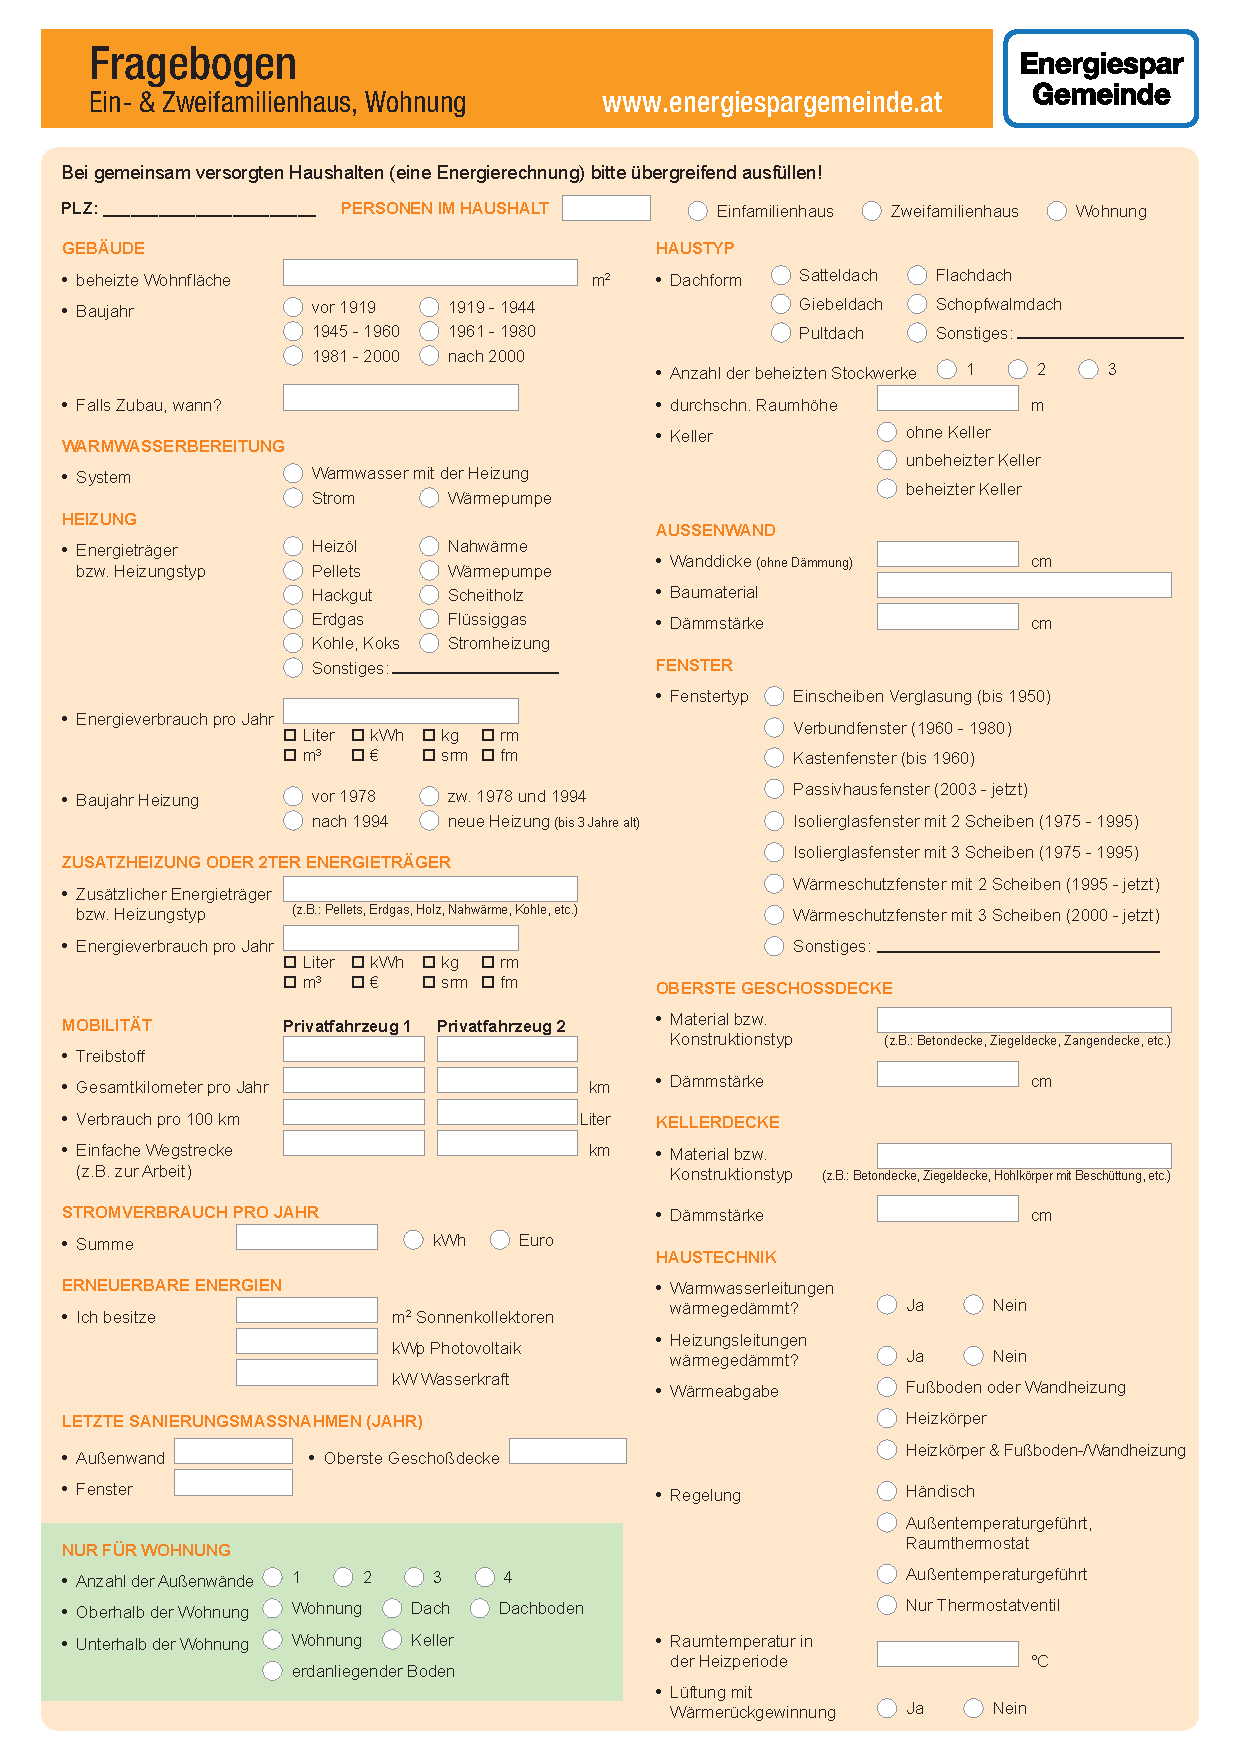
\includepdf[pages=1-,width=\textwidth,frame=true,pagecommand={}]{images/fragebogen}
\end{LaTeXCode}
%
Die eingebundenen Seiten werden durch \verb!width=\textwidth! automatisch auf
die Textbreite des \latex-Dokuments skaliert und durch \verb!frame=true! mit
einer Umrandung versehen.

Dieses Beispiel geht davon aus, dass das externe PDF-Dokument im
A4-Seitenformat ist. Bei anderen Formaten muss man die Skalierung
möglicherweise "händisch" einstellen, falls die Seiten zu hoch werden (\zB\
mit \verb!width=0.9\textwidth!).

Wichtig ist auch, dass bei dem externen PDF-Dokument alle verwendeten
\emph{Schriften} (Fonts) korrekt und vollständig \emph{eingebettet} sind, da
ansonsten das von \latex erzeugte PDF-Dokument nicht unabhängig von der
Systemumgebung ist!


\section{Verweise auf eingebundene PDF-Seiten}

Möchte man im Text auf bestimmte PDF-Seiten verweisen, so ist es am
Einfachsten, die Seiten einzeln zu importieren und jeweils mit einem
\emph{Label} zu versehen, wie in diesem Beispiel:
%
\begin{LaTeXCode}[numbers=none]
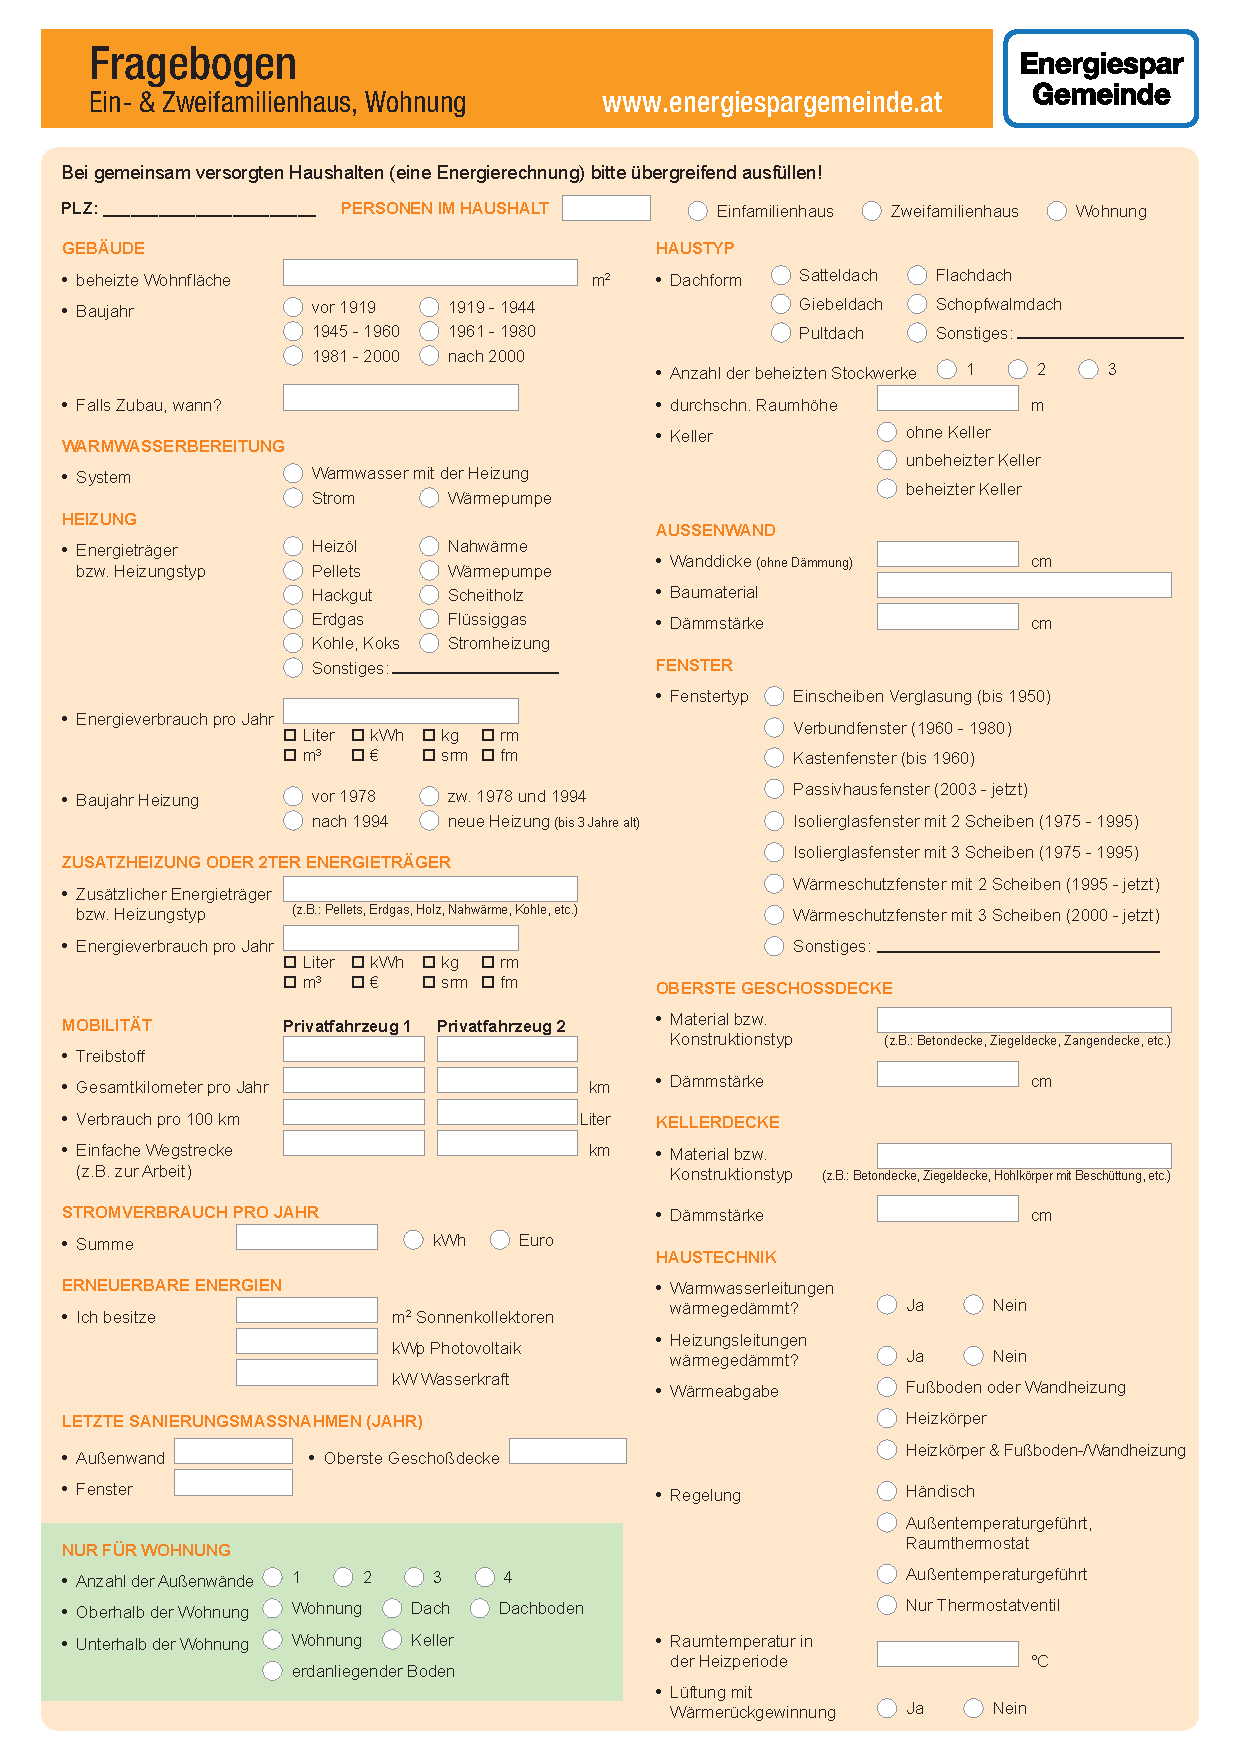
\includepdf[pages=1,width=\textwidth,frame=true,
		pagecommand={\label{PDF1}}]{images/fragebogen}
\includepdf[pages=2,width=\textwidth,frame=true,
		pagecommand={\label{PDF2}}]{images/fragebogen}
\end{LaTeXCode}
%
In diesem Fall könnte man beispielsweise mit \verb!\pageref{PDF2}! die
aktuelle Seitennummer der 2.\ Seite des eingebundenen PDF-Dokuments angeben.

Viele weitere Möglichkeiten (\zB\ die Angabe von Seitenintervallen) findet man
in der ausführlichen Dokumentation zum \texttt{pdfpages}-Paket.

% Und hiermit werden die PDF-Seiten tatsächlich eingebunden:
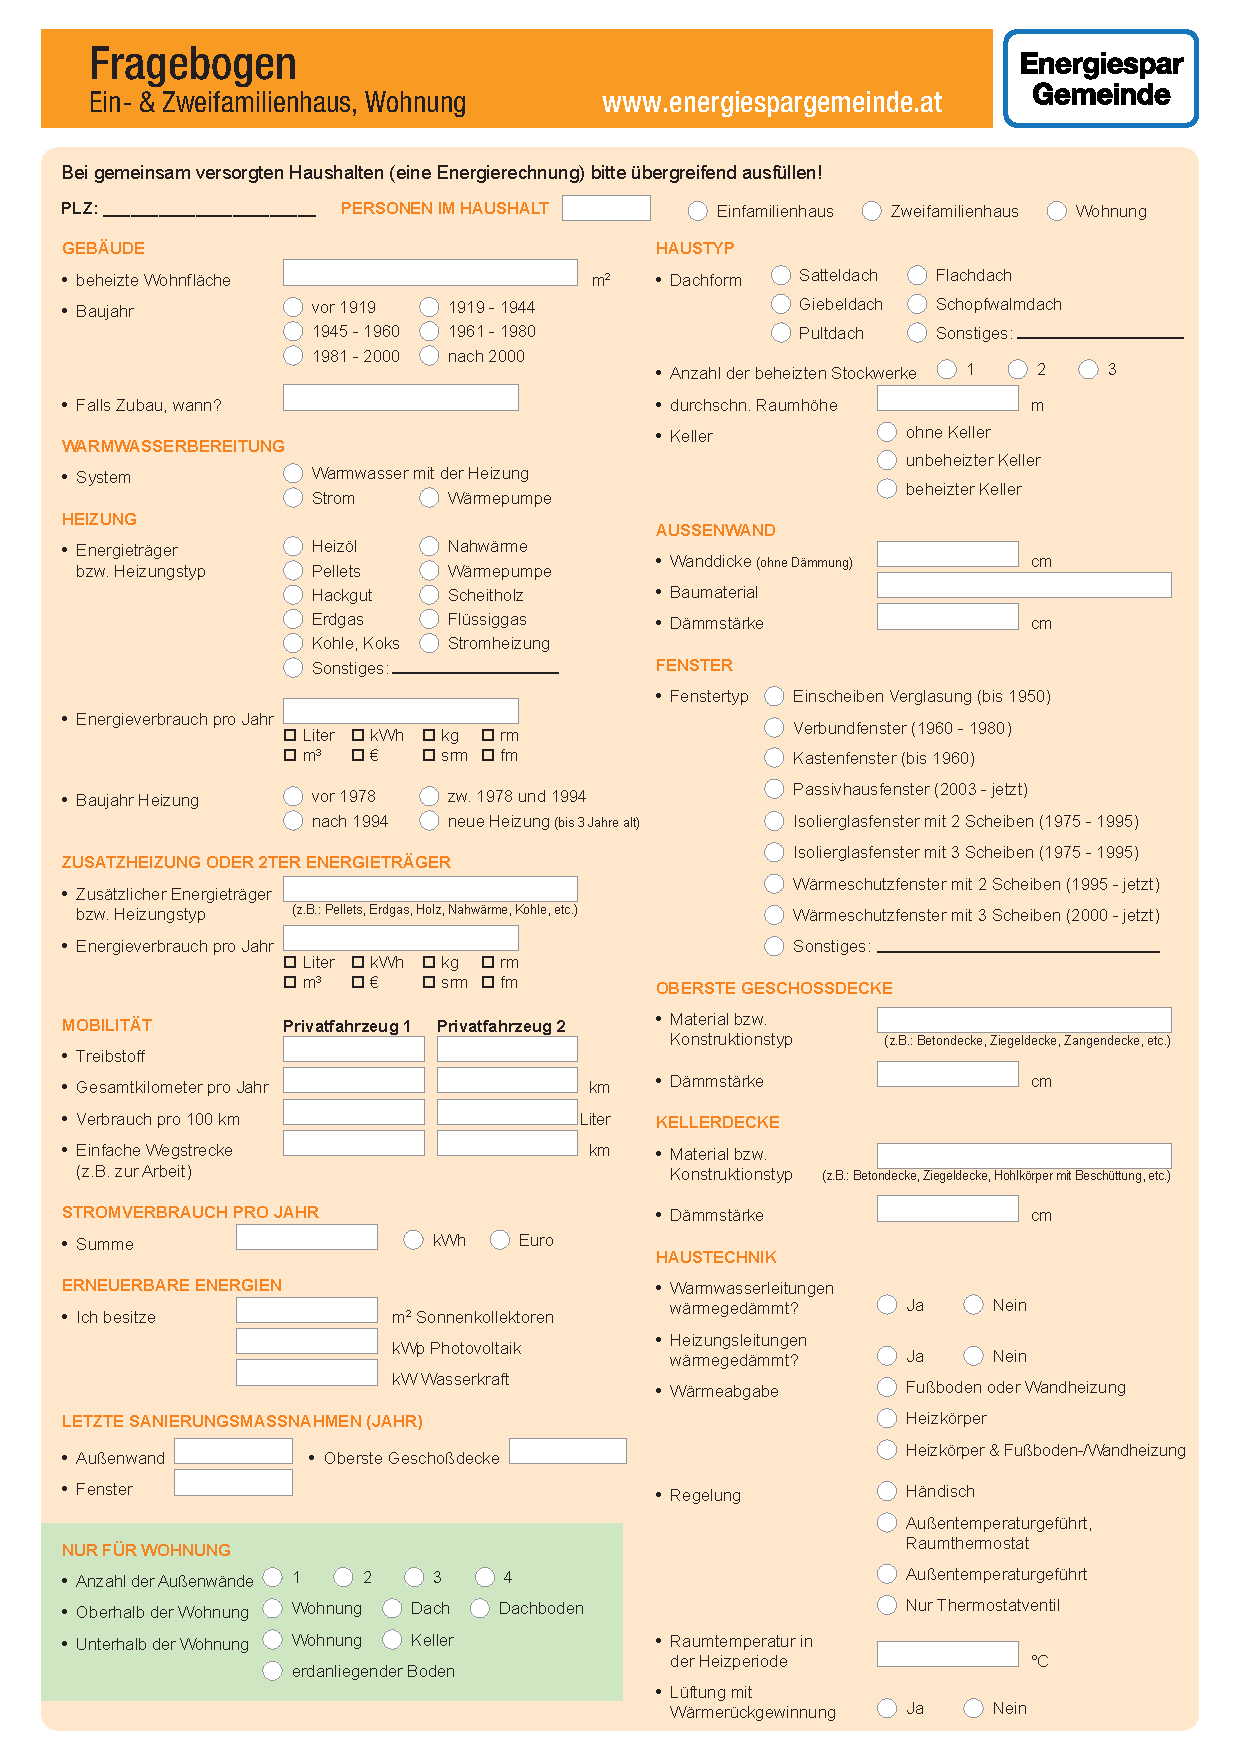
\includepdf[pages=1-,width=\textwidth,frame=true,pagecommand={}]{images/fragebogen}



 % Chronologische Liste der Änderungen
\chapter{\latex-Quellcode}
\label{app:latex}

\section*{Hauptdatei \texttt{main.tex}}

\paragraph{Anmerkung:}
Das sollte nur ein \emph{Beispiel} für die Einbindung von Quellcode
in einem Anhang sein. Die dazu verwendeten Anweisungen sind folgende:
%
\begin{LaTeXCode}[numbers=none]
\begin{footnotesize}
	\verbatiminput{main.tex}
\end{footnotesize}
\end{LaTeXCode}
%
Natürlich ist der \latex-Quellcode der eigenen Abschlussarbeit meist
\emph{nicht} interessant genug, um ihn hier wiederzugeben!

\begin{footnotesize}
	\verbatiminput{main.tex}
\end{footnotesize}





 % Quelltext dieses Dokuments

%%%-----------------------------------------------------------------------------
\backmatter                          % Schlussteil (Quellenverzeichnis und dgl.)
%%%-----------------------------------------------------------------------------

\MakeBibliography % Quellenverzeichnis

%%%-----------------------------------------------------------------------------
% Messbox zur Druckkontrolle
%%%-----------------------------------------------------------------------------

\chapter*{Messbox zur Druckkontrolle}



\begin{center}
{\Large --- Druckgröße kontrollieren! ---}

\bigskip

\calibrationbox{100}{50} % Angabe der Breite/Hoehe in mm

\bigskip

{\Large --- Diese Seite nach dem Druck entfernen! ---}

\end{center}



%%%-----------------------------------------------------------------------------
\end{document}
%%%-----------------------------------------------------------------------------
